% enable this to activate the version for PRINT
% disable this to make the pdf symmetric and without white pages
% => asymmetric alternating left/right margins
% \newcommand*{\printversion}{}%

%% | ---------------- document meta information --------------- |

\newcommand{\Author}{Michal Kamler}
\newcommand{\Department}{Department of Cybernetics}
\newcommand{\Supervisor}{MSc. Manuel Boldrer, Ph.D.}
% \newcommand{\SupervisorSpecialist}{Ing. My Specialist, Ph.D.}
\newcommand{\Programme}{Electrical Engineering and Information Technology}
\newcommand{\Field}{Cybernetics and Robotics}
\newcommand{\Title}{Development of a Safe Flocking\\[0.5em] Algorithm for UAVs Using 3D\\[0.5em] Lidar and Collaborative\\[1.0em] Multi-Robot Coordination}
\newcommand{\Keywords}{TODOUnmanned Aerial Vehicles, Automatic Control}
\newcommand{\KlicovaSlova}{Bezpilotní Prostředky, Automatické Řízení}
\newcommand{\Year}{2025}
\newcommand{\Month}{May}
\newcommand{\Date}{\Month~\Year}
\newcommand{\Location}{Prague}

%% | ---------------------- configuration --------------------- |

% most of the configuration stuff happens here
%!TEX root = ../main.tex

%% | ----------------------- page setup ----------------------- |

% define documentclass based on the print/screen version of the document
\pdfoutput=1
\ifdefined\printversion
  \documentclass[a4paper,11pt,twoside,openright]{book}
\else
  \documentclass[a4paper,11pt,twoside,openany]{book}
\fi

% define how "clearpage" works with the print/screen version of the document
\newcommand{\conditionalClearPage}{
  \ifdefined\printversion
    \cleardoublepage
  \else
    \clearpage
  \fi
}

%% | ----------------- commonly used packages ----------------- |

\usepackage[english]{babel}
\usepackage[utf8]{inputenc}
\usepackage{csquotes}
\usepackage{amsmath,amsfonts,amssymb,bm}
\usepackage{nicefrac}
\usepackage{algorithm,algpseudocode}
\usepackage[title,titletoc]{appendix}
\usepackage{latexsym}
\usepackage{a4wide}
\usepackage{color}
\usepackage{indentfirst}
\usepackage{graphicx}
\usepackage{fancyhdr,lastpage}
\usepackage{longtable}
\usepackage{pifont}
\usepackage{makeidx}
\usepackage{multirow}
\usepackage{dcolumn}
\usepackage{epstopdf}
\usepackage{url}
\usepackage{listings}
\usepackage{relsize}
\usepackage{pdfpages}
\usepackage{url}
\usepackage{lipsum}
\usepackage{isotope}
\usepackage{verbatim}
\usepackage{xcolor}
\usepackage{tcolorbox}
\usepackage[colorlinks]{hyperref}
\usepackage{multicol}
\usepackage{subfig}
\usepackage[export]{adjustbox}

\usepackage{svg}

% print version has different margins to accommodate the spine of the book
% do not move this around, or it stops working
\ifdefined\printversion
  \usepackage[a4paper,margin=3.2cm,inner=3.4cm,outer=2.0cm]{geometry}
\else
  \usepackage[a4paper,margin=3.2cm,inner=2.7cm,outer=2.7cm]{geometry}
\fi

\hyphenation{}

%% | --------------------- custom commands -------------------- |

\definecolor{cvutblue}{cmyk}{1, 0.43, 0, 0}

% set itemize: bullets type and color
\renewcommand{\labelitemi}{\textcolor{cvutblue}{\raisebox{.45ex}{\rule{.8ex}{.8ex}}}}
\renewcommand{\labelitemii}{\textcolor{cvutblue}{\raisebox{.45ex}{\rule{.8ex}{.8ex}}}}
\renewcommand{\labelitemiii}{\textcolor{cvutblue}{\raisebox{.45ex}{\rule{.8ex}{.8ex}}}}
\renewcommand{\labelitemiv}{\textcolor{cvutblue}{\raisebox{.45ex}{\rule{.8ex}{.8ex}}}}


%% | ---------------------- abbreviations --------------------- |

\usepackage[printonlyused]{acronym}

% use to change margins around abbreviations block
\def\changemargin#1#2{\list{}{\rightmargin#2\leftmargin#1}\item[]}
\let\endchangemargin=\endlist

%% | -------------------- hyper links setup ------------------- |
\hypersetup{
  linkcolor=black,
  anchorcolor=black,
  citecolor=cvutblue,
  filecolor=black,
  menucolor=black,
  runcolor=black,
  urlcolor=cvutblue
}


%% | -------------------------- tikz -------------------------- |

\usepackage{tikz}
\usepackage{pgfplots}
\pgfplotsset{compat=1.14}
\usetikzlibrary{backgrounds,arrows,automata,shapes,positioning,calc,through,spy,shapes,shapes.geometric,shapes.multipart,fit,patterns,fadings}
\pgfdeclarelayer{background}
\pgfdeclarelayer{foreground}
\pgfsetlayers{background,main,foreground}

%% | ------------ siunitx for units of measurements ----------- |

\usepackage{siunitx}
\DeclareSIUnit \parsec {pc}
\DeclareSIUnit \electronvolt {eV}
\DeclareSIUnit \pixel {px}
\DeclareSIUnit \arcmin {arcmin}
\DeclareSIUnit \erg {erg}
\DeclareSIUnit \joul {J}

%% | --------------- change formatting of lists --------------- |

\usepackage{enumitem}
\setlist{nosep}

\renewcommand{\labelenumi}{(\roman{enumi})}

%% | -------------------- table of contents ------------------- |

\usepackage[subfigure]{tocloft}

\tocloftpagestyle{plain}

%% | ----------------- formatting of a chapter ---------------- |

\usepackage{titlesec}

\titleformat{\chapter}[hang]{}{\color{cvutblue}\rule[-0.03cm]{0.50cm}{0.50cm}}{3.2\parskip}{\normalfont\bfseries\LARGE\thechapter\hspace{0.5cm}}
\titlespacing*{\chapter}{0pt}{-1em}{1.5em}

%% | ----------------- formatting of a section ---------------- |

\titleformat{\section}[hang]{}{\hspace{0.11cm}\color{cvutblue}\rule[-0.02cm]{0.30cm}{0.30cm}}{3.7\parskip}{\normalfont\bfseries\large\thesection\hspace{0.5cm}}
\titlespacing*{\section}{0pt}{1em}{0.5em}

\titleformat{name=\section,numberless}[block]
{\normalfont\large\bfseries}{}{0pt}{\large}
% {?}{before}{after}
\titlespacing*{name=\section,numberless}{0pt}{-1em}{2em}

%% | --------------- formatting of a subsection --------------- |

\titleformat{\subsection}[hang]{}{\hspace{0.16cm}\color{cvutblue}\rule[0.03cm]{0.20cm}{0.20cm}}{4.0\parskip}{\normalfont\bfseries\normalsize}
\titlespacing*{\subsection}{0pt}{1em}{0.5em}



%% | ------------------------ biblatex ------------------------ |

% \usepackage[backend=bibtex,defernumbers=true,style=ieee,sorting=ydnt,sortcites=true]{biblatex}
\usepackage[backend=bibtex,defernumbers=true,style=ieee,sorting=none,sortcites=true]{biblatex}

% define the source file with bibliography
\addbibresource{main.bib}

\renewcommand*{\bibfont}{\Font}

% add suffix "a" to publications containing the keyword "mine"
% add suffix "c" to publications containing the keyword "mine" && "core"
\DeclareFieldFormat{labelnumber}{%
  \ifkeyword{mine}
    {\ifkeyword{core}
      {{\number\numexpr#1}c}%
      {{\number\numexpr#1}a}%
    }%
    {#1}%
}

\DeclareCiteCommand{\tabcite}%[\mkbibbrackets]
  {\usebibmacro{cite:init}%
   \usebibmacro{prenote}}
  {\usebibmacro{citeindex}%
   \usebibmacro{cite:comp}}
  {}
  {\usebibmacro{cite:dump}%
   \usebibmacro{postnote}}

% define fullciteinbox command
\definecolor{light-gray}{gray}{0.95}
\newcommand{\fullciteinbox}[2]{%

\DeclareCiteCommand{\fullcite}
{\usebibmacro{prenote}}
{\clearfield{addendum}%
  \usedriver
  {\defcounter{minnames}{6}%
  \defcounter{maxnames}{6}}
{\thefield{entrytype}}}
{\multicitedelim}
{\usebibmacro{postnote}}

\begin{tcolorbox}[opacityfill=0.05,width=\textwidth,colback={cvutblue},colframe={cvutblue},title={}]%
\ifx&#2&
\else
  \textbf{#2}:\\\\
\fi
\begin{minipage}[t]{0.07\linewidth}%
\raggedright%
\cite{#1}%
\end{minipage}%
\begin{minipage}[t]{0.93\linewidth}%
\fullcite{#1}%
\end{minipage}%
\end{tcolorbox}%
%}%
\vspace{-0.3em}
}%

% change the bibliography font style
% does not compile without this
\let\bibfont\small

% this is used to print citations of author's work
\defbibenvironment{mycitations}
{\itemize}
{\enditemize}
{\item}

%% | ---------------------- custom macros --------------------- |

\newcommand{\strong}[1]{\textbf{#1}}
\newcommand{\coord}[1]{\textbf{#1}}
\newcommand{\norm}[1]{\left\lvert#1\right\rvert}
\newcommand{\m}[1]{\ensuremath{\mathbf{#1}}}
\newcommand\numberthis{\addtocounter{equation}{1}\tag{\theequation}}
\newcommand{\add}[1]{{\color{green} {#1}}}
\newcommand{\todo}[1]{{\color{red} TODO {#1}}}
\newcommand{\updated}[1]{{\color{blue} {#1}}}
\newcommand{\real}{\mathbb{R}}
\newcommand{\red}[1]{{\color{red} #1}}
\newcommand{\minus}{\scalebox{0.75}[1.0]{$-$}}
\newcommand{\plus}{\scalebox{0.8}[0.8]{$+$}}
\newcommand{\figvspace}{\vspace{-1em}}

% referencing
\newcommand{\reffig}[1]{Fig.~\ref{#1}}
\newcommand{\reflst}[1]{Lst.~\ref{#1}}
\newcommand{\refalg}[1]{Alg.~\ref{#1}}
\newcommand{\refsec}[1]{Sec.~\ref{#1}}
\newcommand{\reftab}[1]{Table~\ref{#1}}
\newcommand{\refeq}[1]{\eqref{#1}}

%% | ----------------- listings - showing code ---------------- |

\usepackage{listings}     
\usepackage{lstautogobble}  % Fix relative indenting
\usepackage{color}          % Code coloring
\usepackage{zi4}            % Nice font

\definecolor{bluekeywords}{rgb}{0.13, 0.13, 1}
\definecolor{greencomments}{rgb}{0, 0.5, 0}
\definecolor{redstrings}{rgb}{0.9, 0, 0}
\definecolor{graynumbers}{rgb}{0.5, 0.5, 0.5}

\usepackage{listings}
\lstset{
    autogobble,
    columns=fullflexible,
    showspaces=false,
    showtabs=false,
    breaklines=true,
    showstringspaces=false,
    breakatwhitespace=true,
    escapeinside={(*@}{@*)},
    commentstyle=\color{greencomments},
    keywordstyle=\color{bluekeywords},
    stringstyle=\color{redstrings},
    numberstyle=\color{graynumbers},
    basicstyle=\ttfamily\footnotesize,
    frame=l,
    framesep=12pt,
    xleftmargin=12pt,
    tabsize=4,
    captionpos=b
}

%% | -------------------- layout parameters ------------------- |

% no indent, free space between paragraphs
\setlength{\parindent}{1cm}
\setlength{\parskip}{1ex plus 0.5ex minus 0.2ex}

% offsets the head down
\setlength{\headheight}{18pt}

% foot line
\renewcommand{\footrulewidth}{0.4pt}

%% | -------------- define the 'full' page style -------------- |

\fancypagestyle{full}{%
  % \fancyhf{} % This is a more concise way to clear everything
  % \renewcommand{\headrulewidth}{0.4pt} % Or your preferred value for the header rule
  % \renewcommand{\footrulewidth}{0pt}   % No rule for the footer, or set as desired

  \fancyhead[LO]{\leftmark}
  \fancyhead[RE]{\rightmark}


  \fancyfoot[LO]{\thepage/\pageref{LastPage}} % Page number on the Left
  \fancyfoot[RO]{CTU in Prague}             % "CTU in Prague" on the Right

  \fancyfoot[LE]{CTU in Prague}             % "CTU in Prague" on the Left
  \fancyfoot[RE]{\thepage/\pageref{LastPage}} % Page number on the Right

  % \fancyfoot[C]{} % You can add this for explicitness if you wish
}




% \fancypagestyle{full}{%

%   % clear the default layout
%   \fancyhead{}
%   \fancyfoot{}

%   % page header
%   \fancyhead[LO]{\leftmark}
%   \fancyhead[RE]{\rightmark}
%   \fancyhead[LE,RO]{\thepage/\pageref{LastPage}}

%   % page footer
%   \fancyfoot[L]{CTU in Prague}
%   \fancyfoot[R]{\Department}
%   \fancyfoot[C]{}
% }

%% | -------------- define the 'plain' page style ------------- |

\fancypagestyle{plain}{%

  % clear the default layout
  \fancyhead{}
  \fancyfoot{}

  % page header
  % \fancyhead[LE,RO]{\thepage}
}

%% | -------------- Adjust style of chapter names ------------- |

\renewcommand{\chaptermark}[1]{\markboth{\MakeUppercase{\thechapter.\ #1}}{}}

%% | -------- European layout, no extra space after '.' ------- |

\frenchspacing

%% | ----------- adjust the style of the first page ----------- |

\makeatletter
\renewcommand\chapter{\if@openright\cleardoublepage\else\clearpage\fi
                    \thispagestyle{full}% original style: plain
                    \global\@topnum\z@
                    \@afterindentfalse
                    \secdef\@chapter\@schapter}
\makeatother


%% | ---------------------- the contents ---------------------- |

\begin{document}

% this will prevent unwanted line overflows
% http://latexref.xyz/_005cfussy-_0026-_005csloppy.html
\sloppy

\pagenumbering{roman}

%% --------------------------------------------------------------
%% |                         Title page                         |
%% --------------------------------------------------------------

%!TEX root = ../main.tex

\begin{titlepage}
  \begin{center}

    \textsc{\Large Czech Technical University in Prague}\\[1em]
    \textsc{\large Faculty of Electrical Engineering\\
    \Department\\
    Multi-robot Systems\\[3em]
    }
    
\includegraphics[height=4.1cm]{fig/ctu_lion.pdf}\\[3em]

    \textbf{\textsc{\Huge \Title}}\\[2em]

    \textbf{\Large Bachelor's Thesis}\\[6em]

    \textbf{\huge \Author}\\[6em]

    {\large \Location, \Date}\\[3em]

    Study programme: \Programme\\
    Branch of study: \Field\\[4em]

    \textbf{Supervisor: \Supervisor}\\

    \vspace{2pt}

  \end{center}
\end{titlepage}


% set up the page style for the "intro" pages
\pagestyle{plain}

%% --------------------------------------------------------------
%% |                       Acknowledgments                      |
%% --------------------------------------------------------------

\conditionalClearPage

%!TEX root = ../main.tex

\section*{Acknowledgments}

I would like to express my sincere gratitude to my supervisor, MSc. Manuel Boldrer, Ph.D., for his valuable guidance, helpful feedback, and for providing direction throughout the development of this thesis. 
His expertise was irreplaceable in shaping this work.

My appreciation also extends to the members of the Multi-robot Systems (MRS) group. 
I am particularly grateful for their support and practical assistance during the experimental phase, especially concerning safety during experiments and for helping me understand various technical aspects. 
Their willingness to share knowledge was very beneficial.

Finally, I would like to extend my thanks to my family for their support, patience, and encouragement throughout my studies and the writing of this thesis. 
Their belief in me has been a constant source of motivation.

\vspace{2.5cm}


%% --------------------------------------------------------------
%% |                         Assignment                         |
%% --------------------------------------------------------------

\conditionalClearPage

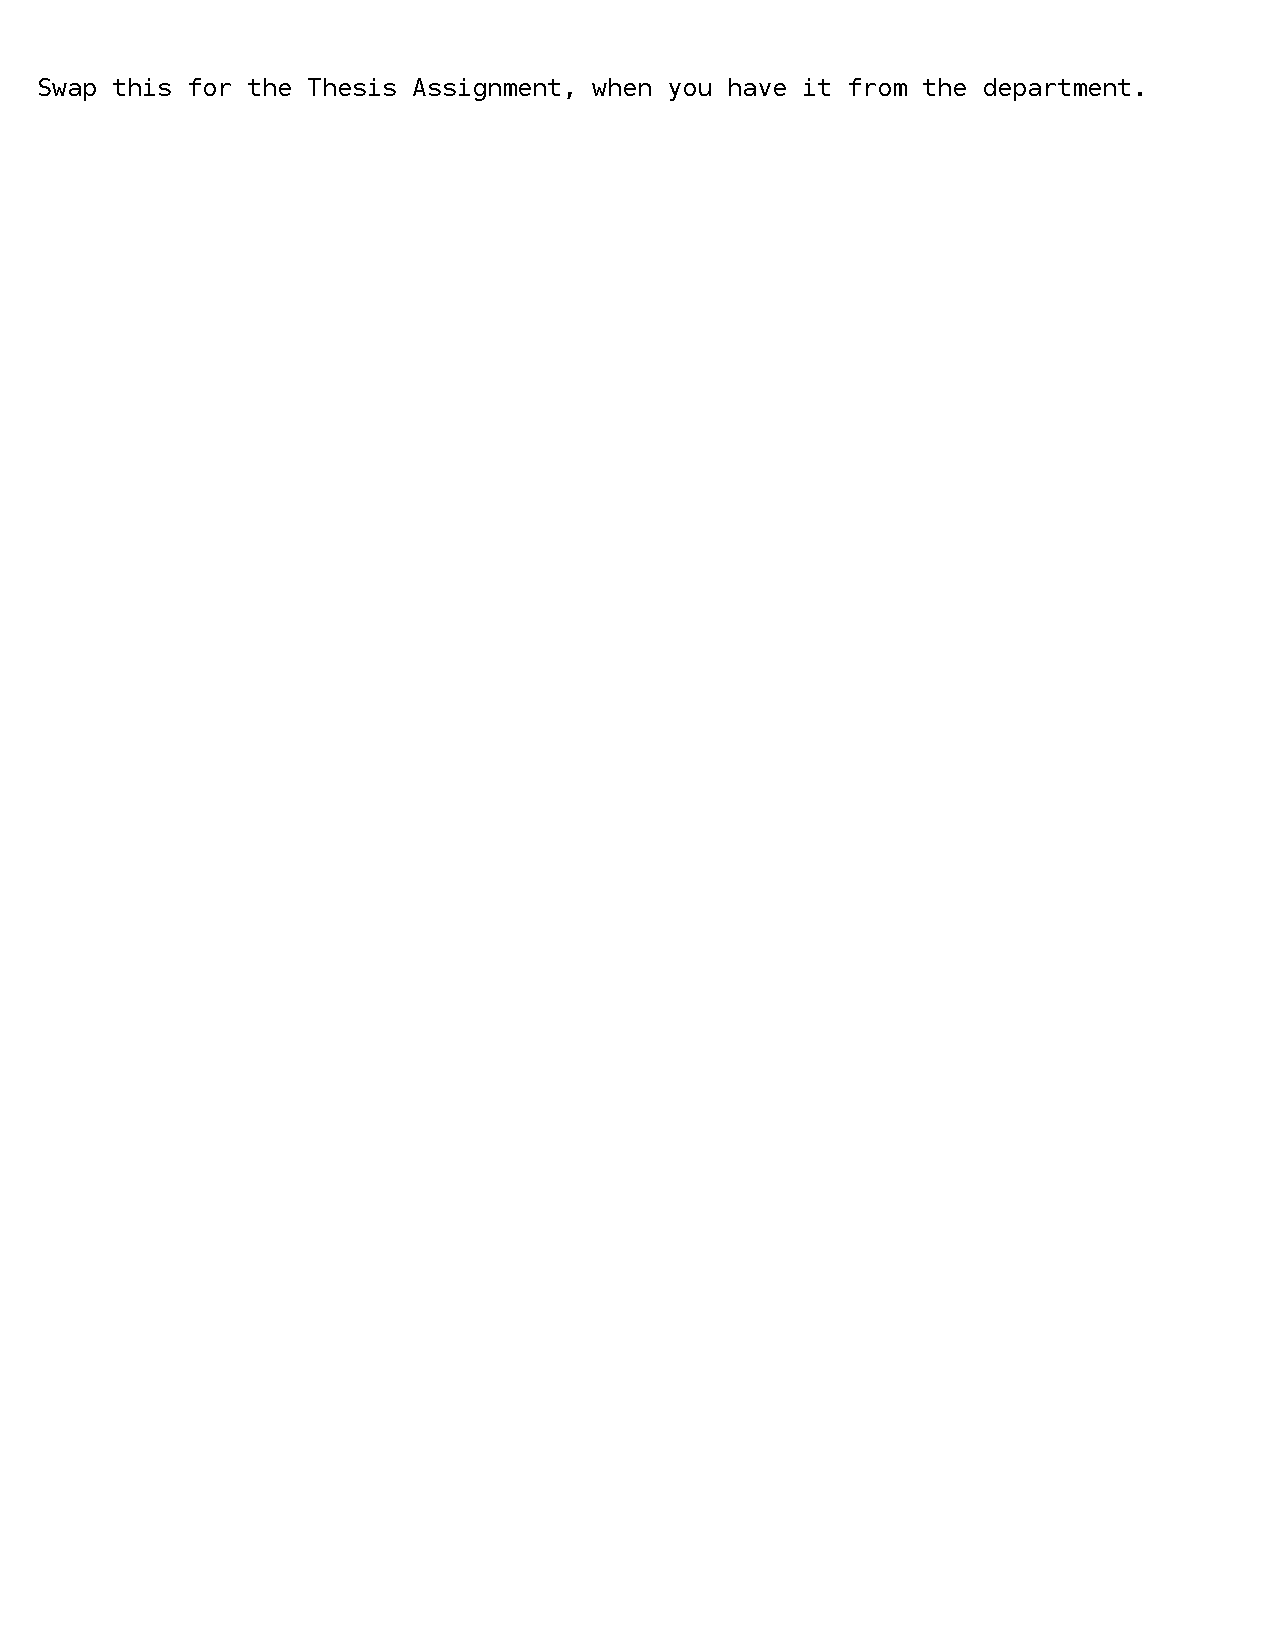
\includepdf[pages=1-2]{src/assignment.pdf}

%% --------------------------------------------------------------
%% |                         Declaration                        |
%% --------------------------------------------------------------

\conditionalClearPage

% ~\vfill{}

\section*{Declaration}
%\section*{Prohlášení autora práce}

I declare that presented work was developed independently, and that I have listed all sources of information used within, in accordance with the Methodical instructions for ob-serving ethical principles in preparation of university theses.
% Prohlašuji, že jsem předloženou práci vypracoval samostatně a že jsem uvedl veškeré použité informační zdroje v souladu s Metodickým pokynem o dodržování etických principů při přípravě vysokoškolských závěrečných prací.

\vspace{1.5cm}
~\\

Date .............................\hfill{}...............................................
% Dne.............................\hfill{}...............................................

\hfill{}~~~~~~~~~~~~~~~

\newpage{}


\includepdf[pages=1]{src/prohlaseni.pdf}

%% --------------------------------------------------------------
%% |                          Abstracts                         |
%% --------------------------------------------------------------

\conditionalClearPage

%!TEX root = ../main.tex

\begin{changemargin}{0.8cm}{0.8cm}

~\vfill{}

\section*{Abstract}
\vskip 0.5em

% Achieving effective multi-agent \ac{UAV} coordination without explicit communication, alongside robust single-agent navigation in complex, \ac{GNSS}-denied environments, presents significant research challenges.
% Therefore, developing robust algorithms capable of handling these demanding conditions is necessary.
% This thesis addresses these challenges through two primary objectives. 
% The first objective is to extend the \ac{RBL} algorithm for multi-agent coordination from two to three dimensions, introducing new rules for enhanced performance. 
% The second objective involves implementing and validating this 3D \ac{RBL} framework for single \ac{UAV} navigation in a real-world forest environment using \ac{LiDAR} sensing.

% The 2D \ac{RBL} algorithm was extended to 3D by building upon its foundational concepts and introducing new rules for vertical control. 
% For single-agent forest navigation, this 3D \ac{RBL} was integrated with \ac{LiDAR}-based perception, utilizing Point-LIO for state estimation and a voxel-based mapping approach. 
% The system was evaluated through multi-agent simulations and real-world flight experiments in a forest.

% Simulations demonstrated the successful extension of \ac{RBL} to 3D, showing improved multi-agent coordination efficiency, particularly with more agents. 
% Real-world experiments validated the effectiveness of the implemented system for autonomous point-to-point navigation in a forest, though challenges with mapping dynamic environmental elements like leaves were identified as a limitation.

% In summary, this thesis validates the modification and real-world use of the \ac{RBL} algorithm for 3D \ac{UAV} point-to-point navigation.
% While the need for enhanced mapping is needed, the results of this study significantly contribute to the development of more independent and adaptable \ac{UAV} systems.

% The study of autonomous \acp{UAV} has become a prominent sub-field of mobile robotics.


\ac{UAVs} are increasingly transitioning from open-sky operations to complex, \ac{GNSS}-denied environments, presenting significant challenges for multi-agent coordination and single-agent autonomous navigation. 
This thesis addresses these issues by first extending the \ac{RBL} algorithm from two to three dimensions for multi-\ac{UAV} communication-free coordination.
New rules were developed to manage vertical movement and enhance 3D coordination efficiency. 
Secondly, the thesis investigates the practical application of this 3D \ac{RBL} for single \ac{UAV} navigation in a challenging forest environment, utilizing onboard \ac{LiDAR} sensing.

The methodology involved adapting the core \ac{RBL} for 3D space and integrating it with real-time perception systems. 
For the single-agent navigation task, this included \ac{LiDAR}-based point cloud processing, state estimation using Point-LIO, and voxel-based environmental mapping with Bonxai. 
Strategies to minimize limitations from anisotropic sensors, such as restricted \ac{LiDAR} \ac{FOV}, were also developed. 
The proposed algorithm was evaluated through extensive simulations in the multi-agent scenario and validated with real-world experiments in a forest environment for the single-agent case.
% The extended 3D \ac{RBL} was evaluated in simulated multi-agent coordination scenarios, while the integrated single-agent system was validated through real-world flight experiments in a forest.

Simulations confirmed the successful 3D extension of the \ac{RBL} algorithm, demonstrating effective multi-agent coordination. 
Real-world experiments validated the capability of the 3D \ac{RBL}-based system for autonomous point-to-point navigation in a forest. %, as illustrated in accompanying videos \cite{aggressive_flight}, \cite{conservative_flight}. 
However, limitations were identified, particularly in the mapping system's handling of dynamic environmental elements, which occasionally led to navigation failures.% \cite{flight_fail}.

% In conclusion, this thesis demonstrates the successful adaptation and practical application of the \ac{RBL} algorithm for 3D \ac{UAV} operations. 
% It contributes a 3D extension for multi-agent coordination and a validated system for single-agent navigation in complex, real-world settings, addressing challenges posed by sensor limitations. 
% While further work on robust mapping in dynamic environments is indicated, the findings provide a valuable foundation for advancing autonomous UAV systems.




\vskip 1em

{\bf Keywords} \Keywords

\vskip 2.5cm

\end{changemargin}


%% --------------------------------------------------------------
%% |                        Abbreviations                       |
%% --------------------------------------------------------------

\conditionalClearPage

\begin{changemargin}{0.8cm}{0.8cm}

~\vfill{}

\section*{Abbreviations}

% this will print only the used abbreviations
%!TEX root = ../main.tex

\begin{acronym}
  \acro{API}[API]{Application Programming Interface}
  \acro{CTU}[CTU]{Czech Technical University}
  \acro{DOF}[DOF]{degree-of-freedom}
  \acro{FOV}[FOV]{Field of View}
  \acro{GNSS}[GNSS]{Global Navigation Satellite System}
  \acro{GPS}[GPS]{Global Positioning System}
  \acro{IMU}[IMU]{Inertial Measurement Unit}
  \acro{LKF}[LKF]{Linear Kalman Filter}
  \acro{LTI}[LTI]{Linear time-invariant}
  \acro{LiDAR}[LiDAR]{Light Detection and Ranging}
  \acro{MAV}[MAV]{Micro Aerial Vehicle}
  \acro{MPC}[MPC]{Model Predictive Control}
  \acro{MRS}[MRS]{Multi-robot Systems Group}
  \acro{ROS}[ROS]{Robot Operating System}
  \acro{RTK}[RTK]{Real-time Kinematics}
  \acro{SLAM}[SLAM]{Simultaneous Localization And Mapping}
  \acro{UAV}[UAV]{Unmanned Aerial Vehicle}
  \acro{UGV}[UGV]{Unmanned Ground Vehicle}
  \acro{UKF}[UKF]{Unscented Kalman Filter}
  \acro{RBL}[RBL]{Rule-based Lloyd Algorithm}
  \acro{ToF}[ToF]{Time-of-Flight}
  \acro{PCL}[PCL]{Point Cloud Library}
  \acro{GNSS}[GNSS]{Global Navigation Satellite System}
  \acro{3D}[3D]{three-dimensional}
  \acro{2D}[2D]{two-dimensional}
  \acro{EMI}[EMI]{Electromagnetic Interference}\
  \acro{IMU}[IMU]{Inertial Measurement Unit}
\end{acronym}


\vskip 2.5cm

\end{changemargin}

\conditionalClearPage

%% --------------------------------------------------------------
%% |                      Table of contents                     |
%% --------------------------------------------------------------

\setcounter{tocdepth}{1}
\tableofcontents

\conditionalClearPage

% set up the full page style with normal page numbering
\pagestyle{full}
\pagenumbering{arabic}

%% --------------------------------------------------------------
%% |                        introduction                        |
%% --------------------------------------------------------------
\acresetall
%!TEX root = ../main.tex

\chapter{Introduction\label{chap:introduction}}
The field of robotics has witnessed transformative advancements in recent decades, with \ac{UAVs} emerging as particularly versatile platforms. 
Their applications are rapidly expanding beyond traditional open-sky operations (agricultural surveying \cite{agricultural_survey}, powerline inspection \cite{powerline_inspection}, photogrammetry \cite{photogrammetry}) into increasingly complex scenarios, underscoring a significant trend towards autonomy. 
This growing relevance is highlighted by initiatives ranging from commercial use cases, such as Amazon's exploration of \ac{UAV}s for package delivery and return services \cite{InsiderIntelligence_DroneDelivery}, to pioneering scientific missions like 
  the Ingenuity helicopter's collaboration with the Perseverance rover on Mars \cite{NASA_Ingenuity}, which demonstrated the potential of aerial robotic support in extraterrestrial exploration.

However, the widespread and effective deployment of \ac{UAV}s, particularly in coordinated multi-agent systems and challenging environments, presents substantial research challenges. 
One critical area is multi-robot coordination, which requires robust methods for agents to perceive and react to each other efficiently. 
While distributed swarms can achieve scalability even with explicit communication, for instance, through the implementation of ad-hoc networks, developing strategies that minimize dependence on such communication is important. 
This is because communication channels are often prone to unreliability, including delays, failures, and packet losses, which can decrease performance.
Simultaneously, autonomous navigation in complex, unstructured environments, often characterized by the absence or unreliability of \ac{GNSS} signals, remains a significant barrier.

Addressing these navigational challenges often involves advanced perception systems. 
\ac{LiDAR} technology offers distinct advantages in providing accurate and fast spatial data compared to alternatives like depth cameras or computationally expensive neural network-based depth estimation from monocular images. 
While the precise real-time state estimation of the \ac{UAV} within such \ac{GNSS}-denied environments is a complex problem in itself (often addressed by dedicated \ac{SLAM} algorithms, which are utilized as existing tools in this work rather than being a primary research focus), the ability to perceive and navigate through these cluttered spaces is the main objective. 
% This thesis explores several challenges by first investigating approaches for \ac{UAV} coordination in defined multi-agent scenarios, and subsequently focusing on single \ac{UAV} navigation in complex environments leveraging perceived information from onboard sensors.
This thesis explores several challenges by first investigating approaches for \ac{UAV} coordination in simulated multi-agent scenarios with predefined configurations, such as formations involving multiple \ac{UAV}s crossing in a circular or spherical pattern. 
Subsequently, it focuses on single \ac{UAV} navigation in complex environments, such as forests, using perceived information from onboard sensors.

\section{Related Works}

  This research primarily addresses multi-agent coordination and autonomous UAV navigation in complex environments. 
  This section briefly reviews key literature to contextualize the thesis.
  \subsection{Foundational Work}
    This thesis directly extends the \ac{RBL} algorithm presented in \cite{rbl_paper}. 
    While the original work showed promise for distributed multi-agent navigation, it was limited to two-dimensional (2D) scenarios. 
    This thesis addresses the need to adapt \ac{RBL} for three-dimensional (3D) \ac{UAV} operations, which involve vertical movement and spatial complexity.

  \subsection{Multi-Agent Coordination and Navigation Approaches}
    Enabling multiple robots to navigate and coordinate effectively is a significant challenge that has led to a variety of research directions.
    A fundamental distinction lies in the system's architecture: centralized approaches rely on a global controller for optimal, system-wide decisions, often suitable for structured settings like warehouses \cite{warehouse_intro}, but face scalability and communication bottlenecks.
    In contrast, distributed or distributed methods allow individual agents to make decisions based on local information.
    This approach generally improves scalability, but do not provide an optimal solution for each agent. 
    Distributed methods can be further categorized into three main types: 
    \begin{itemize}
      \item \textbf{Reactive Methods: } \\
        These methods \cite{reactive1, reactive2} make robots react immediately to what their sensors see in their current local area. 
        % They are generally fast and simple, but because they don't look far ahead, robots using them can sometimes get stuck or into repetitive loops (deadlocks), unable to reach their goals.
        They are generally fast and simple, but because they don't look far ahead, robots using them can sometimes get stuck in deadlocks (e.g., becoming completely immobilized) or trapped in livelocks (e.g., engaging in repetitive, non-progressive loops), preventing them from reaching their goals.
      \item \textbf{Predictive Planning Methods: } \\
        These techniques \cite{predictive1, predictive2} aim to make robots smarter by using information about nearby robots or the environment to plan better routes. 
        This can lead to improved performance and help avoid getting stuck. 
        However, these methods often need more computational power and sometimes they need to heavily rely on communication between robots.
      \item \textbf{Learning-Based Methods: } \\
        These newer approaches \cite{rl1, rl2} use techniques like Reinforcement Learning to teach robots how to navigate by learning from experience or data. 
        They can be very good at handling complex situations. 
        However, it's often hard to guarantee they will always be safe or reach their goal, and they might not work well in situations very different from what they were trained on.
    \end{itemize}
    \ac{RBL} algorithm, which is a core focus of this thesis, is fundamentally a reactive approach that has been enhanced with specific rules designed to prevent common deadlock situations.


\section{Problem Statement}
  The increasing deployment of \ac{UAV}s in diverse and complex scenarios requires robust autonomous navigation and coordination capabilities. 
  While foundational algorithms like the \ac{RBL} algorithm, as presented in \cite{rbl_paper}, have shown promise for distributed multi-agent navigation, their application has primarily been explored in 2D planar environments. 
  This thesis identifies and addresses two key problem areas emerging from these limitations and the demands of real-world applications:
  \begin{enumerate}
    \item \textbf{Limitations of 2D Algorithms for 3D Multi-Agent Coordination: } \\
      The direct application of 2D coordination strategies to three-dimensional space can be incomplete. 
      Adding the vertical dimension makes the navigation problem harder, as it introduces more agent interactions and demands new rules for efficient goal convergence.
      Existing 2D algorithm lacks the methods to effectively control vertical exploration and coordination.
      \begin{itemize}
        \item \textbf{Problem 1: } \\
        Given $N$ \ac{UAV}s operating in a shared 3D environment, there is a need to develop a distributed coordination algorithm that extends planar navigation principles to efficiently steer each agent from its initial position to a goal region in three dimensions, while ensuring safety and operating without communication. 
        This involves the challenge of designing rules that effectively manage the vertical dimension without compromising the scalability and deadlock-avoidance properties of the foundational algorithm.
      \end{itemize}
    \item \textbf{Transitioning Navigation Algorithms to Complex, GNSS-Denied Real-World Environments: } \\
      Beyond theoretical coordination in open spaces, a critical challenge lies in applying navigation algorithms to single \ac{UAV}s operating in complex, unstructured, and GNSS-denied environments, such as dense forests. 
      For successful operation in these settings, \ac{UAV}s must effectively perceive their surroundings, accurately estimate their own state, and adequately represent the environment.
      \begin{itemize}
        \item \textbf{Problem 2: } \\
        Given a single \ac{UAV} equipped with sensors like \ac{LiDAR}, operating in a cluttered, GNSS-denied environment (e.g., a forest), the problem is to enable reliable autonomous point-to-point navigation. 
        This requires not only a suitable 3D navigation algorithm (such as an extension of \ac{RBL}) but also its effective integration with real-time sensor data processing for obstacle detection and accurate state estimation, all while addressing additional challenge of navigating with anisotropic onboard sensors and their inherent limitations (e.g., restricted fields of view).
      \end{itemize}
  \end{enumerate}

\section{Contributions}
  This thesis presents four key contributions to the field of autonomous \ac{UAV} navigation and multi-agent coordination.
  \begin{itemize}
    \item Extension of the \ac{RBL} algorithm to three dimensions, development of new rules to enhance multi-\ac{UAV} coordination and efficiency in 3D space.
    % \item Extension of the \ac{RBL} algorithm to three dimensions.
    % \item Development of new rules for 3D \ac{RBL} coordination and efficiency.
    % \item Practical integration for real-world \ac{UAV} navigation with respect to sensor limitations.
    \item Development and practical integration of navigation strategy that effectively address the challenges posed by anisotropic onboard sensors (e.g., limited \ac{FOV}). 
    This work advances beyond common isotropic sensing assumptions, often assumed in foundational algorithms like \ac{RBL}, to enable navigation in realistic environments.
    % \item Experimental validation in simulated and real-world forest environment.
    \item Experimental validation of the developed algorithm through simulations and real-world trials in challenging forested environments.
  \end{itemize}

\section{Mathematical Notation}

TODO

\begin{table*}[!h]
  \scriptsize
  \centering
  \noindent\rule{\textwidth}{0.5pt}
  \begin{tabular}{lll}
    % 2d, 3d, 

    $\mathcal{N}_i$ & set of neighboring agents for the i-th agent\\



    $\mathbf{x}$, $\bm{\alpha}$ & vector, pseudo-vector, or tuple\\
    $\mathbf{\hat{x}}$, $\bm{\hat{\omega}}$& unit vector or unit pseudo-vector\\
    $\mathbf{\hat{e}}_1, \mathbf{\hat{e}}_2, \mathbf{\hat{e}}_3$ & elements of the \emph{standard basis} \\
    $\mathbf{X}, \bm{\Omega}$ & matrix \\
    $\mathbf{I}$ & identity matrix \\
    $x = \mathbf{a}^\intercal\mathbf{b}$ & inner product of $\mathbf{a}$, $\mathbf{b}$ $\in \mathbb{R}^3$\\
    $\mathbf{x} = \mathbf{a}\times\mathbf{b}$ & cross product of $\mathbf{a}$, $\mathbf{b}$ $\in \mathbb{R}^3$\\
    $\mathbf{x} = \mathbf{a}\circ\mathbf{b}$ & element-wise product of $\mathbf{a}$, $\mathbf{b}$ $\in \mathbb{R}^3$ \\
    $\mathbf{x}_{(n)}$ = $\mathbf{x}^\intercal\mathbf{\hat{e}}_n$ & $\mathrm{n}^{\mathrm{th}}$ vector element (row), $\mathbf{x}, \mathbf{e} \in \mathbb{R}^3$\\
    $\mathbf{X}_{(a,b)}$ & matrix element, (row, column)\\
    $x_{d}$ & $x_d$ is \emph{desired}, a reference\\
    $\dot{x}, \ddot{x}, \dot{\ddot{x}}$, $\ddot{\ddot{x}}$ & ${1^{\mathrm{st}}}$, ${2^{\mathrm{nd}}}$, ${3^{\mathrm{rd}}}$, and ${4^{\mathrm{th}}}$ time derivative of $x$\\
    $x_{[n]}$ & $x$ at the sample $n$ \\
    $\mathbf{A}, \mathbf{B}, \mathbf{x}$ & LTI system matrix, input matrix and input vector\\
    \emph{SO(3)} & 3D special orthogonal group of rotations\\
    \emph{SE(3)} & \emph{SO(3)}~$\times~\mathbb{R}^3$, special Euclidean group\\
  \end{tabular}
  \noindent\rule{\textwidth}{0.5pt}
  \caption{Mathematical notation, nomenclature and notable symbols.}
  \label{tab:mathematical_notation}
\end{table*}


\chapter{Extension of the Rule-Based Lloyd Algorithm to 3D\label{chap:rbl}}
\section{Introduction}
    \subsection{Motivation}
        Motivation in using \ac{RBL} algorithm offers communication-less approach for guiding multiple agents from point A to point B.
        It requires an estimate of its position—whether through \ac{GPS}, \ac{RTK} or methods like \ac{SLAM}—along with onboard sensors that provide information about the surrounding environment, enabling it to avoid obstacles and move toward the goal.
        So far, the algorithm has mainly been tested in \ac{2D} scenarios with a fixed altitude, and the results have looked promising. 
        This were the main motivation factors to try and extend it to full \ac{3D} navigation, where altitude and sensor orientation also play a role.

    \subsection{Problem Statement}
        Many real-world robotic applications, particularly involving \ac{UAV}, require navigation within \ac{3D} environments containing obstacles. 
        While algorithms like the \ac{RBL} \cite{rbl_paper} have proven effective in \ac{2D} goal convergence, they are inherently limited when applied directly to \ac{3D} space. 
        The core problem arises because the existing \ac{RBL} algorithm is fundamentally designed for \ac{2D} planar navigation, making it unsuitable for applications like UAV operations that require navigating in \ac{3D} space.
        Specifically, there is a need to extend existing \ac{2D} algorithms to \ac{3D} while smartly incorporating vertical exploration to ensure safe, efficient, and effective navigation through crowded 3D environments without significantly compromising performance or requiring excessive computational resources. 
        This work addresses the challenge of adapting the \ac{RBL} algorithm for \ac{3D} space by developing and evaluating specific rules to control vertical movement, aiming to achieve robust 3D navigation capabilities.
        
    \subsection{Objectives}
        \begin{itemize}
            \item   Enhance the convergence speed of agents towards their goals by promoting exploration, with  focus on the vertical exploration.
            \item   Demonstrate the algorithm's enhanced applicability, achieved by extending goal placement to the z-axis.
        \end{itemize}

    \subsection{Chapter Overview}
        The principles of the \ac{RBL} algorithm, presented in \cite{rbl_paper}, form the basis of the work in this chapter. 
        These principles are clarified and modified to address the challenges of \ac{3D} extension.  
        The chapter details the fundamental principles of RBL in \ac{2D} and \ac{3D} spaces, describes the specific rules applied to enhance convergence, and concludes with a series of simulation scenarios designed to demonstrate the performance of the proposed solution.
        Finally, the chapter concludes in the presentation and evaluation of simulation experiments designed to assess the efficiency of the proposed \ac{3D} extension and the impact of the introduced vertical exploration rules.

\section{Basic principles of Rule-Based Lloyd Algorithm}

    \subsection{Overview}        
        The algorithm is a communication-less approach designed to navigate agents from point A to point B. 
        The algorithm's ability to determine each agent's position relative to its goal depends on the availability of positioning data. 
        This can be either global positioning data, such as from GPS, or relative positioning data obtained through techniques like SLAM in GNSS-denied environments, combined with sensor inputs that provide information about the agent's surrounding environment.
        These sensors can include LiDAR, depth cameras, or standard cameras with estimation techniques, allowing the agent to detect and avoid obstacles or other agents. 
        The algorithm enables autonomous navigation without requiring direct communication between agents, making it suitable for scalable and decentralized applications.

    \subsection{Applications and Limitations in 2D}
        Modern robotics relies on the capability to navigate from point A to point B.
        Navigation plays a crucial role in various robotic applications, such as \ac{UGV}s, which are commonly used in manufacturing and logistics. 
        \ac{UGV}s typically follow predefined \ac{2D} trajectories guided by visual \cite{vision_navigation}, magnetic \cite{magnetic_navigation}, or LiDAR-based navigation \cite{lidar_navigation}. 
        Additionally, \ac{2D} navigation is widely used in robotic vacuum cleaners, enabling them to systematically cover an area while avoiding obstacles.

        An obvious limitation for algorithms in \ac{2D} is scalability. 
        As the number of agents in a system increases, the complexity of managing their movements and coordination also grows significantly.
        Obstacle avoidance in \ac{2D} can also be less efficient compared to \ac{3D} environments, as agents have fewer options for evading obstacles. 
        In \ac{3D}, agents can change their altitude in addition to their horizontal trajectory, giving them more freedom to maneuver around obstacles.

    \subsection{Key Principles in 2D}
        It should be noted that most of the infromation presented here is adapted from the work detailed in \cite{rbl_paper}.
        RBL ensures convergence to the goal and provides sufficient conditions for achieving it. 
        The problem involves individual control of $N$ agents from their initial position $\mathbf{p}_i(0)$ toward a goal region, represented as circle.
        This goal region is denoted as $G(\mathbf{g}_i, r_g)$, where $\mathbf{g}_i$ is center and $r_g$ is radius of goal region. 
        The agent is progressing towards its designated destination, $\mathbf{d}_i$.
        Each agent knows its current position $\mathbf{p}_i$, encumbrance $\delta_i$, which determines safe space around agent.
        Additionally, each agent also knows the positions and encumbrances of its neighboring agents $\mathbf{\mathcal{N}_i}$, agent $j \in \mathbf{\mathcal{N}_i}$ if $||\mathbf{p}_i - \mathbf{p}_j|| \leq \frac{r_{s,i}}{\eta}$, where $r_{s,i}$ is sensing radius of the i-th agent and $\eta$ is a scaling parameter of cells.
        For simplicity $r_{s,i}$ is considered to be same for all agents, therefore $r_{s,i} = r_s$. 

        The core objective of the algorithm is to maximize the coverage cost function, which accounts for the distribution of agents and obstacles over the environment. 
        This function is expressed as:
        \begin{equation}
            J_{\text{cov}}(\mathbf{p}) = \sum_{i=1}^{N} \int_{\mathcal{V}_i} \lVert\mathbf{q}-\mathbf{p}_i\rVert^2 \varphi_i (\mathbf{q})d\mathbf{q}\text{,}
            \label{coverage_cost_function}
        \end{equation}
        where $\mathbf{p}_i$ is the position of agent $i$, $\mathcal{V}_i$ is the Voronoi cell of the i-th robot, $\lVert\mathbf{q}-\mathbf{p_i}\rVert^2$ is squared Euclidian distance between point in the mission space $\mathbf{q} \in \mathcal{Q}$ and agent's position $p_i$, 
        and $\varphi_i (\mathbf{q})$ is the weighting function.

        Voronoi cell is defined as: 
        \begin{equation}
            \mathcal{V}_i = \{q \in \mathcal{Q} \lvert \lVert \mathbf{q} - \mathbf{p}_i \rVert \leq \lVert q - \mathbf{p}_j \rVert, \forall j \neq i\}\text{.}
        \end{equation}
        For visual representation see \reffig{fig:voronoi_2d}. 

        However, this standard definition of Voronoi cells does not take into account the physical space occupied by the agents, their encumbrances. 
        To address this, a Modified Voronoi cell is introduced, which takes into account the encumbrances of agents.
        This modified version adjusts the boundaries of each Voronoi cell to account for the encumbrances of neighboring agents.
        Also to enhance the algorithm performance, the Voronoi cell are scaled using a scaling parameter $\eta \in [0, 1]$.
        The modified Voronoi cell definition is as follows:
        \begin{equation}
            \label{eq:voronoi_cell_account_encum}
            \tilde{V}_i = 
            \begin{cases}
            \{ \mathbf{q} \in Q \mid \| \mathbf{q} - \mathbf{p}_i \| \leq \eta \| \mathbf{q} - \mathbf{p}_j \| \}, & \text{if } \Delta_{ij} \leq \frac{\| \mathbf{p}_i - \mathbf{p}_j \|}{2} \\
            \{ \mathbf{q} \in Q \mid \| \mathbf{q} - \mathbf{p}_i \| \leq \eta \| \mathbf{q} - \tilde{\mathbf{p}}_j \| \}, & \text{otherwise}\text{.}
            \end{cases}
        \end{equation}
        $\forall j \in \mathcal{N}_i$, where $\Delta_{ij} = \delta_i + \delta_j$ and $\tilde{\mathbf{p}}_j = \mathbf{p}_j + 2(\Delta_{ij} - \frac{\| \mathbf{p}_i - \mathbf{p}_j \|}{2})\frac{ \mathbf{p}_i - \mathbf{p}_j }{\| \mathbf{p}_i - \mathbf{p}_j \|}$.
        The parameter $\eta$ controls the degree of ovelap or empty space between cells.
        Specifically, for the classical Voronoi cell definition ($\eta$ = 0.5), each agent needs to detect its neighbors within a distance of $2r_{s}$.
        In general each agent needs to know its neighbors within distance of $\frac{r_s}{\eta}$.

        Together with cell $\mathcal{S}_i$ defined as: 
        \begin{equation}
            \mathcal{S}_i = \{\mathbf{q} \in \mathcal{Q} | \| \mathbf{q} - \mathbf{p}_i \| \leq r_{s,i}\}\text{,}
        \end{equation}
        the cell $\mathcal{A}_i$ is obtained as $\mathcal{A}_i = \tilde{V}_i \cap \mathcal{S}_i$.

        Convergence to goal region $G(\mathbf{g}_i, r_g )$ depends on the choice of weighting function that assigns weights to points $\mathbf{q}$ in the mission space $\mathcal{Q}$.
        The weighting function $\varphi_i(\mathbf{q})$ is defined as follows: 
        \begin{equation}
            \varphi_i(\mathbf{q}) = \exp\left(-\frac{\|\mathbf{q} - \mathbf{d}_i\|}{\beta_i}\right)\text{,}
        \end{equation}
        where $\beta_i$ is the weighting factor for points $\mathbf{q}$, and $\mathbf{d}_i$ represents the current destination of the agent. 
        The destination is computed as follows:
        \begin{equation}
            \mathbf{d}_i = \mathbf{p}_i + R(\theta)(\mathbf{g}_i - \mathbf{p}_i)\text{,}
        \end{equation}
        where $R$ is the azimuthal rotation.
        Rules for changing weighting function and rotation of destination: 
        \begin{itemize}
            \item \textbf{Weighting rule}
                \begin{equation}
                    \label{eqn:beta_weighting}
                    \dot{\beta}_i(A_i) = 
                    \begin{cases}
                        -k & \text{if } \beta_i > \beta_{\min} \land \|\mathbf{c}_{A_i} - \mathbf{p}_i\| < d_1 \land \|\mathbf{c}_{A_i} - \mathbf{c}_{\mathcal{S}_i}\| > d_2  \\
                        0  & \text{if } \beta_i \leq \beta_{\min} \land \|\mathbf{c}_{A_i} - \mathbf{p}_i\| < d_1 \land \|\mathbf{c}_{A_i} - \mathbf{c}_{\mathcal{S}_i}\| > d_2  \\
                        -(\beta_i - \beta_i^D) & \text{otherwise}\text{,}
                    \end{cases}
                \end{equation}
                where the first case decreases $\beta_i$ over time, the second case ensures that $\beta_i$ does not decrease below its minimum threshold $\beta_{\min}$ (saturation) and the third case provides a general update rule when the previous conditions are not met.
            \item \textbf{Azimuth update rule}
                \begin{equation}
                    \label{eqn:azimuth_2d}
                    \dot{\theta}_i = 
                    \begin{cases}
                        k  & \text{if } \theta < \frac{\pi}{2} \land \|\mathbf{c}_{\mathcal{A}_i} - \mathbf{c}_{\mathcal{S}_i}\| > d_4 \land \|\mathbf{p}_i - \mathbf{c}_{\mathcal{A}_i}\| > d_3 \\
                        -k & \text{if } \theta > 0 \land \neg (\|\mathbf{c}_{\mathcal{A}_i} - \mathbf{c}_{\mathcal{S}_i}\| > d_4 \land \|\mathbf{p}_i - \mathbf{c}_{\mathcal{A}_i}\| > d_3) \\
                        0  & \text{otherwise}\text{,}
                    \end{cases}
                \end{equation}
                where the first case increases $\theta_i$ over time, the second case ensures that $\theta_i$ converges back when the distance constraints are not satisfied, and the third case keeps $\theta_i$ unchanged.
            \item \textbf{Azimuth reset rule}
                \begin{equation}
                    \label{eqn:azimuth_reset_2d}
                    \theta = 0 \quad \text{if } \theta = \frac{\pi}{2} \land \| \mathbf{p}_i - \mathbf{\overline{c}}_{\mathcal{A}_i} \|\text{,}
                \end{equation}
                where $\mathbf{\overline{c}}_{\mathcal{A}_i}$ represents the centroid computed from the cell $\mathcal{A}_i$, which is weighted using the unrotated destination, meaning $\mathbf{d}_i = \mathbf{g}_i$.
        \end{itemize}
        Weighted centroid is computed as follows:        
        \begin{equation}
            \mathbf{c}_{\mathcal{A}_i} = \frac{\int_{\mathcal{A}_i} \mathbf{q} \varphi_i(\mathbf{q}) \, d\mathbf{q}}{\int_{\mathcal{A}_i} \varphi_i(\mathbf{q}) \, d\mathbf{q}}\text{,}
        \end{equation}
        where \( \mathbf{q} \) represents the point in mission space, and \( \varphi_i(\mathbf{q}) \) is a weighting function. 
        The centroids for other relevant cells are computed using a similar approach, but over different sets.

        By applying the previously defined rules and computations, the RBL algorithm successfully guides agents movement toward the goal.
        However, these rules focus on rotating the centroid $\mathcal{A}_i$ in the azimuthal plane. 
        To enhance performance in a fully three-dimensional space, additional rules are required to account for elevation adjustments. 

\section{Extension of the RBL algorithm to 3D}
    \subsection{Motivation for 3D Extension}
        In many practical applications, agents must operate in three-dimensional spaces, considering not only horizontal movement but also vertical.
        A \ac{3D} extension is necessary to navigate complex environments that feature obstacles in all directions.
        In \ac{2D}, agents are restricted to a flat plane, which simplifies navigation but limits the ability to interact with objects and environments that exist in the third dimension.
        The ability to utilize vertical space can enhance energy efficiency, as agents can optimize their paths by ascending or descending to avoid obstacles or to find more favorable environmental conditions, such as discovering more open space.
        The transition from \ac{2D} to \ac{3D} also opens up possibilities for more advanced movement strategies, such as navigating through multi-level environments or optimizing trajectories by utilizing vertical space.  
        Moreover, the use of \ac{3D} models allows for more accurate representations of real-world scenarios, where elevation plays a crucial role in decision-making and task execution.


    \subsection{Differences between 2D and 3D}
        The primary distinction in the \ac{3D} extension is that each goal region is now represented as a sphere rather than a circle.  
        Similarly, the sensing cell $\mathcal{S}_i$ is also modeled as a sphere instead of a circle, allowing for a more accurate representation of the \ac{UAV}'s perception in three-dimensional space.  
        This change introduces a key modification when defining $\tilde{V}_i$: in the \ac{2D} case, a line was sufficient to slice the sensing region, whereas in \ac{3D}, a plane must be computed to properly segment the spherical sensing cell. 
        
        \begin{figure}[H]
            \centering
            \subfloat[Euclidean Voronoi Diagram in \ac{2D}] {
            
\includegraphics[width=0.48\textwidth, height=0.48\textwidth]{./fig/diagrams/Euclidean_Voronoi_diagram.jpg}
            \label{fig:voronoi_2d}
            }
            \subfloat[Euclidean Voronoi Diagram in \ac{3D}] {
            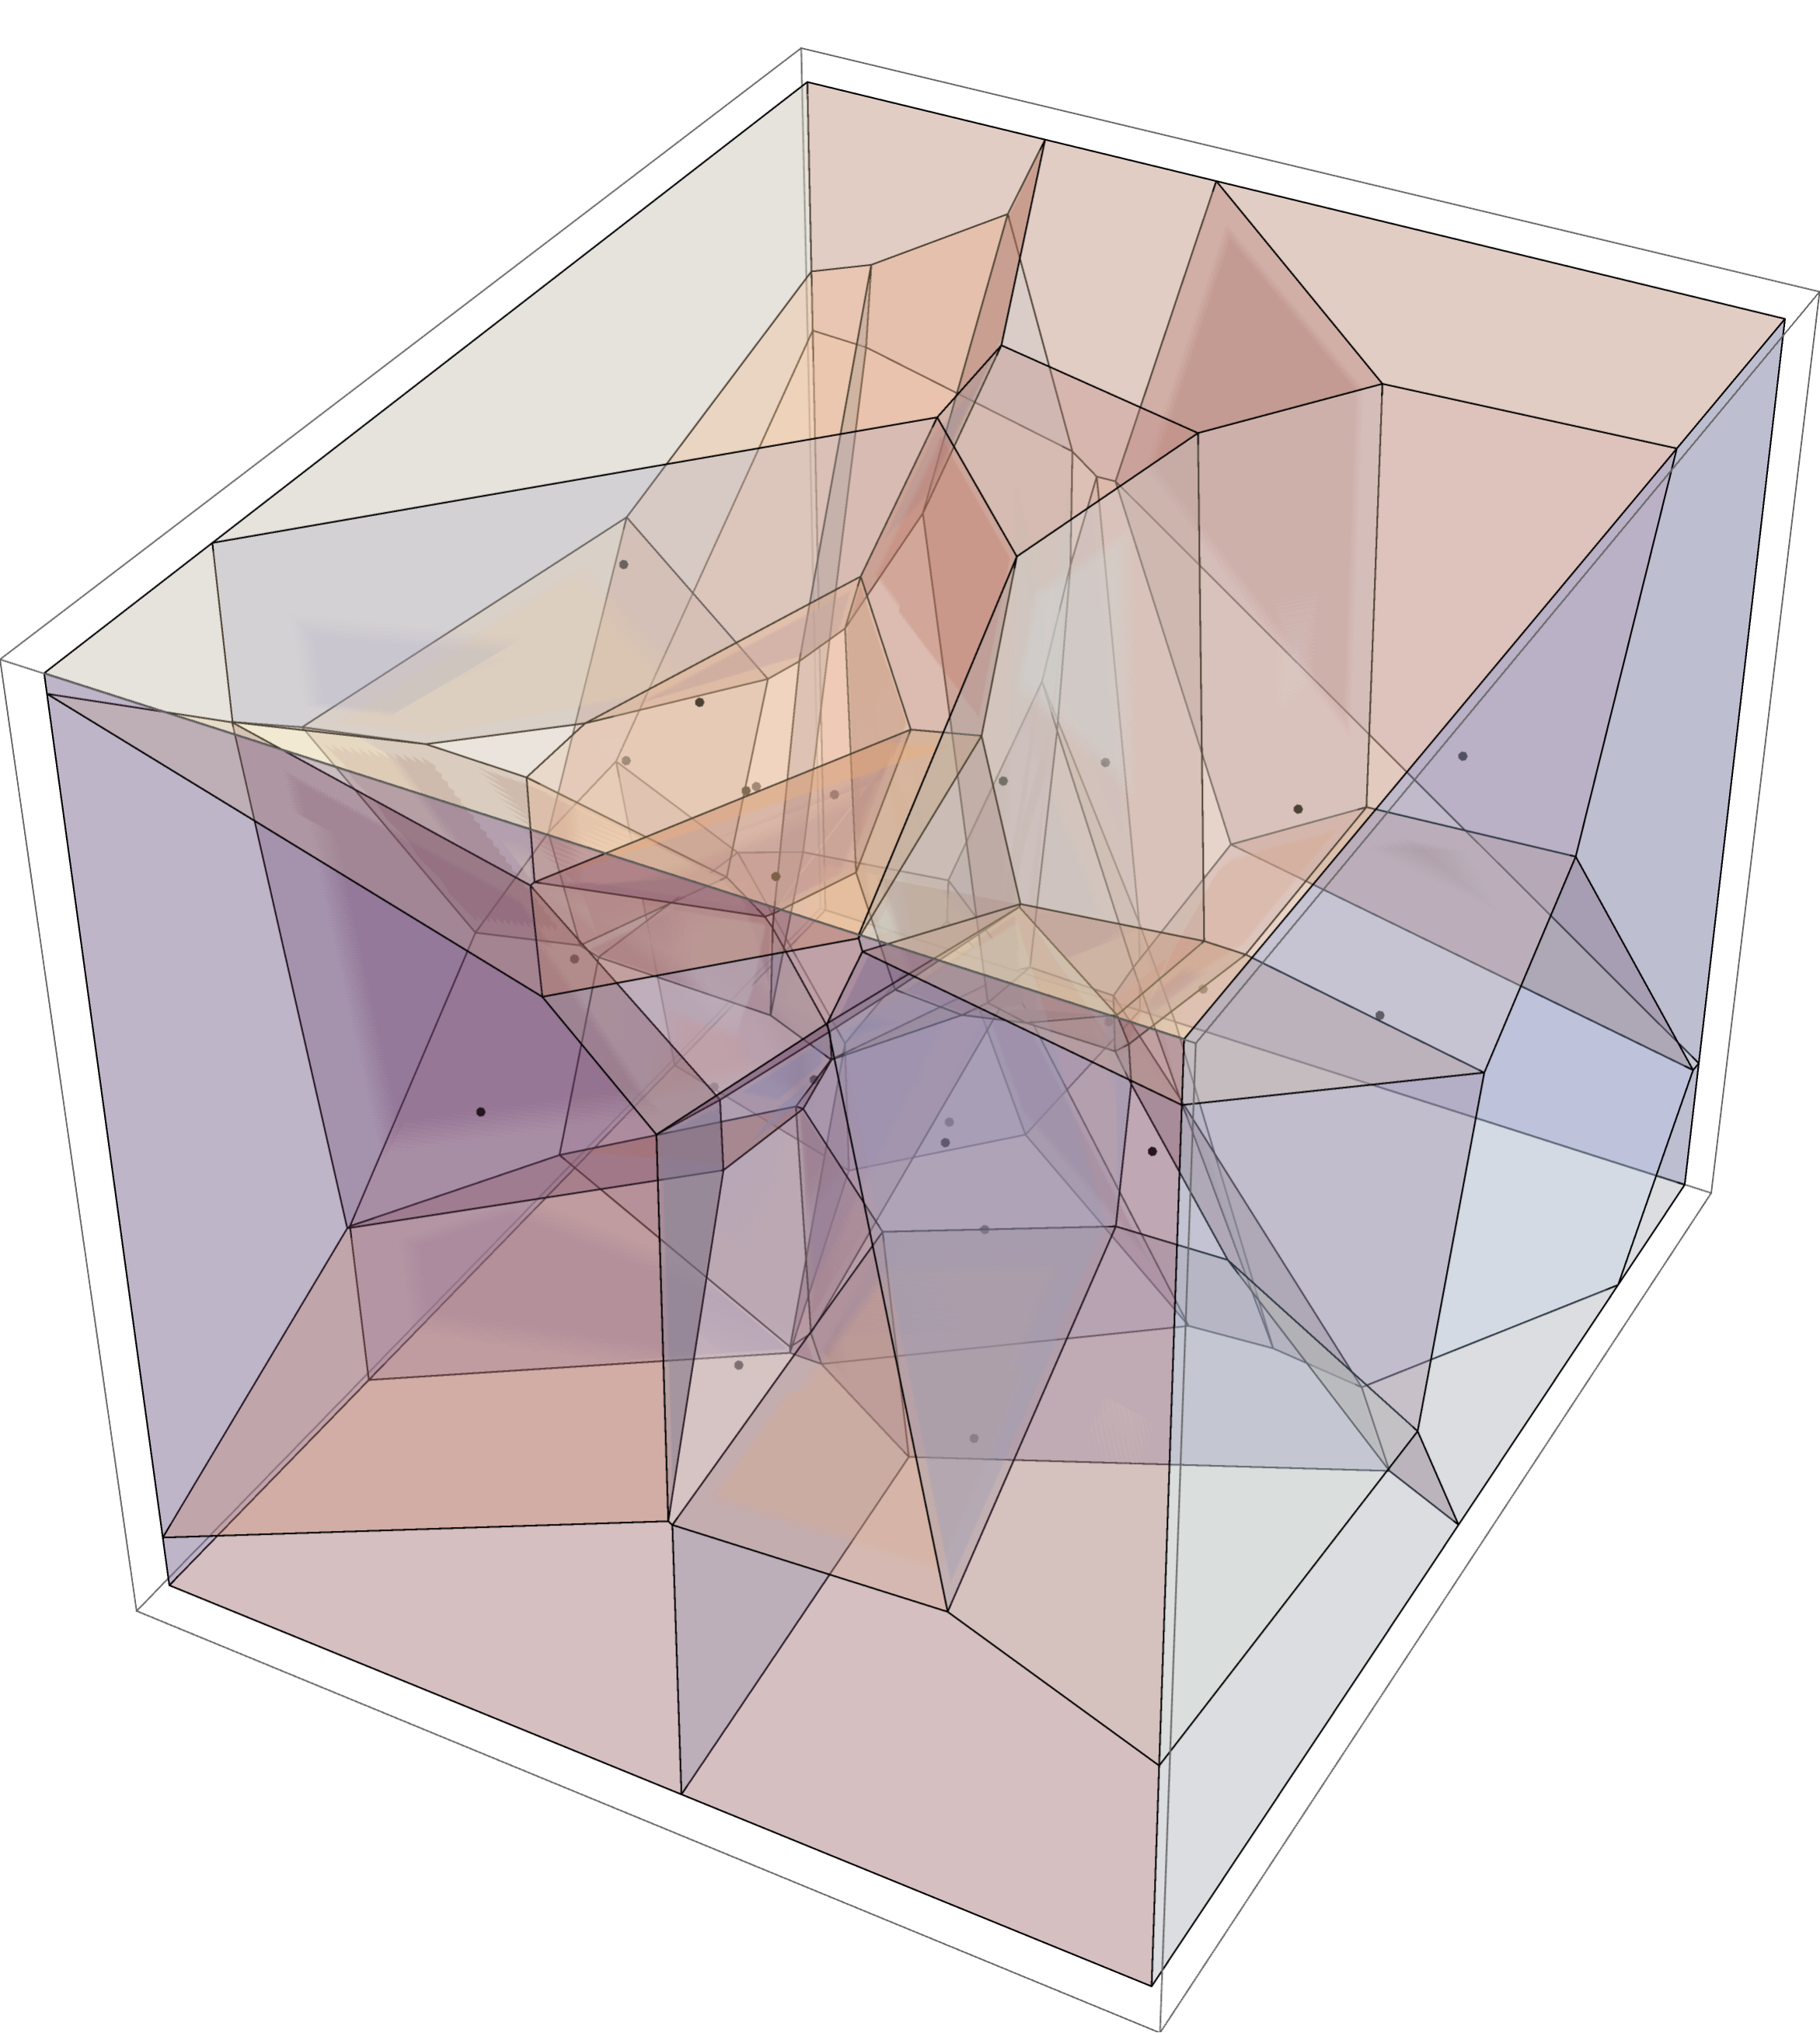
\includegraphics[width=0.48\textwidth, height=0.48\textwidth]{./fig/diagrams/Euclidian Voronoi diagram 3d.png}
            \label{fig:voronoi_3d}
            }
            \caption{
                (a) an example of 20 Voronoi cells in \ac{2D} \cite{Voronoi2d} (b) 25 Voronoi cells in \ac{3D} \cite{Voronoi3d}
            }
            \label{fig:voronoi_diagrams}
        \end{figure}
    
    \subsection{Additional Constraints and Modifications}
        To extend the approach to the \ac{3D} case, several adjustments are made.
        The weighting rule (\ref{eqn:beta_weighting}) remains unchanged. 
        However, in both the azimuth update rule (\ref{eqn:azimuth_2d}) and the azimuth reset rule (\ref{eqn:azimuth_reset_2d}), only the displacement of centroids projected onto the $xy$-plane is taken into account.
        The modified formulations for the \ac{3D} case are as follow:
        \begin{itemize}
            \item \textbf{Azimuth update rule \ac{3D}}
                \begin{equation}
                    \label{eqn:azimuth_3d}
                    \dot{\theta}_i = 
                    \begin{cases}
                        k  & \text{if } \theta < \frac{\pi}{2} \land \|\mathbf{c}_{\mathcal{A}_i} - \mathbf{c}_{\mathcal{S}_i}\|_{xy} > d_4 \land \|\mathbf{p}_i - \mathbf{c}_{\mathcal{A}_i}\|_{xy} > d_3 \\
                        -k & \text{if } \theta > 0 \land \neg (\|\mathbf{c}_{\mathcal{A}_i} - \mathbf{c}_{\mathcal{S}_i}\|_{xy} > d_4 \land \|\mathbf{p}_i - \mathbf{c}_{\mathcal{A}_i}\|_{xy} > d_3) \\
                        0  & \text{otherwise} \text{.}
                    \end{cases}
                \end{equation}
            \item \textbf{Azimuth reset rule \ac{3D}}
                \begin{equation}
                    \label{eqn:azimuth_reset_3d}
                    \theta = 0 \quad \text{if } \theta = \frac{\pi}{2} \land \| \mathbf{p}_i - \mathbf{\overline{c}}_{\mathcal{A}_i} \|_{xy}\text{.}
                \end{equation}
        \end{itemize}

        The notation $\| \cdot \|_{xy}$ denotes the Euclidean norm computed in the $xy$-plane only, defined as:
        \begin{equation}
            \| \mathbf{p}_i - \mathbf{p}_j \|_{xy} = \sqrt{(x_i - x_j)^2 + (y_i - y_j)^2}\text{.}
        \end{equation}

        Additionally, $Z_{clipping}$ is applied to each sensing cell $\mathcal{S}_i$, constraining it within the vertical limits defined by $\min_z$ and $\max_z$:

        \begin{equation}
            \mathcal{S}_i = \left\{\mathbf{q} \in \mathcal{Q} \mid \|\mathbf{q} - \mathbf{p}_i\| \leq r_{s,i}, \quad \min_z \leq q_z \leq \max_z \right\}\text{,}
        \end{equation}

        where $\text{min}_z$ and $\text{max}_z$ define the vertical bounds within which the sensing region $\mathcal{S}_i$ is restricted. 
        This ensures that the agent cannot exceed these limits, as it follows the computed centroid \( \mathbf{c}_{V_i} \). 
        By constraining the sensing radius, the agent remains confined within the specified region, preventing it from moving outside the vertical interval $\min_z$ to $\max_z$.

        The destination rotation rule $Z_{rule}$ is introduced to enhance agents avoidance by rotating the computed destination $\mathbf{d}_i$ by an angle $\phi$.
        For vertical rotation angle $\phi$, the following condition is intorduced
        \begin{equation}
            \label{eqn:phi_condition}
            \Omega = \|\mathbf{c}_{\mathcal{A}_i} - \mathbf{c}_{\mathcal{S}_i}\|_z < d_6 \land \|\mathbf{p}_i - \mathbf{c}_{\mathcal{A}_i}\|_z \lor 
            | \|\mathbf{p}_i - \mathbf{c}_{\mathcal{S}_i}\|_{xy} - \|\mathbf{p}_i - \mathbf{c}_{\mathcal{A}_i}\|_{xy} | > d_7 \text{.}
        \end{equation}
        This condition has two main parts, combined by a logical or. The first part evaluates the vertical displacement of the centroid of the partitioned cell $\mathbf{c}_{\mathcal{A}_i}$ from the centroid of the sensing cell $\mathbf{c}_{\mathcal{S}_i}$ and the
        displacement of the agents position $\mathbf{p}_i$ from  $\mathbf{c}_{\mathcal{A}_i}$.
        The second part considers the difference in the horizontal plane between the agent's position and the centroids $\mathbf{c}_{\mathcal{A}_i}$, $\mathbf{c}_{\mathcal{S}_i}$.

        To improve agent distriution in the vertical dimension, a directional influence on vertical exploration is introduced. 
        Given that each agent's position $\mathbf{p}_i$ and final goal $\mathbf{g}_i$, are known, this directional influence can be included into the update rule for $\phi_i$.

        First, the global heading angle, $\theta_{goal}$, towards the goal is calculated: 
        \begin{equation}
            \theta_{goal} = \text{atan2}(g_{i,y} - p_{i,y}, g_{i,x} - p_{i,x})\text{,}
        \end{equation}
        where $\mathbf{g}_{i, x}$, $\mathbf{g}_{i, y}$ represent the x and y coordinates of the goal, and $\mathbf{p}_{i, x}$, $\mathbf{p}_{i, y}$ represent the x and y coordinates of the agent.
        The resulting angle is in the range $[-\pi, \pi]$.
        Next, the heading angle is linearly mapped to a direction influence $D_{\text{influence}}$ value in the range [-1, 1]:
        \begin{equation}
            D_{\text{influence}} = \frac{\theta_{goal}}{\pi}\text{.}
        \end{equation}
        This mapping ensures that agents traveling directly northward (from South to North) have a directional influence close to one, that will promote upward vertical exploration. 
        Similarly, agents traveling southward have a direction influence close to -1, promoting downward exploration. 
        Agents moving primarily eastward or westward have a directional influence close to 0, resulting in minimal vertical exploration.
        This strategy encourages a more uniform distribution of agents throughout the \ac{3D} space. 

        To determine the adjustment to the agent's vertical orientation, the directional influence $D_{\text{influence}}$ is combined with the relative vertical displacement of the agent and $\mathbf{c}_{\mathcal{S}_i}$
        Weighted average is used to combine them: 
        \begin{equation}
            \label{eqn:combined_influace}
            C_{\text{influence}} = \frac{w_1 \cdot (\mathbf{c}_{\mathcal{S}_i,z} - \mathbf{p}_{i,z}) + w_2 \cdot D_{influence}}{w_1 + w_2}\text{,}
        \end{equation} 
        where $w_1$ $w_2$ are weighting factors. The resulting combined influence $C_{\text{influence}}$ is then used to update the agent's rotation of it's destination $\mathbf{d}_i$ by $\phi_i$.

        Based on condition \eqref{eqn:phi_condition} and \eqref{eqn:combined_influace} update rule for $\phi_i$ can be constructed as follows:
        \begin{equation}
            \label{eqn:phi_update}
            \dot{\phi}_i = 
            \begin{cases}
                k  & \text{if } \phi_i < \frac{\pi}{4} > \land C_{\text{influence}} > 0 \land \Omega \\
                0  & \text{if } \phi_i > \frac{\pi}{4} > \land C_{\text{influence}} > 0 \land \Omega \\
                -k & \text{if } \phi_i > -\frac{\pi}{4} > \land C_{\text{influence}} \leq 0 \land \Omega \\
                0  & \text{if } \phi_i < -\frac{\pi}{4} > \land C_{\text{influence}} \leq 0 \land \Omega \\
                -k & \text{if } \phi_i > 0 \land \neg \Omega \\
                k  & \text{if } \phi_i < 0 \land \neg \Omega \\
                0  & \text{otherwise}\text{,}
            \end{cases}
        \end{equation}
        where the first four cases control the rotation of the agent's destination $\mathbf{d}_i$ and the final three cases handle the smooth convergence of $\phi_i$ back to 0, when the condition $\Omega$ is not met. 

        After the application of the rules for $\theta_i$ and $\phi_i$, the agent's destination is updated as:
        \begin{equation}
            \label{eqn:destination_update}
            \mathbf{d}_i =
            \begin{pmatrix}
                p_{i,x} +  \|\mathbf{p}_i - \mathbf{g}_i\| \cdot \sin(\phi_{\mathbf{g}_i} + \phi_i) \cdot \cos(\theta_{\mathbf{g}_i} - \theta_i) \\
                p_{i,y} + \|\mathbf{p}_i - \mathbf{g}_i\| \cdot \sin(\phi_{\mathbf{g}_i} + \phi_i) \cdot \sin(\theta_{\mathbf{g}_i} - \theta_i) \\
                p_{i,z} + \|\mathbf{p}_i - \mathbf{g}_i\| \cdot \cos(\phi_{\mathbf{g}_i} + \phi_i)
            \end{pmatrix}\text{,}
        \end{equation}

        where $\phi_{\mathbf{g}_i} = \arccos(\frac{\mathbf{g}_{i,z} - \mathbf{p}_{i,z}}{\|\mathbf{p}_i - \mathbf{g}_i\|})$ is the polar angle from z-axis to the goal, 
        $\theta_{\mathbf{g}_i} = atan2( \mathbf{g}_{i,y} - \mathbf{p}_{i,y}, \mathbf{g}_{i,x} - \mathbf{p}_{i,x})$ is the azimuthal angle in the xy-plane to the goal.
    
    \subsection{Algorithm Walkthrough}
        At each iteration, the proposed algorithm performs a sequence of actions to control agent movement. 
        These actions can be summarized as follows:
        \begin{enumerate}
            \item \textbf{Cell Generation:} \\
                For each agent, two cells are generated: a partitioned cell, denoted as $\mathcal{A}$ and a sensing cell, denoted as $\mathcal{S}$.
            \item \textbf{Centroid Computation:}
                \begin{itemize}
                    \item The centroid of cell $\mathcal{A}$, $c_{\mathcal{A}}$ is computed using a weighted function that considers both the agent's goal position, $\mathbf{g}_i$, and its current destination, $\mathbf{d}_i$.
                    \item The centroid of cell $\mathcal{S}$, $c_{\mathcal{S}}$ is computed using a weighted function that considers only the agent's current destination, $\mathbf{d}_i$.
                \end{itemize}
            \item \textbf{Rule Application and Destination Update:} \\
                A set of rules is applied to: 
                \begin{itemize}
                    \item Adjust weighting function usied in the centroid computations \eqref{eqn:beta_weighting}.
                    \item Rules to update $\theta_i$ \eqref{eqn:azimuth_3d} and $\phi_i$ \eqref{eqn:phi_update} are applied.
                    \item Update the agent's destination $\mathbf{d}_i$ \eqref{eqn:destination_update}.
                \end{itemize}
            \item \textbf{Agent movement} \\
                Finally, the agent is directed towards a centroid location $c_{\mathcal{A}}$.
        \end{enumerate}
        This process is repeated until all agents reach their goals.

        

\section{Simulation and Results Analysis}

    \subsection{Computational Implementation Details}
        The continuous algorithm presented in the previous section can be easily discretized for implementation in a computational enviroment.
        Instead of continuous sets, the cells $\mathcal{A}$ and $\mathcal{S}$ are aproximated using a set of discrete points.   
        Discrete points are partitioned out when definition \eqref{eq:voronoi_cell_account_encum} is not met.
        \begin{figure}[H]
            \centering
            \subfloat[Example of discretized cells ($\mathcal{A} = \mathcal{S}$)] {
            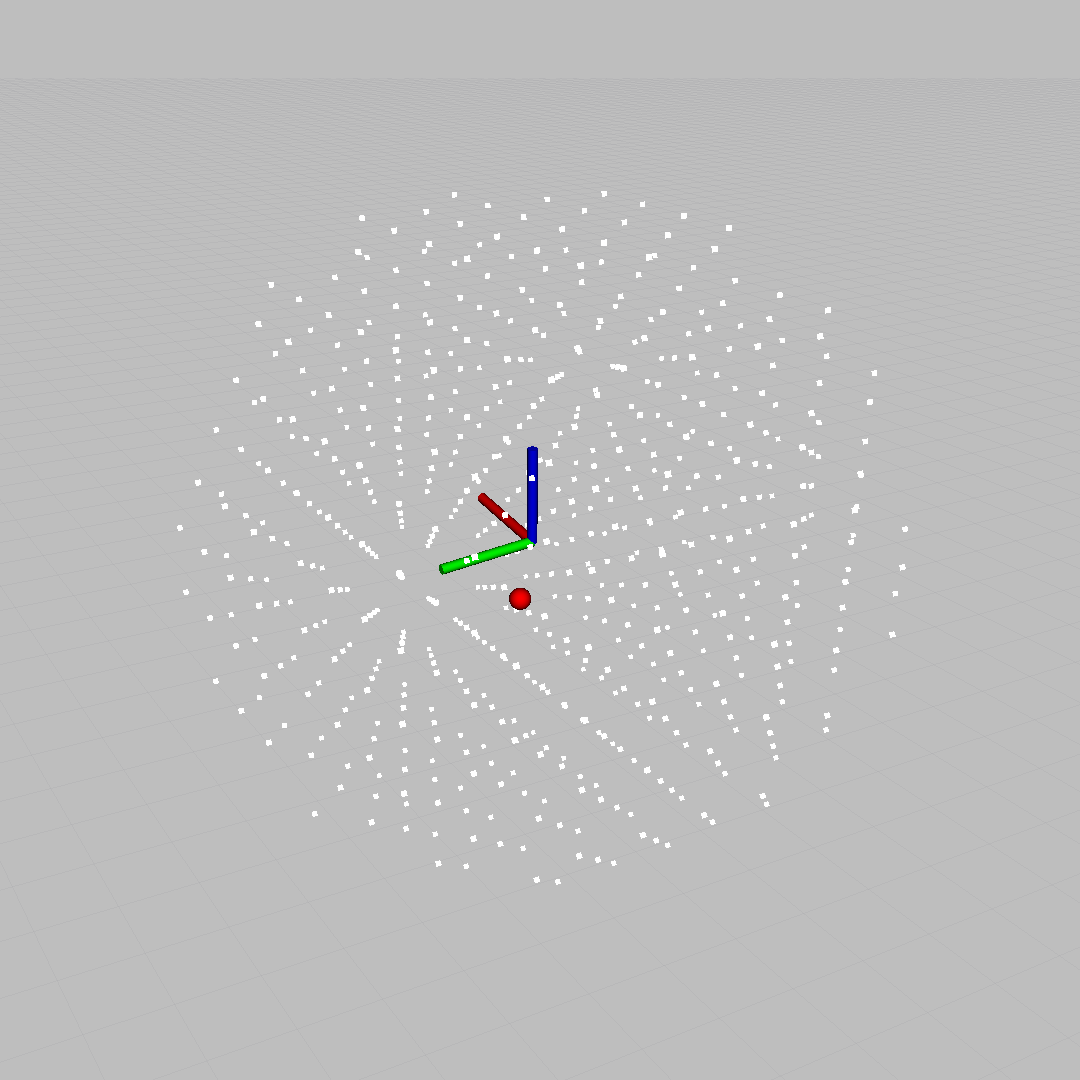
\includegraphics[width=0.48\textwidth, height=0.48\textwidth]{./fig/rviz/cs_equal_ca.png}
            \label{fig:rviz_cs_eq_ca}
            }
            \subfloat[Example of a partitioned cell $\mathcal{A}$] {
            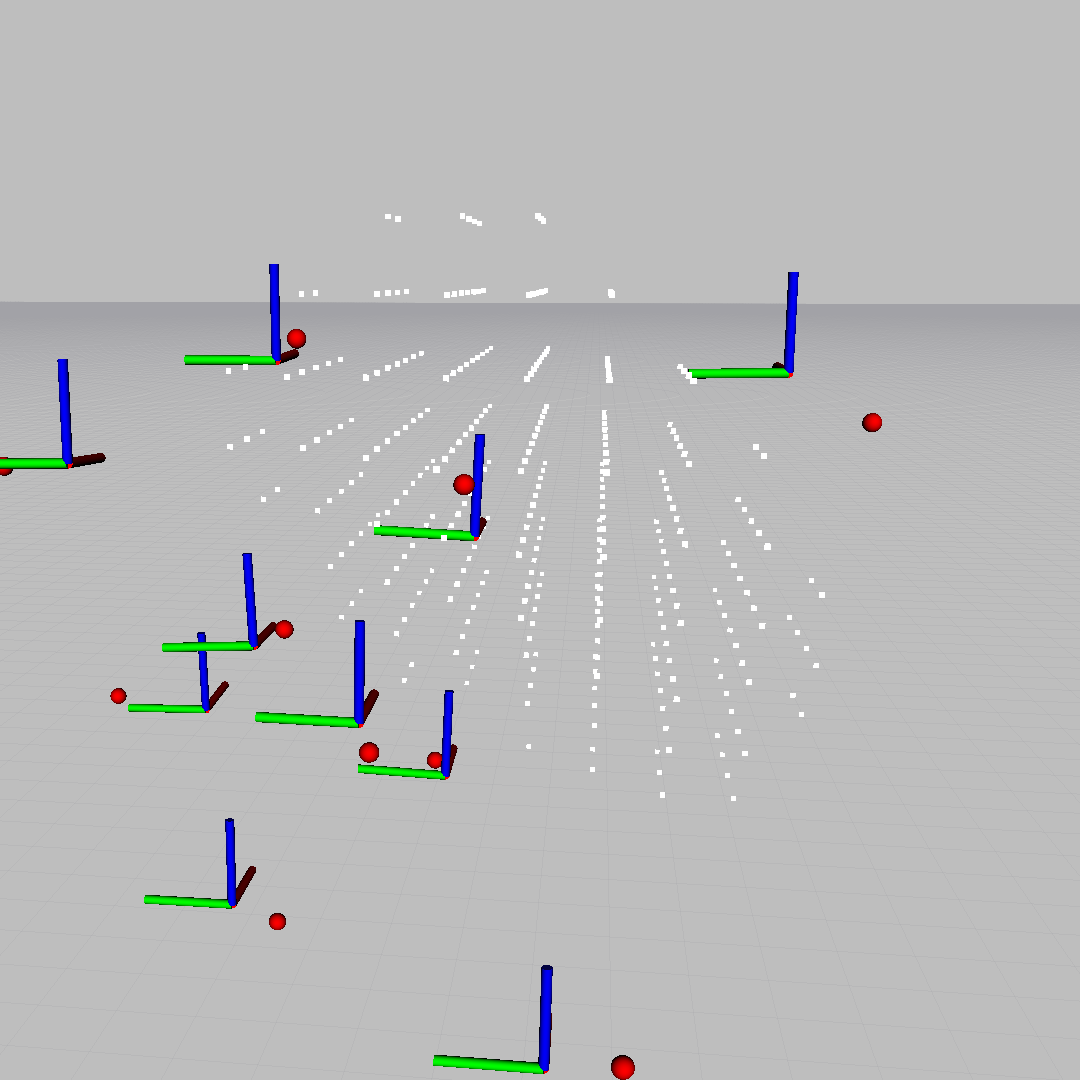
\includegraphics[width=0.48\textwidth, height=0.48\textwidth]{./fig/rviz/ca_partitioned.png}
            \label{fig:rviz_ca_partitioned}
            }
            \caption{
                Discrete approximation of Voronoi cells, with centroid $c_{\mathcal{A}}$ shown as a red dot.(a) Example where the partitioned cell $\mathcal{A}$ and the sensing cell $\mathcal{S}$ are the same. (b) Example where the partitioned cell $\mathcal{A}$ is partitioned by other \ac{UAV}s.
            }
            \label{fig:rviz_cells}
        \end{figure}
        
    \subsection{Simulation Enviroment}
        In this simulation, the term 'agent' refers to the \ac{UAV}, which were simulated using the framework provided by \ac{MRS} \cite{mrs_uav_system}.
        Each \ac{UAV} obtains its global ground truth position from the ROS simulator.
        The positions of neighboring \ac{UAV}s were estimated using simulated blinking ultraviolet markers, following the method described in \cite{uvdd1} and \cite{uvdar_package}.
        The following constraints are relevant for each \ac{UAV}:
        \begin{table}[h]
            \centering
            \renewcommand{\arraystretch}{1.1}
            \begin{tabular}{|l|c|}
                \hline
                \textbf{Parameter} & \textbf{Value} \\ \hline
                    Maximal horizontal velocity [\SI{}{\meter\per\second}] & 4.0 \\ \hline
                    Horizontal acceleration [\SI{}{\meter\per\second\squared}] & 2.0 \\ \hline
                    Maximal ascending velocity [\SI{}{\meter\per\second}] & 2.0 \\ \hline
                    Vertical ascending acceleration [\SI{}{\meter\per\second\squared}] & 1.0 \\ \hline
                    Maximal descending velocity [\SI{}{\meter\per\second}] & 2.0 \\ \hline
                    Vertical descending acceleration [\SI{}{\meter\per\second\squared}] & 1.0 \\ \hline
                \end{tabular}
                \caption{Motion constraints of the \ac{UAV}.}
            \label{tab:uav_constraints}
        \end{table}
        
    \subsection{Simulation Scenarios}
        To evaluate the safety and performance of the \ac{UAV}s during interactions, a series of experiments was conducted. 
        Experiments were performed primarily using circular formations, with \ac{UAV} counts of N = 5, 10, and 15. 
        Each of these circular formation experiments was repeated 10 times.
        Additionally, to extend the analysis to \ac{3D} and assess the algorithm's performance, a set of spherical formation experiments was conducted with N = 10, also repeated 10 times.
        After each \ac{UAV} was flown from the ground to its starting position, the \ac{RBL} algorithm was activated.    

        These formations provide a controlled enviroment compared to random initial position and goal locations. 
        In both circular and spherical formations, the \ac{UAV}s were evenly distributed along the circle or the surface of the sphere, with the goal position located on the opposite side.
        The radius of both circle and the sphere was set to 5 meters.
        
        The following metrics were measured across the 10 repetitions of each experiment, along with their standard deviations: success rate \( SR \ [\%] \), average trajectory length \( \overline{L} \ [\mathrm{m}] \), 
        average time to reach the goal \( \overline{t} \ [\mathrm{s}] \), average of the maximal time for \ac{UAV} to reach the goal \( \overline{t}_{\text{max}} \ [\mathrm{s}] \), and average velocity \( \overline{v} \ [\mathrm{m/s}] \).

        The specific values of the parameters used in the experiments are summarized in following table \ref{tab:experiment_parameters}:
        \begin{table}[H]
            \centering
            \caption{Parameters Used in Experiments}
            \begin{tabular}{|l|l|}
                \hline
                Parameter & Value \\
                \hline
                \hline
                Sensing radius $r_s$ [m] & 3.5 \\ \hline
                Update rate [Hz] & 10 \\ \hline
                Encumbrance $\delta_i$ [m] & 0.5 \\ \hline
                $d_1 = d_3 = d_5$ [m] & 0.5 \\ \hline
                $d_2 = d_4 = d_6$ [m] & 1.0 \\ \hline
                $d_7$ [m] & 0.2  \\ \hline
                $\min_z$ [m] & 1.0 \\ \hline
                $\max_z$ [m] & 10.0 \\ \hline
                $\beta_i^D$ [ ] & 1.5  \\ \hline
                $\eta$ [ ] & 0.9  \\ \hline
                $w_1$ [ ] & 0.7 \\ \hline
                $w_2$ [ ] & 0.3 \\ \hline

            \end{tabular}
            \label{tab:experiment_parameters}
        \end{table}

    \subsection{Experimental Results}
        \begin{itemize}
            \item \textbf{$N = 5$ Circular Formation:}
                \begin{table}[H]
                    \centering
                    \renewcommand{\arraystretch}{1.2}
                    \begin{tabular}{|l|c|c|c|c|c|}
                    \hline
                                                & \( SR \ [\%] \) & \( \overline{L} \ [\mathrm{m}] \) & \( \overline{t} \ [\mathrm{s}] \) & \( \overline{t}_{\text{max}} \ [\mathrm{s}] \) & \( \overline{v} \ [\mathrm{m/s}] \)     \\ \hline
                    RBL \ac{2D}                      & 100.00          & 21.06 $\pm$ 0.10                  & 25.15 $\pm$ 0.21                  & 25.15 $\pm$ 0.19                               & 0.83 $\pm$ 0.01                         \\ \hline
                    RBL \ac{3D}                      & 100.00          & 20.77 $\pm$ 0.29                  & 26.04 $\pm$ 0.51                  & 26.79 $\pm$ 0.27                               & 0.79 $\pm$ 0.02                         \\ \hline
                    RBL \ac{3D}\(_{\text{clipped}}\) & 100.00          & 20.60 $\pm$ 0.24                  & 26.73 $\pm$ 0.47                  & 27.39 $\pm$ 0.28                               & 0.77 $\pm$ 0.02                         \\ \hline
                    RBL \ac{3D}\(_z\)                & 100.00          & 20.97 $\pm$ 0.52                  & 25.54 $\pm$ 0.97                  & 26.72 $\pm$ 0.60                               & 0.81 $\pm$ 0.03                         \\ \hline
                    \end{tabular}
                \end{table}
            \item \textbf{$N = 10$ Circular Formation:}
                \begin{table}[H]
                    \centering
                    \renewcommand{\arraystretch}{1.2}
                    \begin{tabular}{|l|c|c|c|c|c|}
                    \hline
                                                & \( SR \ [\%] \) & \( \overline{L} \ [\mathrm{m}] \) & \( \overline{t} \ [\mathrm{s}] \) & \( \overline{t}_{\text{max}} \ [\mathrm{s}] \) & \( \overline{v} \ [\mathrm{m/s}] \)     \\ \hline
                    RBL \ac{2D}                      & 100.00          & 22.95 $\pm$ 1.64                  & 30.79 $\pm$ 2.28                  & 34.73 $\pm$ 0.77                               & 0.74 $\pm$ 0.07                         \\ \hline
                    RBL \ac{3D}                      & 100.00          & 22.22 $\pm$ 0.89                  & 30.05 $\pm$ 2.61                  & 34.39 $\pm$ 4.19                               & 0.73 $\pm$ 0.05                         \\ \hline
                    RBL \ac{3D}\(_{\text{clipped}}\) & 100.00          & 22.31 $\pm$ 0.69                  & 30.22 $\pm$ 1.83                  & 33.22 $\pm$ 0.93                               & 0.73 $\pm$ 0.04                         \\ \hline
                    RBL \ac{3D}\(_z\)                & 100.00          & 22.38 $\pm$ 0.88                  & 28.80 $\pm$ 2.30                  & 32.35 $\pm$ 1.25                               & 0.77 $\pm$ 0.05                         \\ \hline
                    \end{tabular}
                \end{table}
            \item \textbf{$N = 15$ Circular Formation:}
                \begin{table}[H]
                    \centering
                    \renewcommand{\arraystretch}{1.2}
                    \begin{tabular}{|l|c|c|c|c|c|}
                    \hline
                                                & \( SR \ [\%] \) & \( \overline{L} \ [\mathrm{m}] \) & \( \overline{t} \ [\mathrm{s}] \) & \( \overline{t}_{\text{max}} \ [\mathrm{s}] \) & \( \overline{v} \ [\mathrm{m/s}] \)     \\ \hline
                    RBL \ac{2D}                      & 100.00          & 23.56 $\pm$ 1.75                  & 33.89 $\pm$ 2.48                  & 38.75 $\pm$ 1.45                               & 0.69 $\pm$ 0.06                         \\ \hline
                    RBL \ac{3D}                      & 100.00          & 22.36 $\pm$ 0.97                  & 30.65 $\pm$ 3.07                  & 35.77 $\pm$ 3.72                               & 0.72 $\pm$ 0.07                         \\ \hline
                    RBL \ac{3D}\(_{\text{clipped}}\) & 100.00          & 22.32 $\pm$ 0.81                  & 30.69 $\pm$ 2.61                  & 34.50 $\pm$ 0.47                               & 0.72 $\pm$ 0.06                         \\ \hline
                    RBL \ac{3D}\(_z\)                & 100.00          & 22.64 $\pm$ 0.95                  & 29.67 $\pm$ 2.54                  & 34.27 $\pm$ 0.88                               & 0.76 $\pm$ 0.06                         \\ \hline
                    \end{tabular}
                \end{table}
            \item \textbf{$N = 10$ Spherical Formation:}
                \begin{table}[H]
                    \centering
                    \renewcommand{\arraystretch}{1.2}
                    \begin{tabular}{|l|c|c|c|c|c|}
                    \hline
                                                & \( SR \ [\%] \) & \( \overline{L} \ [\mathrm{m}] \) & \( \overline{t} \ [\mathrm{s}] \) & \( \overline{t}_{\text{max}} \ [\mathrm{s}] \) & \( \overline{v} \ [\mathrm{m/s}] \)     \\ \hline
                    RBL \ac{3D}                      & 100.00          & 14.32 $\pm$ 1.52                  & 27.76 $\pm$ 3.06                  & 32.48 $\pm$ 2.26                               & 0.51 $\pm$ 0.05                         \\ \hline
                    RBL \ac{3D}\(_z\)                & 100.00          & 14.06 $\pm$ 0.97                  & 27.17 $\pm$ 2.66                  & 31.86 $\pm$ 1.24                               & 0.55 $\pm$ 0.06                         \\ \hline
                    \end{tabular}
                \end{table}
        \end{itemize}

        The figure below visualizes the  \ac{UAV}  trajectories, showing the effect of the applied simulation rules.
        \begin{figure}[H]
            \centering
            \subfloat[Trajectories of \ac{UAV}s using 2D \ac{RBL}, $N=10$] {
                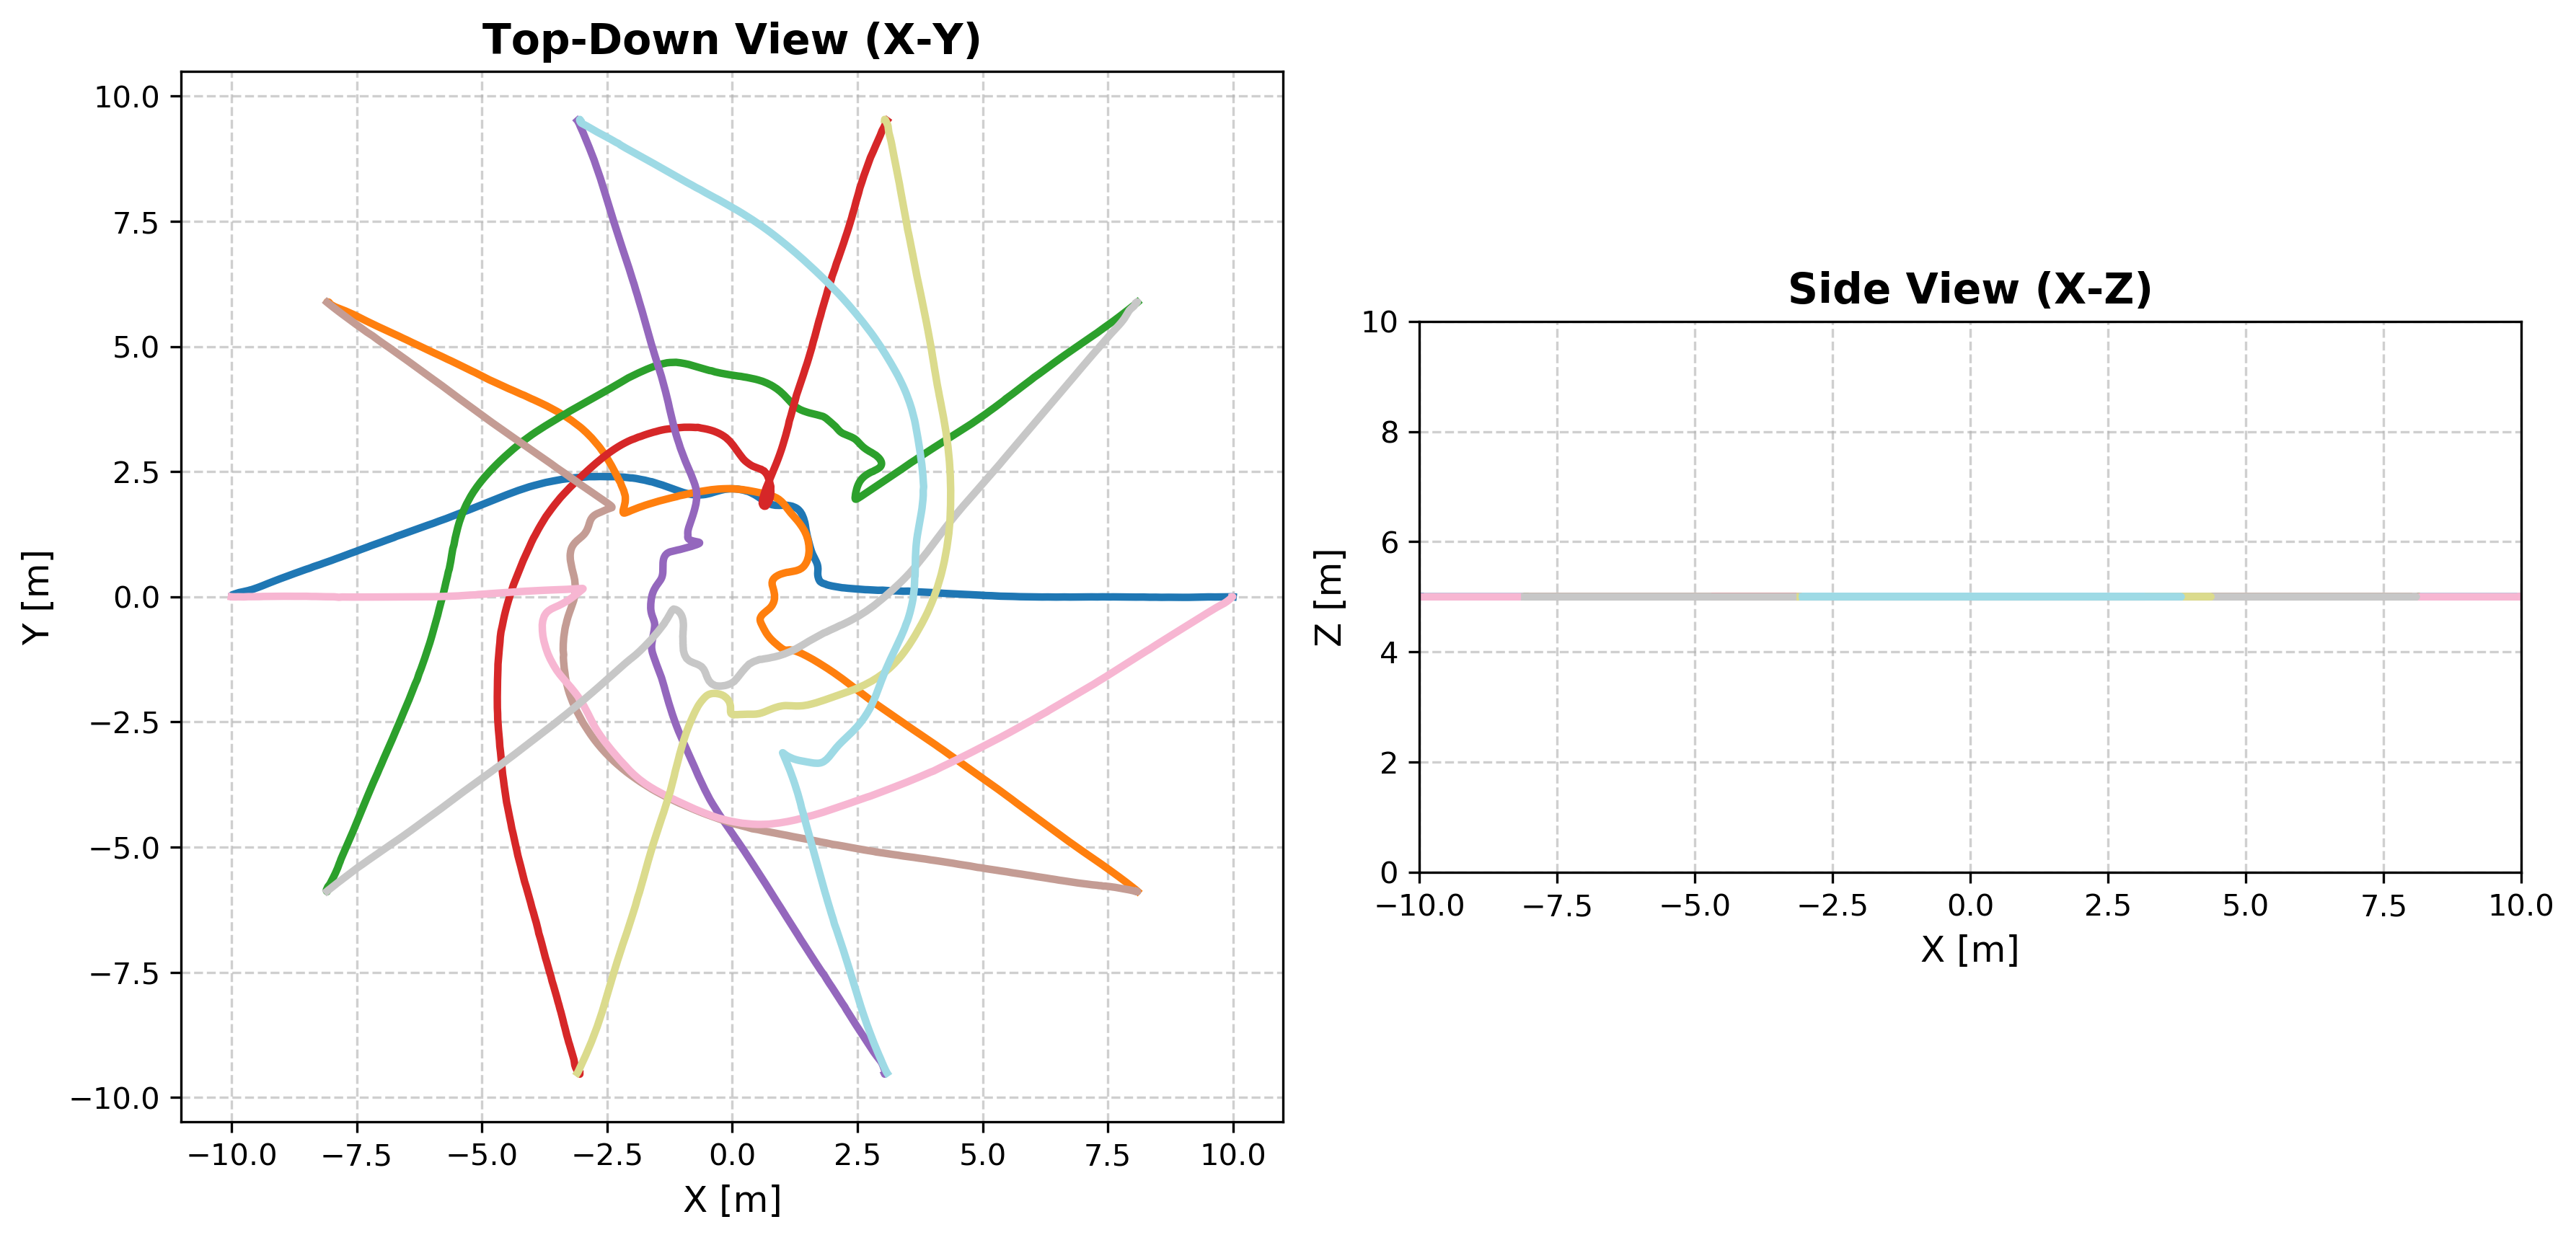
\includegraphics[width=0.48\textwidth, height=0.24\textwidth]{./fig/plots/n_10_circle_2d.png}
                \label{fig:n_10_circle_2d}
            }
            \subfloat[Trajectories of \ac{UAV}s using \ac{3D} \ac{RBL}, $N=10$] {
                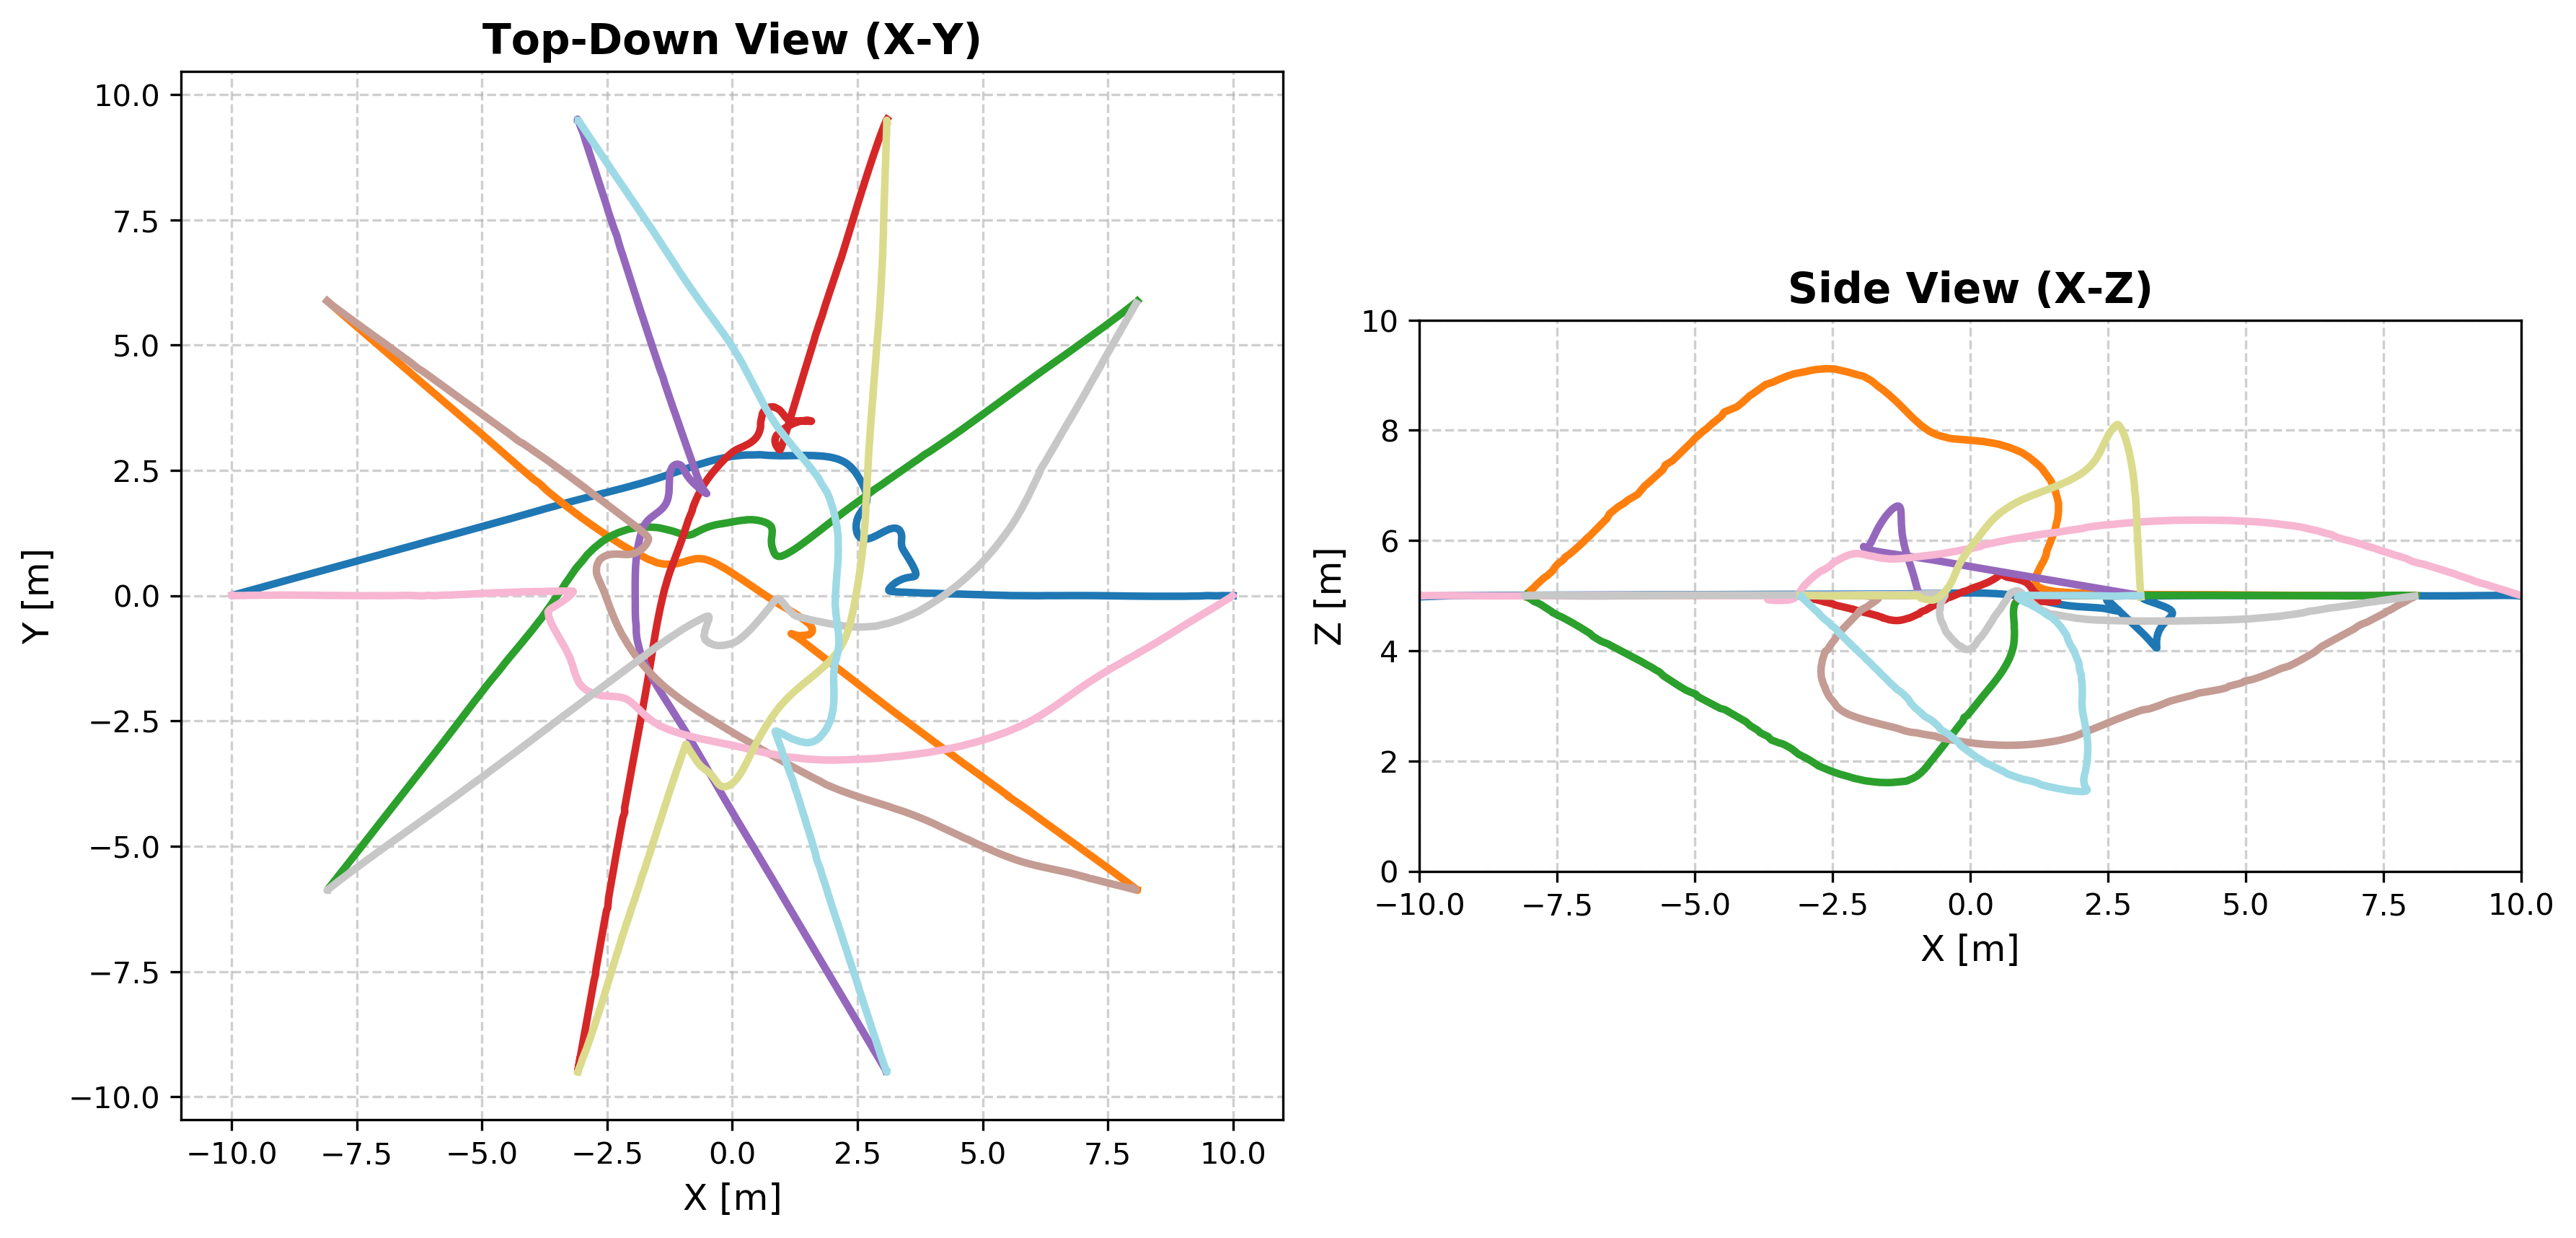
\includegraphics[width=0.48\textwidth, height=0.24\textwidth]{./fig/plots/n_10_circle_3d.png}
                \label{fig:n_10_circle_3d}
            }
            \par\medskip
            \subfloat[Trajectories of \ac{UAV}s using \ac{3D} \ac{RBL} and $Z_{clipping}$, $N=10$] {
                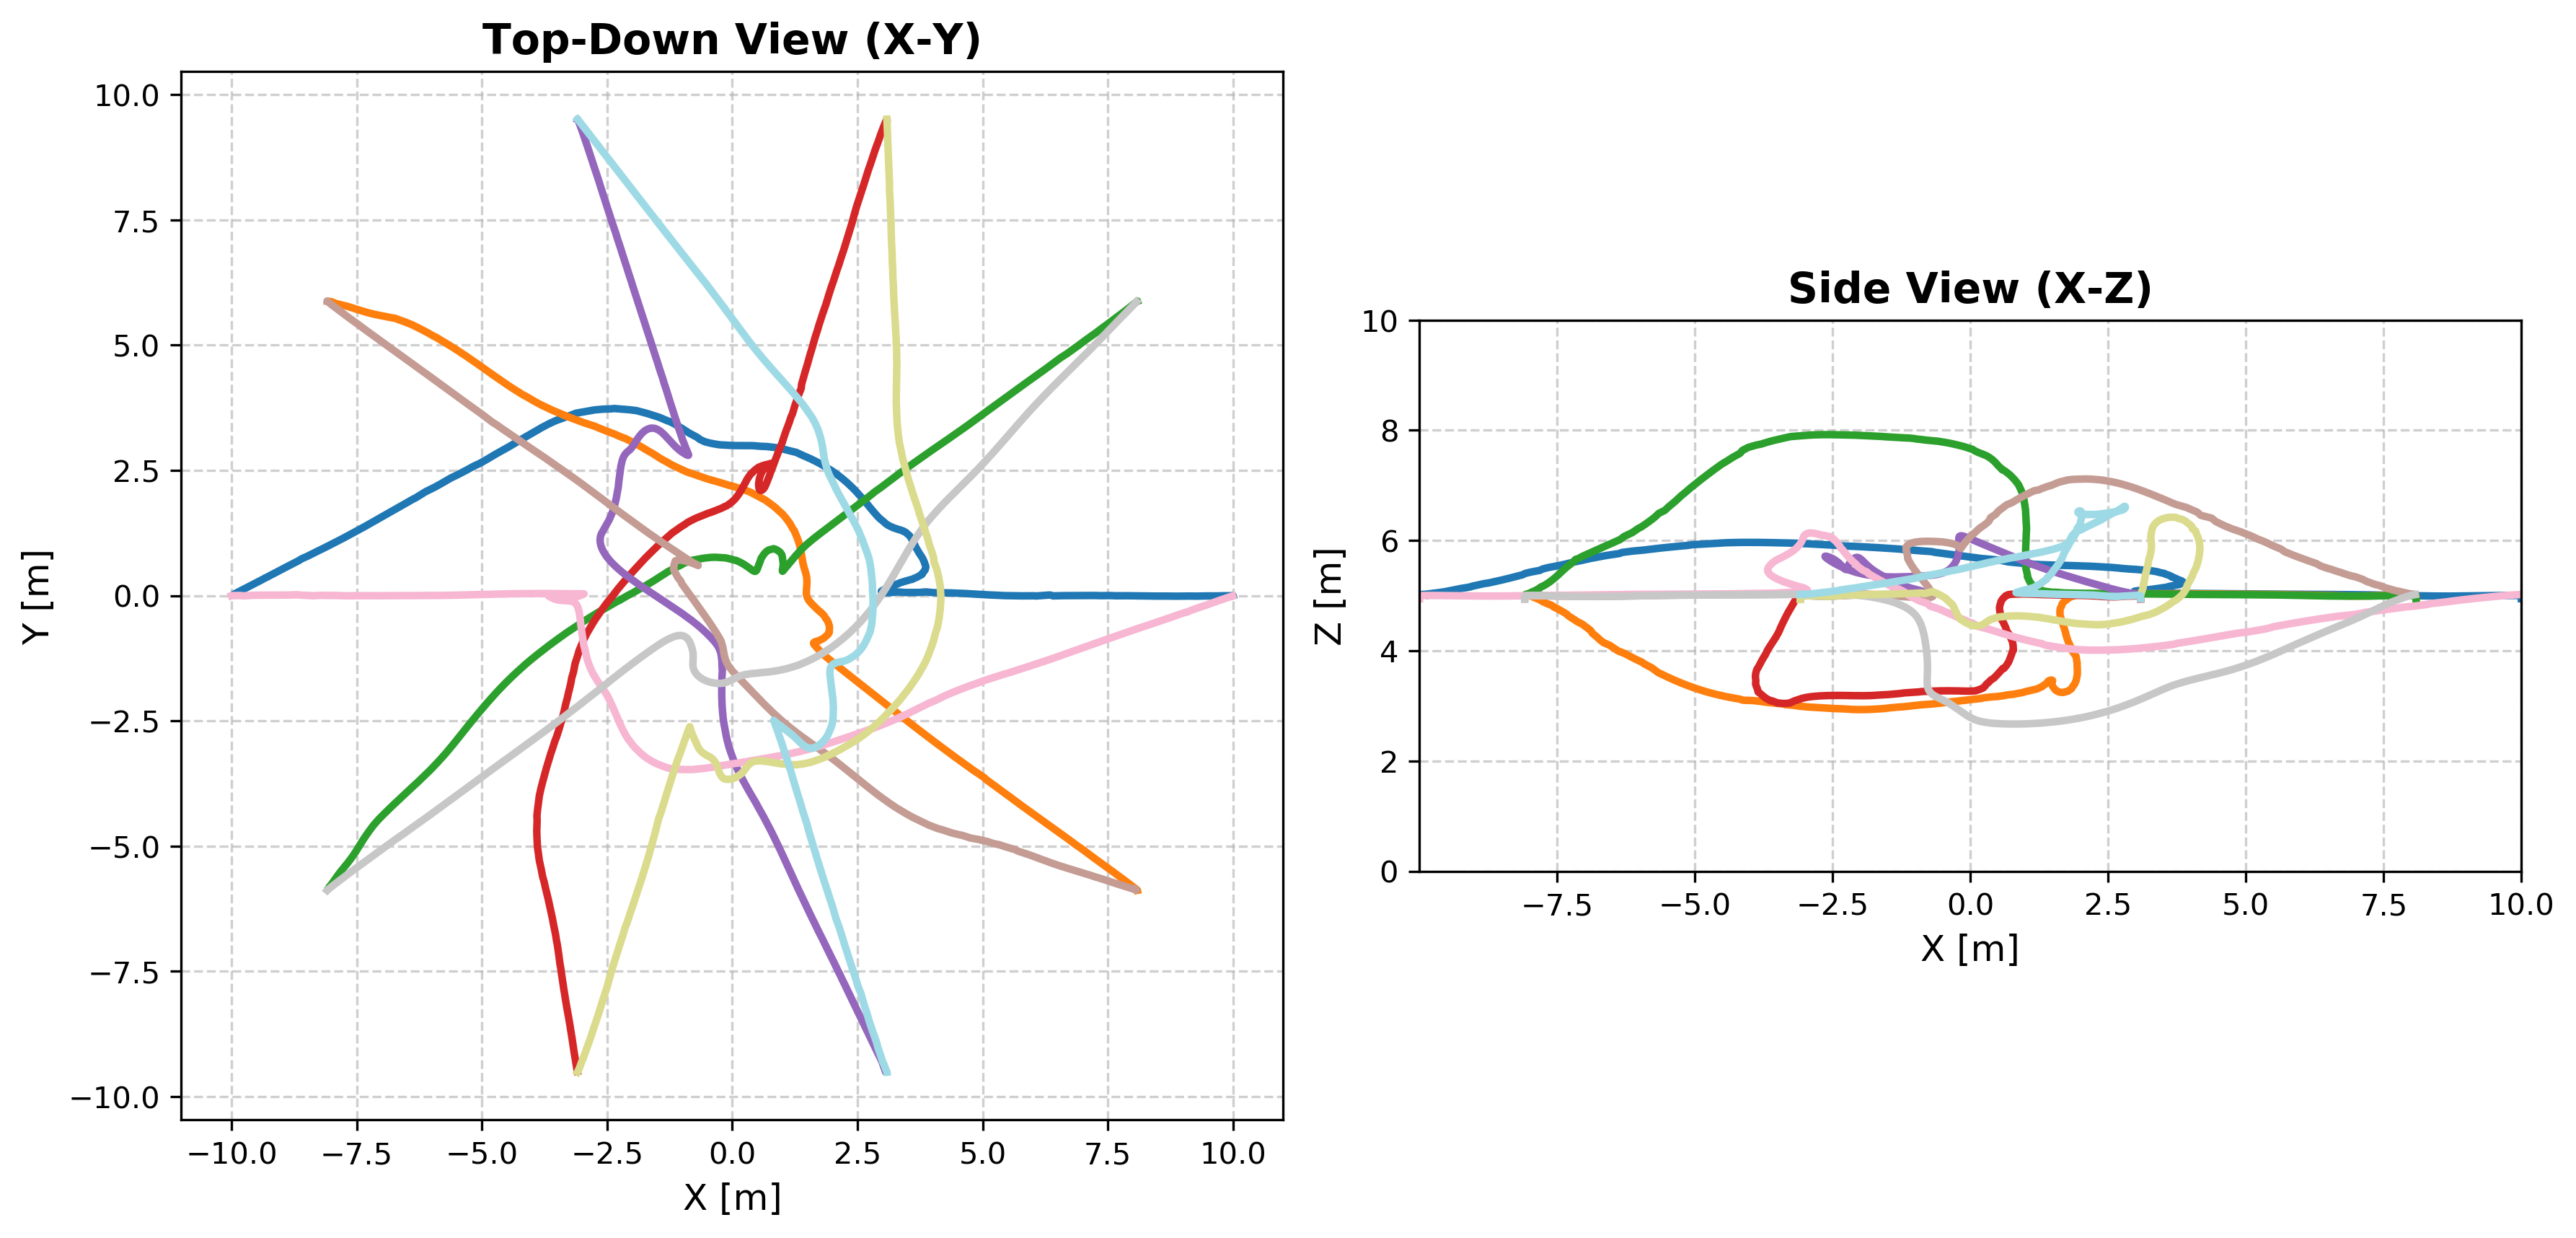
\includegraphics[width=0.48\textwidth, height=0.24\textwidth]{./fig/plots/n_10_circle_z_clipp.png}
                \label{fig:n_10_circle_z_clipp}
            }
            \subfloat[Trajectories of \ac{UAV}s using \ac{3D} \ac{RBL} and using $Z_{rule}$, $N=10$] {
                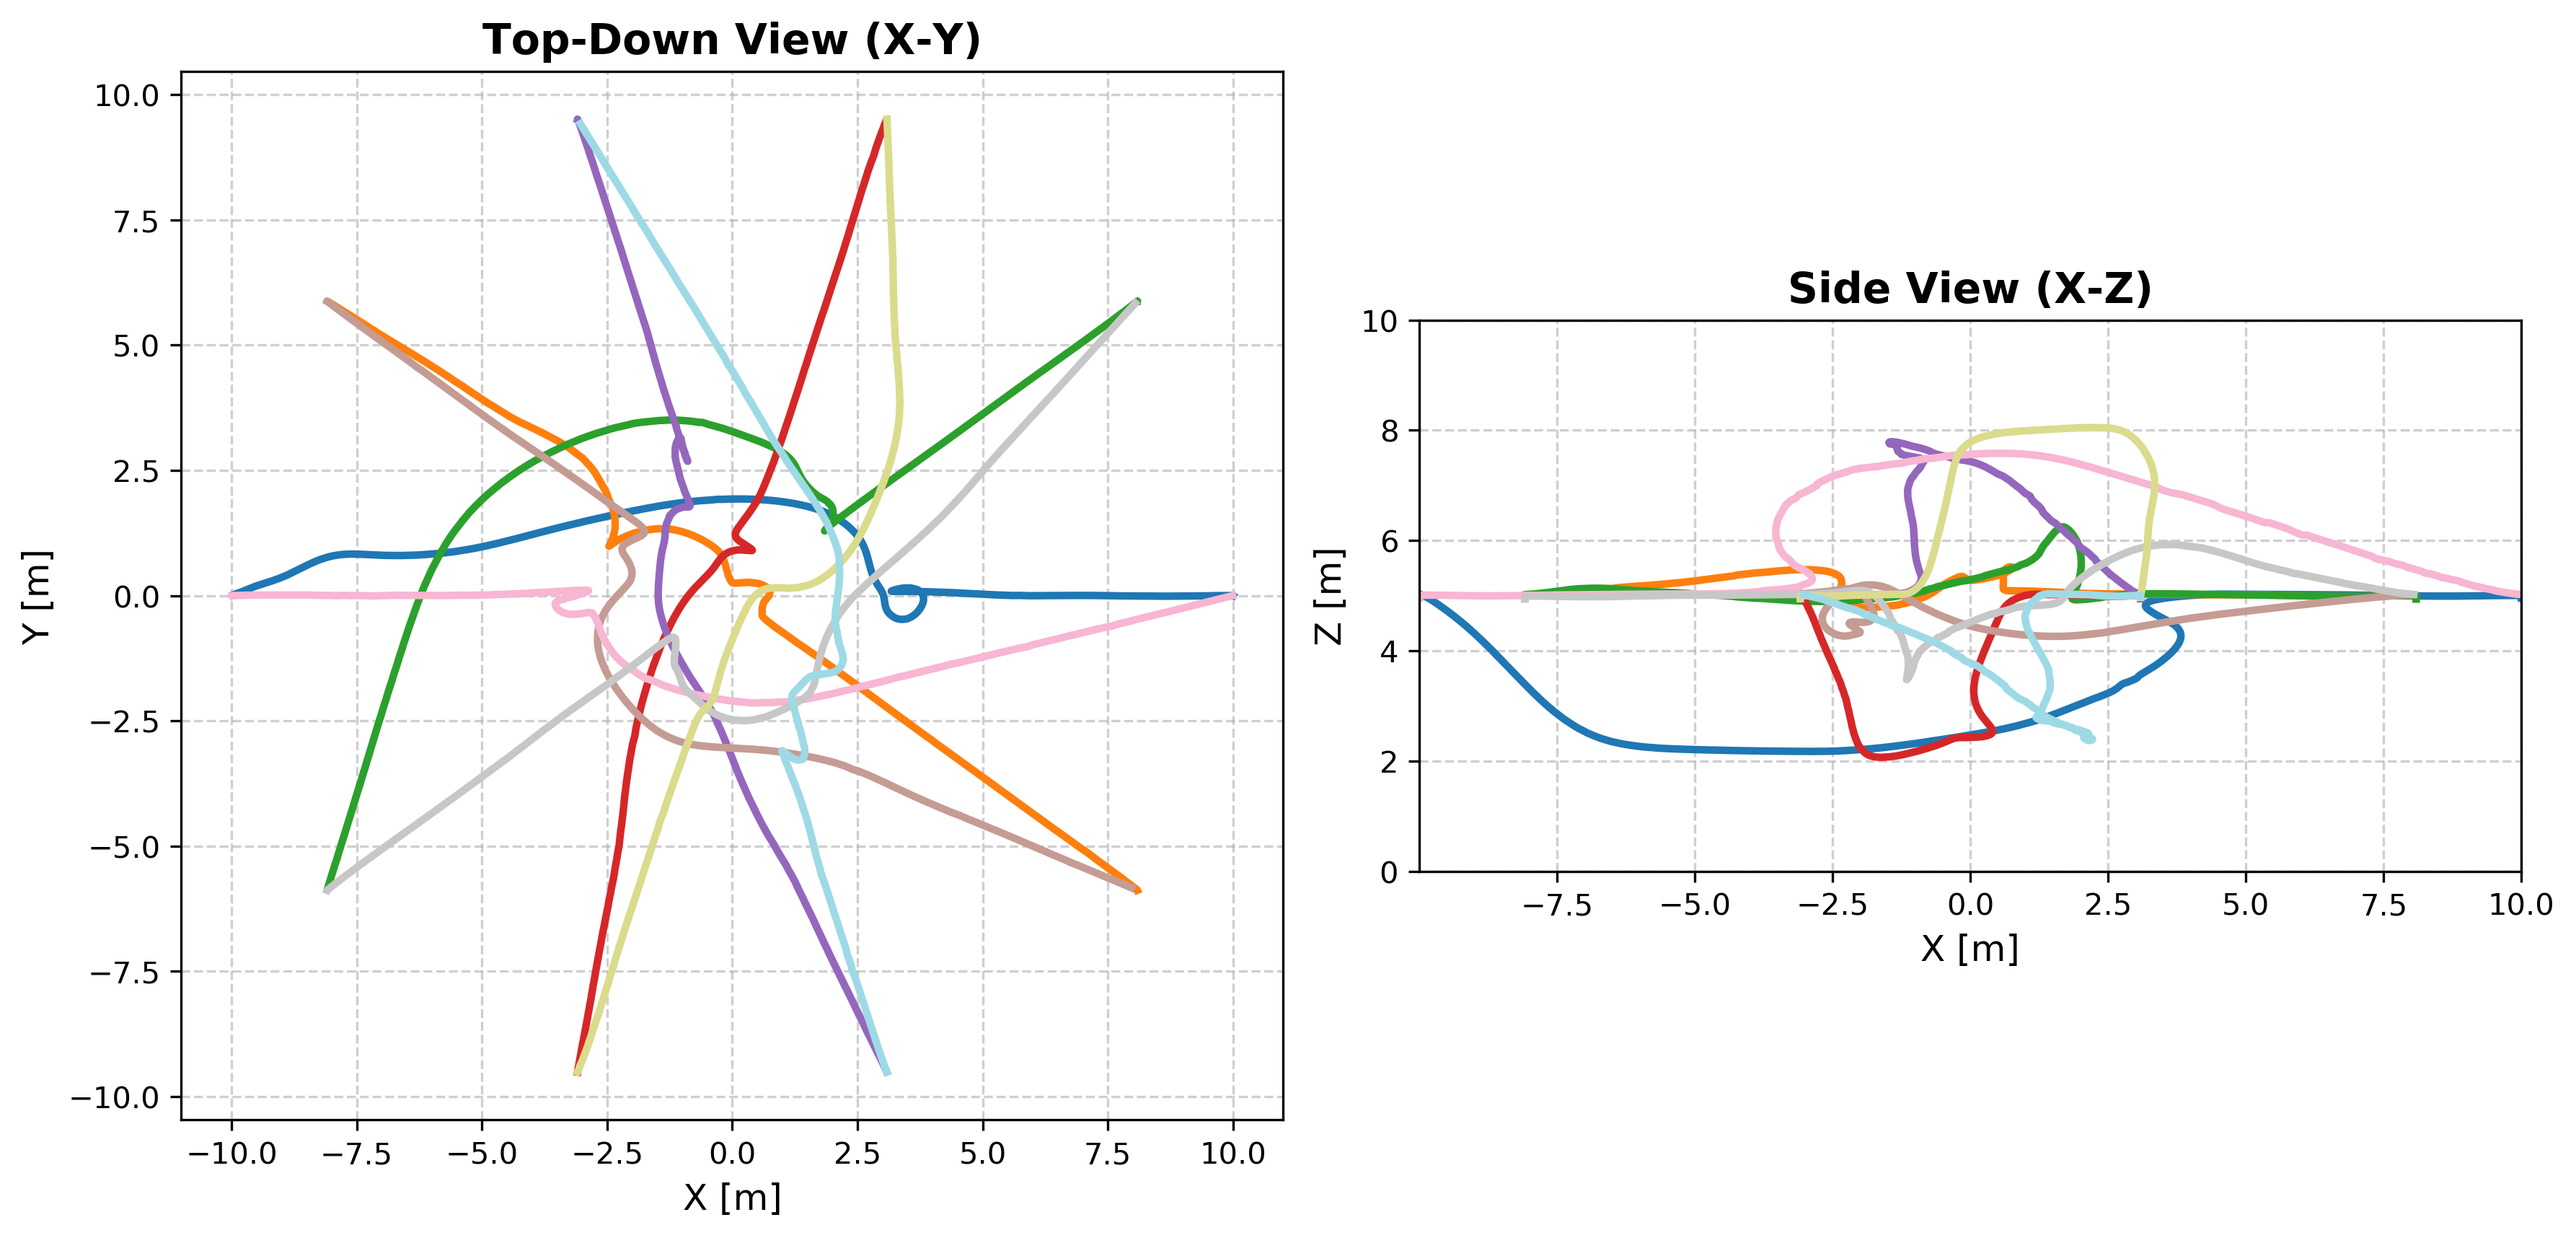
\includegraphics[width=0.48\textwidth, height=0.24\textwidth]{./fig/plots/n_10_circle_z_rule.png}
                \label{fig:n_10_circle_z_rule}
            }
            \par\medskip
            \subfloat[Trajectories of \ac{UAV}s using \ac{3D} \ac{RBL} on sphere, $N=10$] {
                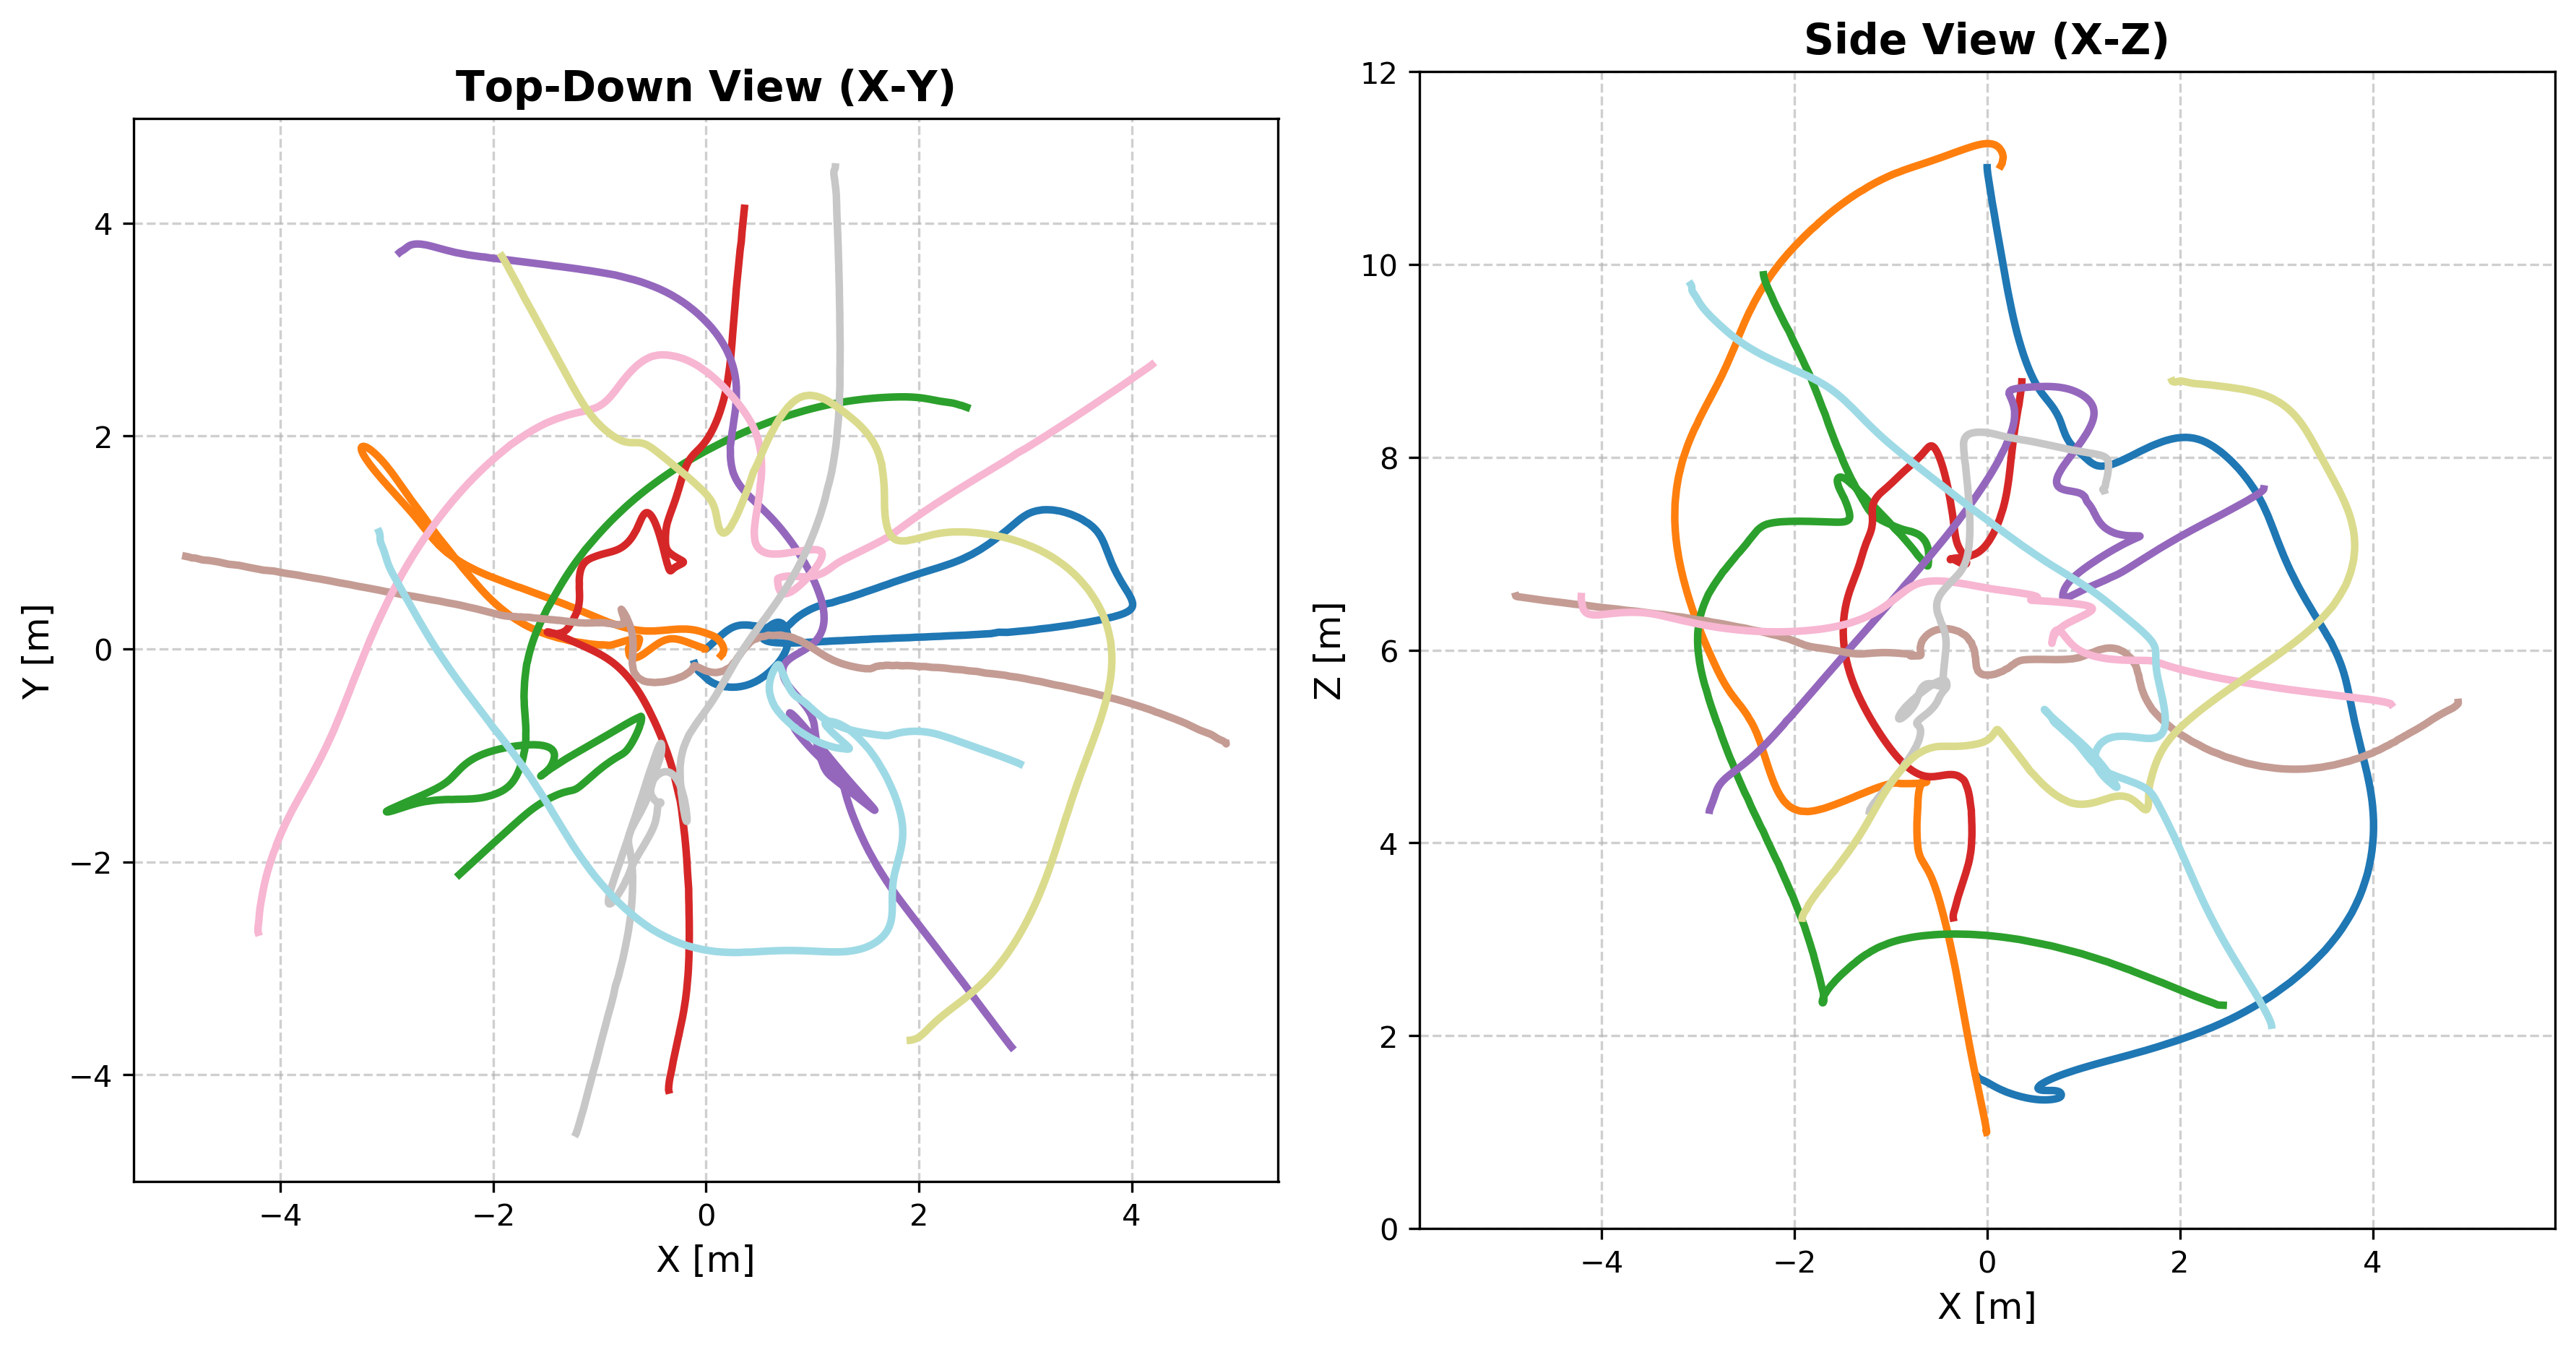
\includegraphics[width=0.48\textwidth, height=0.24\textwidth]{./fig/plots/n_10_sphere.png}
                \label{fig:n_10_sphere}
            }
            \caption{
                Visualization of UAV formations and algorithm behavior for $N=10$ (shown with top-down and side views). 
                (a) Trajectories in a \ac{2D} circular crossing. 
                (b) Trajectories in a \ac{3D} circular crossing. 
                (c) Effect of Z-axis clipping on the circular crossing. 
                (d) Effect of the Z-axis rule on the circular crossing. 
                (e) Trajectories in a \ac{3D} spherical crossing.
            }
            \label{fig:trajectories}
        \end{figure}

    \section{Comparison with State-of-the-Art Method}
        As an alternative approach developed within the MRS framework, the \ac{3D} \ac{RBL} algorithm presented here can be compared to other state-of-the-art methods like PACNav \cite{PACNav}.
        Both algorithms target communication-less UAV coordination, a feature desirable for scalability. 
        Furthermore, implementations described for both approaches have utilized UVDAR to determine the positions of neighbouring UAVs.

        A key requirement for both is some form of self-position estimation. 
        PACNav achieves this in GNSS-denied settings using SLAM techniques. 
        Similarly, \ac{RBL} can also operate without GNSS provided a robust odometry source like SLAM is available to determine the UAV's own position within a consistent frame.

        Where the approaches differ notably is in their coordination strategy. 
        PACNav utilizes a leader-follower dynamic: 'uninformed' UAVs identify and follow 'informed' (or otherwise reliable) leaders based on observed motion characteristics like path persistence and similarity, encouraging group cohesion. 
        In contrast, the RBL algorithm assigns an individual goal to each UAV. 
        Coordination emerges as each agent calculates its path based on its local modified Voronoi cell, moving towards its computed centroid while implicitly accounting for neighbours.

        Regarding validation, PACNav has demonstrated performance through real-world experiments, including navigation in a forest environment. 
        Validation of the multi-agent \ac{3D} RBL algorithm was conducted through simulation.
        The integration and experimental validation of \ac{3D} LiDAR for environmental perception and single-agent navigation within the RBL framework are addressed in the subsequent chapter.

        Another distinct approach in decentralized, communication-less coordination is the purely vision-based model presented by Mezey \cite{mezey_pure_vision}
        Unlike RBL, which relies on explicit position information, the Mezey et al. model derives control actions from a 1D visual projection field generated by detecting neighbours via onboard camera. 
        It requires no localization data. Coordination emerges from low-level visual attraction-repulsion forces, resulting in patterns like flocking or swarming rather than directed motion towards individual goals. 
        While effectively demonstrated in \ac{2D} with \ac{UGV}s, extending this purely vision-based model to complex \ac{3D} environments presents challenges regarding goal achievement. 
        Furthermore, the use of toroidal simulation environments, which mitigate group fragmentation and can facilitate specific emergent patterns like leader-follower dynamics, potentially limits the direct applicability of some observed behaviors to real-world \ac{3D} scenarios.
        The \ac{3D} RBL, by utilizing explicit position information, aims for more predictable goal-oriented navigation in \ac{3D}, although with different sensing requirements compared to the purely reactive, vision-only model of Mezey et al. 
                
    \section{Summary and Key Insights}
        This chpater detailed teh extension of \ac{RBL} algorithm, originally tested for \ac{2D} coordination, to operate in a full three-dimensional space.
        Key modification included adapting The Voronoi cell partitioning for \ac{3D}, utilizing projections for already existing azimuth update rules, and introducing a new elevation rotation angle.
        This new rule dynamically adjusts the agent's vertical destination based on relative centroid positions and directional influence towards the goal, aiming to imporve distribution.
        Note that for the directional influence to work the \ac{UAV}s need to have some sort of information about frame of reference between each other at the start of the algorithm, such as Earth's magnetic field.
        Vertical movement has also been constrained within defined interval ($\min_z$, $\max_z$).

        The proposed \ac{3D} RBL extensions were evaluated through simulations within the MRS framework, comparing performance \ac{UAV}s crossing circle and sphere. 
        The results indicate that the extension variants successfully enabled multi-agent coordination in three dimensions.
        Specifically, analysis of the simulation results reveals a trend where the performance of the \ac{3D} approach with applied rules compared to the basic \ac{2D} appears to increase with scaling number of agents. 
        For instance, based on the average completion times, the \ac{3D} variant was calculated to be aproximately 1.99\% faster than the \ac{2D} variant for N=5 agents.
        This performance is scales for larger swarms.
        For N=15 the \ac{3D} approach was calculated to be 4.22\% faster than the \ac{2D}.
        This suggests that the extension becomes increasingly beneficial in more crowded scenarios.

        While the magnitude of this observed improvement was perhaps less than initially anticipated, it is important to consider the conservative motion constraints for \ac{UAV}s on the Z-axis (velocity/acceleration), reflecting realistic \ac{UAV} dynamics but limiting vertical exploration.
        Furthermore, the parameters used for testing simulation were also conservative, suggesting that finer tuning - particularly of vertical exploration weights and weighting function agressiveness - could potentially yield better performance.
        Nonetheless, the trend indicated by these results supports the conclusion that the \ac{3D} extension effectiveness crowdeness rises.
        Furthermore, simulations in the spherical formation scenario confirmed the algorithm's capability to manage \ac{3D} navigation and coordination.

        In conclusion, the simulations presented in this chapter demonstrate the feasibility of extending the RBL algorithm to \ac{3D}. 
        The introduced elevation control rule appears particularly beneficial, enhancing the efficiency and convergence speed of the agents towards their goals in simulated \ac{3D} environments. 
        This provides a promising foundation for applying the \ac{3D} RBL algorithm to real-world UAV navigation tasks, explored further in subsequent chapter.




\chapter{UAV Navigation Using the RBL Algorithm and LiDAR Sensing\label{chap:lidar}}

    \section{Introduction}
        \subsection{Motivation}
        \ac{UAV}s are increasingly being deployed in challenging, unstructured environments like dense forests, moving beyond their traditional use in open areas.
        This shift is driven by a growing demand for autonomous solutions in sectors like environmental monitoring, forestry management (health assessment \cite{kurovec_fel_clanek}), and search and rescue, where ground-based access is difficult. 
        Furthermore, this work aligns with the broader trend of deploying \ac{UAV}s for increasingly complex tasks, such as detailed infrastructure inspection (e.g., power lines, where autonomous navigation in cluttered, potentially high \ac{EMI} environments is essential - Fly4Future \cite{f4f_powerline_inspection}). 
        Enabling \ac{UAV}s to reliably navigate point-to-point within these challenging settings is a foundational step towards realizing these advanced applications safely and efficiently.

        While the primary objective of this work is to enable successful point-to-point navigation within a forest using the \ac{RBL} algorithm, a significant secondary benefit emerges from this process. 
        By successfully navigating from point A to point B while simultaneously building a map of the traversed environment, the \ac{UAV} generates valuable spatial data about the forest structure. 
        This generated map can then serve a vital purpose: enabling enhanced planning for future missions within the same area. 
        Once a map exists, subsequent \ac{UAV} operations could potentially transition from purely reactive navigation strategies to more efficient methods with globally informed path planning. 
        Leveraging prior knowledge of obstacle locations could significantly improve efficiency of future routine tasks.
        
        \subsection{Problem Statement}
            Operating \ac{UAV}s effectively within complex, three-dimensional environments like forests presents significant navigational challenges that slow down autonomous deployment. 
            The primary problems addressed in this work originate from:
            \begin{enumerate}
                \item \textbf{\ac{GNSS}-Denied Conditions: } \\
                Within forests, the dense canopy and other obstructions frequently block or scatter \ac{GNSS} signals, leading to unreliable or completely absent reception.
                This necessitates reliance on onboard sensors and algorithms (like \ac{SLAM} based on \ac{LiDAR} and \ac{IMU} data) for accurate localization and state estimation.
                \item \textbf{Cluttered and Unpredictable Environments: } \\
                Forests are inherently cluttered with numerous static obstacles (trees, trunks, branches) and potentially dynamic ones (animals, leafs, falling branches). 
                The navigation system must be capable of perceiving these obstacles in real-time and planning safe paths around them without prior knowledge of their exact layout.
            \end{enumerate}
            Therefore, the core problem is to develop and validate a robust autonomous navigation system that allows a \ac{UAV} to reliably traverse between specified points in a cluttered, \ac{GNSS}-denied forest environment using only onboard sensing and computation.

        \subsection{Objectives}
            The primary objectives within this chapter are: 
            \begin{itemize}
                \item \textbf{Integrate the \ac{RBL} with Onboard Sensing: } \\
                    Adapt the core of the \ac{RBL} to utilize real-time sensor data. 
                    This includes modifications to sensing cell $\mathcal{S}$ due to the introduction of an anisotropic sensor. 
                    % This includes modification of sensing cell $\mathcal{S}$, because used \ac{LiDAR} doesnt see in all directions. 
                    The sensing cell needs to remain convex so the centroid computed from partitioned cell $\mathcal{A}$ remains within the set, to guarantee a safe \ac{UAV} motion.
                \item \textbf{Process Point Cloud Data: } \\
                    Implement necessary filtration to refine the raw point cloud data acquired from the \ac{LiDAR}.
                \item \textbf{Integrate external packages on the \ac{UAV}: } \\
                    Integrate and configure external software packages for simultaneous environmental mapping and robust state estimation, suitable for operation within the \ac{GNSS}-denied forest environment.
                \item \textbf{Experimental Validation: } \\
                    Conduct experiments to evaluate the performance, robustness, and effectiveness of the complete navigation solution. 
                    This validation will be performed through real-world flight tests in an actual forest.
            \end{itemize}

        \subsection{Chapter Overview}
            This chapter covers the \ac{LiDAR} perception process, covering data acquisition, preprocessing, mapping, and the method used to integrate mapped voxel data into the \ac{RBL} algorithm. 
            Subsequently, the practical challenges of implementing the system on a \ac{UAV} with sensor limitations are discussed, along with the used software solutions. 
            The chapter proceeds to present the experimental validation, outlining the simulation setup and results, followed by the real-world forest experiment approaches, challenges, and performance analysis, illustrated with videos of successful flights \cite{aggressive_flight}, \cite{conservative_flight} and a mapping failure case \cite{flight_fail}. 
            Finally, a comparative analysis, discussion of limitations, and summary of key findings are presented.
    
    \section{LiDAR-Based Perception and Point Cloud Processing}
    \label{sec:lidar_perception}
        \subsection{Overview of LiDAR for UAV Navigation}
            \ac{LiDAR} is a crucial sensing technology widely used in applications such as \ac{SLAM} \cite{point_lio_paper}, autonomous vehicles \cite{Lidar_autonomous_vehicles}, and precision agriculture \cite{Lidar_agriculture}. 
            It provides high-resolution spatial data about the surrounding environment, making it a valuable tool for perception and navigation in dynamic and complex environments.  
            For \ac{UAV} applications, \ac{LiDAR} serves several essential functions:  
            \begin{itemize}  
                \item \textbf{3D Mapping} -- Capturing a detailed representation of terrain, structures, and obstacles.  
                \item \textbf{Obstacle Detection} -- Identifying objects and estimating their position relative to the \ac{UAV} for collision avoidance.  
                \item \textbf{Autonomous Path Planning} -- Assisting navigation algorithms by providing spatial information for decision-making.  
                \item \textbf{Localization} -- Helping the \ac{UAV} maintain a safe altitude by detecting variations in ground elevation.  
            \end{itemize}  
            \ac{LiDAR} offers several benefits that make it an attractive choice for \ac{UAV}-based navigation:  
            \begin{itemize}  
                \item \textbf{High Accuracy} -- Provides precise distance measurements, crucial for obstacle avoidance and localization.  
                \item \textbf{Environment Reliability} -- Functions effectively in various conditions, including low-light environments and featureless terrain where cameras may fail.  
                \item \textbf{Fast Data Acquisition} -- Captures thousands to millions of points per second, enabling real-time processing.  
                \item \textbf{Rich Depth Information} -- Unlike cameras that provide only 2D images, \ac{LiDAR} generates accurate depth data, improving spatial awareness and 3D perception.  
            \end{itemize}  
            Despite its advantages, \ac{LiDAR} also presents certain challenges and limitations:  
            \begin{itemize}  
                \item \textbf{Computational Complexity} -- Processing large point clouds in real-time requires significant computational power, which may be a limitation for \ac{UAV}s with low processing resources.
                \item \textbf{Sensor Noise} -- External factors such as vibrations and the motion of \ac{UAV} can introduce errors in point cloud data.  
                \item \textbf{Limited Field of View (FoV)} -- The placement of the \ac{LiDAR} sensor on the \ac{UAV} affects its coverage, requiring strategies to compensate for blind spots.  
                \item \textbf{Environmental Interference} -- Performance may degrade in challenging conditions such as fog, rain, or dense vegetation due to light deviation.  
                \item \textbf{Power Consumption} -- \ac{LiDAR} sensors can consume a significant amount of power, which reduces the overall flight time of the \ac{UAV}.
                \item \textbf{Interference with Other LiDARs} -- \ac{LiDAR} sensors can experience interference when multiple units are used nearby, potentially leading to faulty measurements.
            \end{itemize}

            Despite these challenges, \ac{LiDAR} was selected as the primary perception sensor due to its ability to provide a high density of precise 3D points at a fast rate, which is highly beneficial for real-time navigation.
            Limitations such as a restricted \ac{FOV} can often be addressed through software strategies or usage of multiple sensors. 
            While power consumption is a factor, it was manageable for the experiments. 
            Furthermore, sensor noise is effectively reduced by robust state estimation packages like \ac{Point-LIO} \cite{point_lio_paper}, and even potential interference between \ac{LiDAR}s is increasingly addressed by manufacturers \cite{livox_mid360}. 
            Thus, for the objectives of this thesis requiring accurate spatial data, \ac{LiDAR}'s strengths were outweighted its manageable limitations.

        \subsection{Point Cloud Data Acquisition}
            \ac{LiDAR} sensors determine object distances by emitting laser pulses and measuring the time it takes for the reflected light to return. 
            This process, known as \ac{ToF}, involves scanning the environment with laser beams directed at varying horizontal and vertical angles. 
            The reflected light, modulated in intensity, phase, or frequency, is captured by a receiver, which uses a lens to focus the signal onto a photodetector. 
            This detector converts the light into an electrical signal via the photoelectric effect \cite{lidar_how_works}.

            The system calculates distance based on the light's travel time, considering its near-light-speed propagation. 
            % To distinguish transmitted from received signals, the laser's \setcounter{tocdepth}{1}
            % wavelength is often adjusted. 
            Subsequent signal processing filters and analyzes the electrical signal, accounting for surface material and environmental variations. 
            The output is a 3D point cloud representing the scanned environment, along with reflected laser energy intensities. 
            % All these data points are stored in a ROS message of type \(sensor\_msgs::PointCloud2\)

        \subsection{Preprocessing Techniques}
            To efficiently process \ac{LiDAR} data and reduce computational complexity, the raw point cloud undergoes downsampling and filtering. 
            The point cloud density is reduced using a voxel grid filter. 
            Subsequently, points associated with the \ac{UAV}'s structure are removed based on its known encumbrance.
            \begin{itemize}
                \item \textbf{Voxel Grid Downsampling} -- The raw \ac{LiDAR} point cloud often contains a large number of points, which can be computationally expensive to process in real-time. 
                To address this, we apply a voxel grid filter using the \ac{PCL} \cite{pcl_voxelgrid}. 
                This method partitions the 3D space into a grid of voxels with a given resolution (leafSize) and retains a single representative point per voxel. 
                The filtering process reduces the number of points while preserving the overall structure of the environment.
                \item \textbf{Filtering Points Corresponding to the UAV Structure} -- \ac{LiDAR} sensors mounted on \ac{UAV}s can capture unwanted points originating from the \ac{UAV} itself, such as reflections from its frame or rotor rods. 
                To prevent these points from interfering with navigation, additional filtering step was been applied.
                Points falling outside a specified distance range (closer than a minimum threshold or farther than a maximum threshold) are filtered out.
            \end{itemize}
            The resulting filtered point cloud contains only relevant environmental features while eliminating unnecessary points, improving efficiency for future processes.
            The point cloud is fed into the \ac{Point-LIO} \cite{point_lio_paper} state estimator and the bonxai mapping \cite{Bonxai2025}. 

        \subsection{Point-LIO State Estimation}
            \ac{Point-LIO} \cite{point_lio_paper} is a robust, high-bandwidth \ac{LiDAR}-inertial odometry system designed to accurately estimate rapid and aggressive robotic motions. 
            Its core innovations address common limitations in traditional frame-based LIO approaches.

            Key characteristics of \ac{Point-LIO} include:
            \begin{itemize}
                \item \textbf{Point-by-Point Processing: } \\
                    Unlike methods that accumulate \ac{LiDAR} points into frames (scans) before processing, \ac{Point-LIO} updates the system's state with each individual \ac{LiDAR} point measurement as it arrives. 
                    This point-wise solution allows for extremely high-frequency odometry output that typically ranges from 4 to 8 kHz.
                \item \textbf{Motion Distortion Removal: } \\ 
                    By processing points at their true sampling times, \ac{Point-LIO} fundamentally eliminates the in-frame motion distortion that often affects frame-based systems, especially during fast movements.
                \item \textbf{IMU Modeling:} \\
                    To better handle aggressive motions, \ac{Point-LIO} features a kinematic model augmented with a stochastic process. 
                    This design treats \ac{IMU} data as an output (a measurement of the true motion) rather than a direct input.
                    This approach allows for accurate localization even when the robot undergoes aggressive motions that cause \ac{IMU} measurements to saturate.
            \end{itemize}
            In essence, \ac{Point-LIO} uses an Extended Kalman Filter to fuse each \ac{LiDAR} point and \ac{IMU} measurement at their respective sampling times. 
            This filter is specifically an 'on-manifold' type, meaning it is designed to correctly handle the underlying geometry of the system's state, particularly for 3D orientation, ensuring more accurate and consistent estimation. 
            This enables high-rate, accurate state estimation, even under severe vibrations or when angular velocities and accelerations exceed the \ac{IMU}'s measuring range.

        \subsection{Bonxai Mapping}
            As will be shown later in this chapter, prior terrain knowledge is beneficial for navigation. 
            To achieve this, environmental mapping was performed by leveraging the Bonxai mapping approach \cite{Bonxai2025}, which the \ac{MRS} group forked and adapted specifically for integration and compatibility with the \ac{MRS} system. 
            % Specific details and a citation for this adapted solution are omitted as it represents an internal \ac{MRS} tool currently under development; however, various publicly available packages offer similar voxel-based mapping capabilities. 
            The resulting map is represented as a voxel grid, which is then used by the \ac{RBL} algorithm for navigation planning.
            % As will be shown later in this chapter, prior terrain knowledge is beneficial for navigation. 
            % For this purpose, environmental mapping was accomplished using a simple package utilized by the \ac{MRS} group, forked the Bonxai mapping approach.
            % Specific details and a citation for this package are omitted as it represents an internal \ac{MRS} solution currently under development, however, various publicly available packages offer similar voxel-based mapping capabilities.
            % The resulting map is represented as a voxel grid, which is then used by the \ac{RBL} algorithm for navigation planning.

            Initially, an approach involving surface reconstruction from this voxel data was investigated. 
            This involved estimating surface normals from the point cloud combined with the Greedy Projection Triangulation (GP3) method from the \ac{PCL} library to generate a polygonal mesh approximating the environment's surface.
            While this method could produce a relatively accurate surface representation, it turned out to be computationally expensive and too slow for real-time execution on the \ac{UAV}'s onboard computer.

            Due to these limitations, the surface reconstruction approach was abandoned. 
            Instead a simpler and more efficient method was adopted, which involves directly using the information about the environment stored in the voxel grid map.
            This direct voxel usage approach is detailed in the subsequent section. 
            Consequently, further development of the mesh-based surface reconstruction method is not recommended for this application.

            \begin{figure}[htbp]
                \centering
                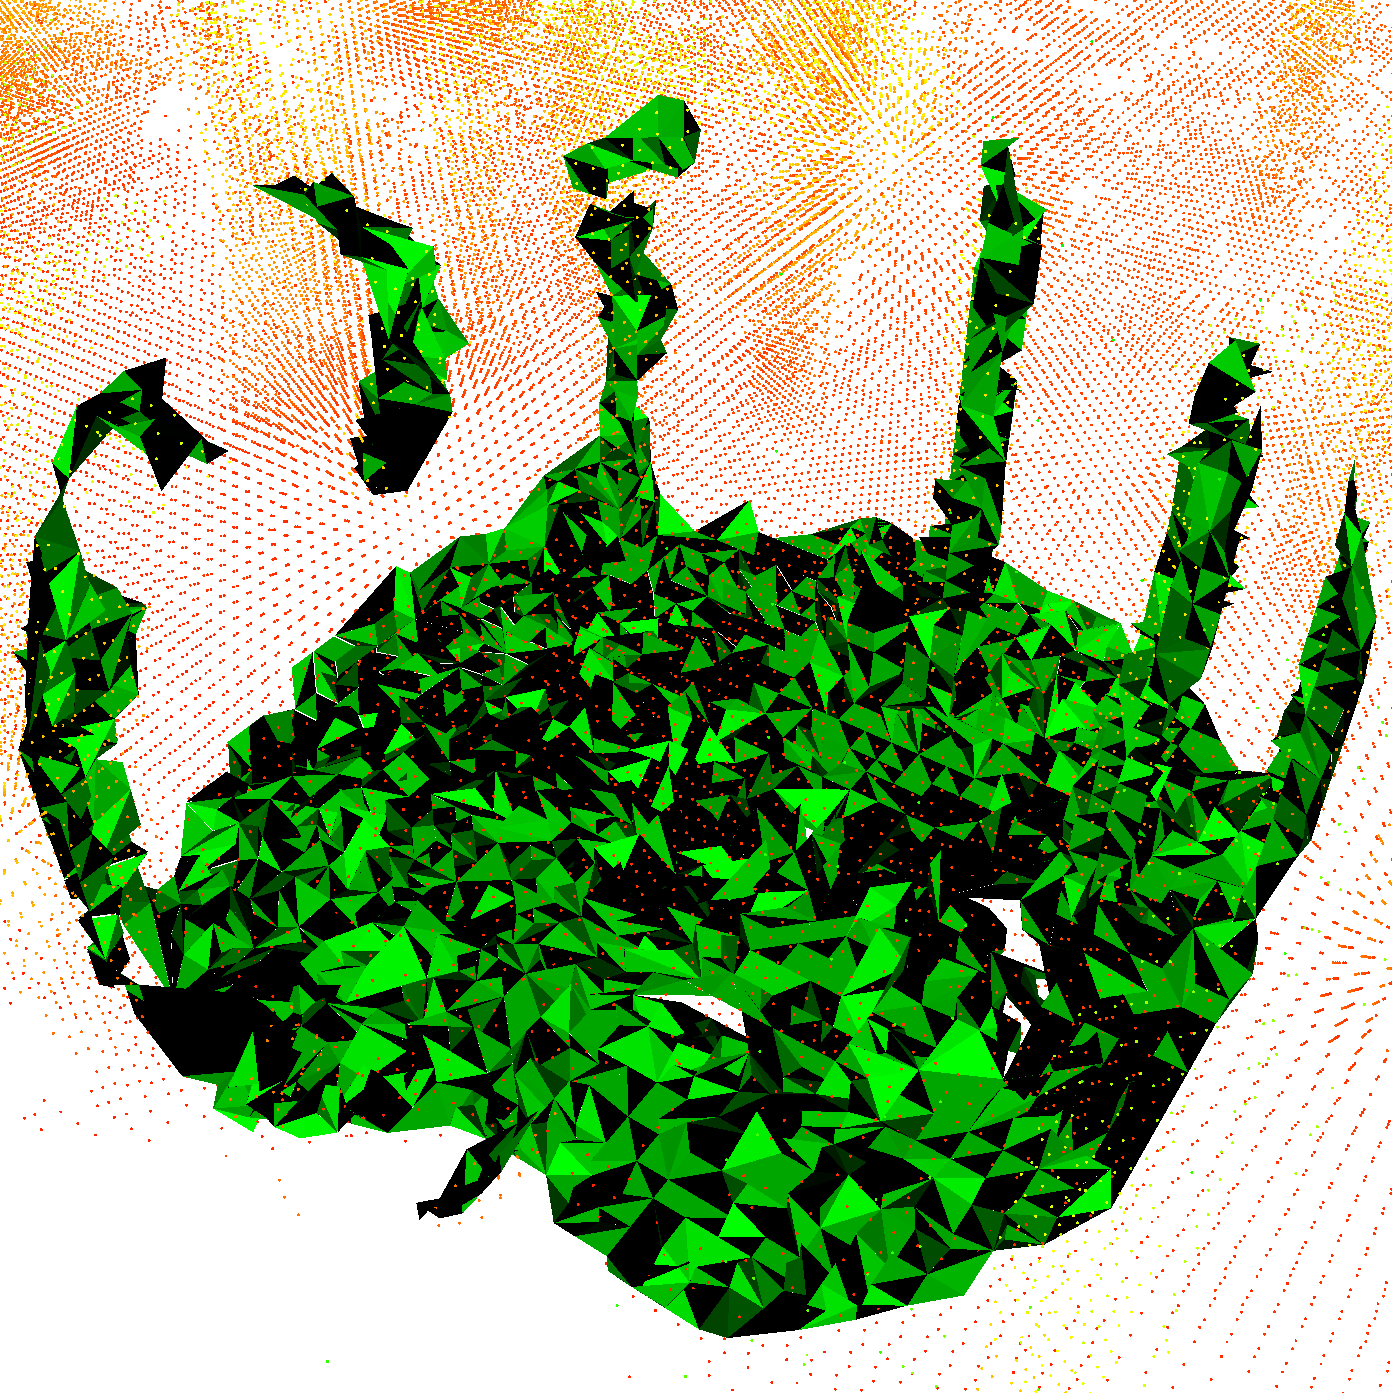
\includegraphics[width=0.48\textwidth]{./fig/rviz/triangulation_surface_aprox.png}
                \caption{
                    Surface approximation using Greedy Projection Triangulation.
                }
                \label{fig:triangulation}
            \end{figure}

        \subsection{Voxel-Based Modification of Cell $\mathcal{A}$}
            Given that the size of the voxels is known, this information can be used to refine the partitioning of cell $\mathcal{A}$ by treating voxels as obstacles.
            First, it is necessary to determine which voxels are relevant to the \ac{RBL} algorithm.
            This can be achieved by considering the scaling parameter $\eta$.
            A voxel is considered relevant if it lies within a radius of $\frac{r_s}{\eta}$ of the agent.
            For each discrete point in the cell $\mathcal{S}$, the nearest voxel is identified using a k-d tree algorithm from the \ac{PCL} library \cite{kd_tree}.
            Because the found point is the voxel's center, the closest point within that voxel's boundaries is calculated to accurately partition the cell $\mathcal{A}$ from cell $\mathcal{S}$.

            Given a point $\mathbf{p_{\mathcal{S}}}$, the voxel center $\mathbf{v_c}$ and the voxel edge length $\mathbf{e}$, $\mathbf{p}_{\text{closest}}$ is computed as: 
            \begin{equation}
                \mathbf{p}_{\text{closest}} =
                \begin{pmatrix}
                    \text{f}(p_{\mathcal{S},x}, v_{c,x} - \frac{\mathbf{e}}{2}, v_{c,x} + \frac{\mathbf{e}}{2}) \\
                    \text{f}(p_{\mathcal{S},y}, v_{c,y} - \frac{\mathbf{e}}{2}, v_{c,y} + \frac{\mathbf{e}}{2}) \\
                    \text{f}(p_{\mathcal{S},z}, v_{c,z} - \frac{\mathbf{e}}{2}, v_{c,z} + \frac{\mathbf{e}}{2})
                \end{pmatrix}\text{,}
            \end{equation}
            where the function f(x, a, b) constrains the value x to the range [a, b].
            This constrains $\mathbf{p_{\mathcal{S}}}$ to the voxel boundaries.
            
            Considering the point $\mathbf{p}_{\text{closest}}$ as an obstacle, the sensing cell $\mathcal{S}$ is partitioned to form cell $\mathcal{A}$ using the same procedure as \refeq{eqn:voronoi_cell_account_encum} (considering the closest point as another agent) encumbrance of the obstacle is not needed, because the closest point has been already found.
            The sensing cell $\mathcal{S}$ is partitioned to form the operational cell $\mathcal{A}$ by treating $\mathbf{p}_{\text{closest}}$ (the nearest point on an obstacle) as an agent and applying the procedure from Equation \eqref{eqn:voronoi_cell_account_encum}, the obstacle's full encumbrance is not required for this step because $\mathbf{p}_{\text{closest}} = \tilde{\mathbf{p}}_{j}$ provides the relevant point for partitioning $\mathcal{A}$, therefore $\delta_j = 0$.
            % This partition involves excluding any point $\mathbf{p_{\mathcal{S}}}$ from  $\mathcal{S}$ if its position relative to the agent $\mathbf{p}_i$ and the obstacle point $\mathbf{p}_{\text{closest}}$ meet condition $\mathcal{A}$ if $ \| \mathbf{p_i} - \mathbf{p_{\mathcal{S}}} \| \leq \eta \cdot \| \mathbf{p_i} - \mathbf{p}_{closest}\|$.

            % Using this point we can consider him as an obstacle and partition him out of sensing cell to form cell A. 
            % A point $\mathbf{p_{\mathcal{S}}}$ is excluded from the cell $\mathcal{A}$ if $ \| \mathbf{p_i} - \mathbf{p_{\mathcal{S}}} \| \leq \eta \cdot \| \mathbf{p_i} - \mathbf{p}_{closest}\|$.
            

    \section{Implementation and Integration on UAV}
    \label{sec:implementation_integration}
        \subsection{Challenges in Integration}
            The algorithm's performance is influenced by the limitations of the \ac{LiDAR} sensor used for environmental sensing. 
            While the algorithm works optimally with a full 360° horizontal and 180° vertical \ac{FOV}, which would require multiple sensors, the experiments used a single Livox Mid 360 \ac{LiDAR} \cite{livox_mid360}. 
            This \ac{LiDAR} provides a 360° horizontal \ac{FOV} and only a 59° vertical \ac{FOV}, resulting in a sensing blind spot.

            To solve this limitation, several modifications were implemented. 
            The \ac{LiDAR} was mounted at an angle $\gamma$, as shown in Figure \reffig{fig:uavs}, to enhance ground sensing and increase forward visibility.

            \begin{figure}[htbp]
                \centering
                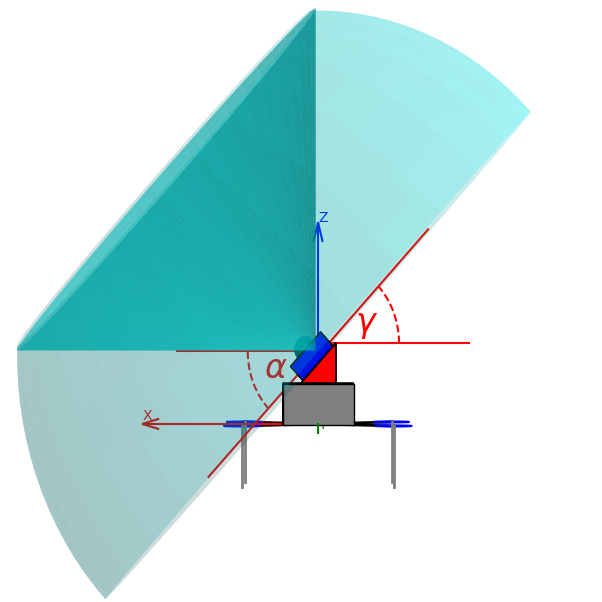
\includegraphics[width=0.48\textwidth]{./fig/photos/uav_side_view.png}
                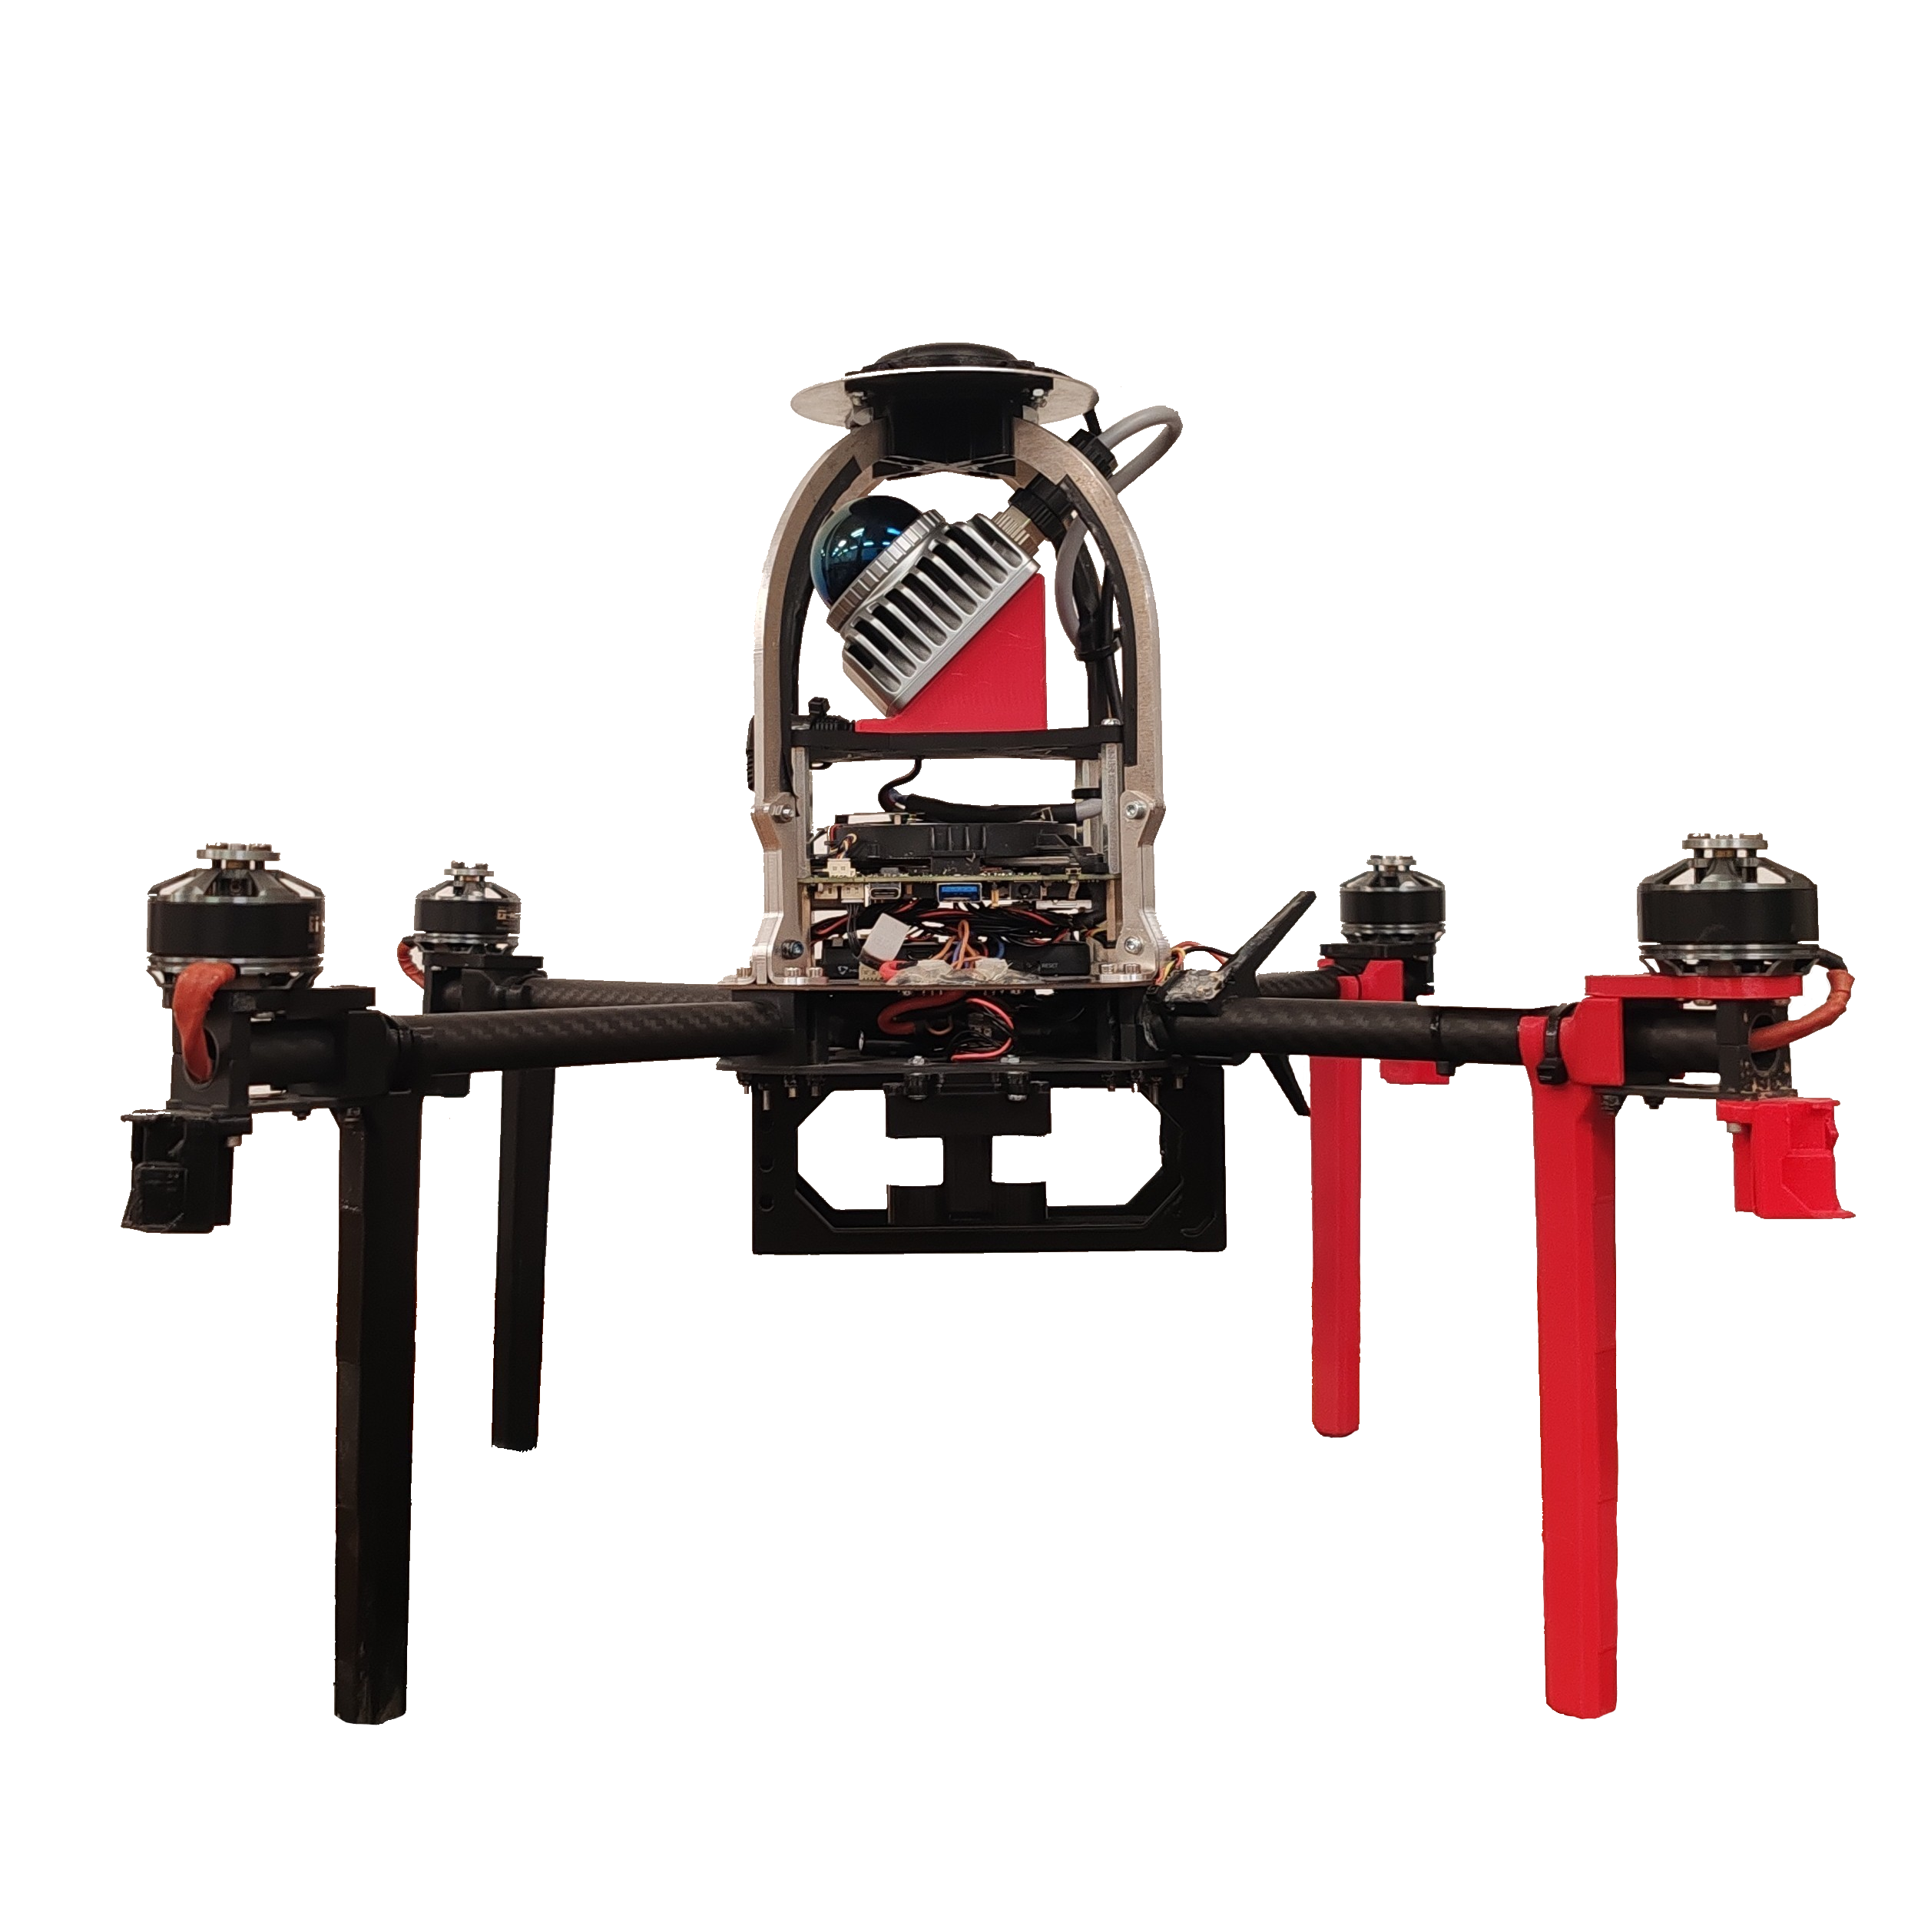
\includegraphics[width=0.48\textwidth]{./fig/photos/uav_photo.png}
                \caption{
                    \ac{UAV} and \ac{LiDAR} mounting scheme.
                    Please note that a different mounting angle was used in practical experiments, so the configuration shown here is purely for visualization purposes.
                    Subfigure on the left shows a modeled \ac{UAV} with visualized \ac{LiDAR} mounting parameters, including the \ac{LiDAR} elevation field of view $\alpha$ and tilt angle $\gamma$. 
                    Subfigure on the right displays the real \ac{UAV} used in the experiment with the \ac{LiDAR} mounted according to the same configuration.                                                
                }
                \label{fig:uavs}
            \end{figure}

            In addition to the \ac{LiDAR} mounting angle, a software modification is implemented to account for the \ac{LiDAR}'s limited \ac{FOV}.
            The algorithm uses the map to partition cell $\mathcal{S}$ into cell $\mathcal{A}$, from which the centroid is computed to guide \ac{UAV} movement.
            To ensure safety, the \ac{UAV} should only move within its visible \ac{FOV}. 
            However, the map information from areas outside the current \ac{FOV} can still be valuable. 

            Therefore, the following constraint is introduced - the \ac{UAV} maintains its yaw rotation towards the current centroid $\mathbf{c}_{\mathcal{A}}$ and moves towards the centroid only when the centroid is positioned within a $\pm \frac{\pi}{4}$ rad angular range from the direction the \ac{LiDAR} is tilted towards (the \ac{UAV}'s x-axis).
            This $\frac{\pi}{2}$ rad forward sector for movement is determined by the \ac{UAV}'s physical structure, specifically to prevent the \ac{UAV} from moving into areas where mounting rods for \ac{GPS} obstruct active sensing.

            To integrate the \ac{LiDAR}'s \ac{FOV} into cell $\mathcal{S}$, two planes are defined based on the \ac{LiDAR}'s mounting configuration and vertical \ac{FOV}.
            Let $\mathbf{e}_z$ be a unit vector along the z-axis, $R_{\gamma} \in SO(3)$ the tilt of the \ac{LiDAR}, and $R_{rpy} \in SO(3)$ the roll-pitch-yaw rotation.
            The normal vectors, $\mathbf{n}_1$ and $\mathbf{n}_2$ defining two planes are given by:
            \begin{equation}
                \mathbf{n}_1 = R_{rpy} R_{y}(\gamma)  \mathbf{e}_z    
            \end{equation}
            \begin{equation}
                \mathbf{n}_2 = R_{rpy} R_{y}(\gamma - \alpha) \mathbf{e}_z  \text{,}
            \end{equation}
            where $\alpha$ is the \ac{LiDAR}'s \ac{FOV} and $\gamma$ is the mounting angle of the \ac{LiDAR}, and $R_{rpy} = R_x(\text{roll})R_y(\text{pitch})R_z(\text{yaw})$.
            Cell $\mathcal{S}_i$ is then modified by excluding points that lie outside the \ac{LiDAR}'s \ac{FOV}, defined by these two planes: 

            \begin{equation}
                \mathcal{S}_i' = \{ \mathbf{q} \in \mathcal{S}_i \mid \mathbf{n}_1 \cdot (\mathbf{q} - \mathbf{p}_{L}) \geq 0 \land \mathbf{n}_2 \cdot (\mathbf{q} - \mathbf{p}_{L}) \leq 0 \}\text{,}
            \end{equation}
            where $\mathcal{S}_i'$ is the modified cell $\mathcal{S}_i$ and $\mathbf{p}_{L}$ is the exact position of the LiDAR sensor.

            This modification effectively restricts the points considered in the calculation of the centroid to only those within the \ac{LiDAR}'s \ac{FOV}.

            To integrate map information from the surrounding area outside of the \ac{LiDAR}'s current \ac{FOV}, the following procedure is used.
            Firstly, both cells $\mathcal{S}_i$ and $\mathcal{S}_i'$ are created. These cells are partitioned into cells $\mathcal{A}_i$ and $\mathcal{A}_i'$ using voxels. 
            Cell $\mathcal{A}_i'$ is partitioned using voxels that are actively sensed, while cell $\mathcal{A}_i$ is partitioned using the voxels from the whole surroundings.

            If the centroid computed from cell $\mathcal{A}_i$, $\mathbf{c}_{\mathcal{A}_i}$, is within the cell $\mathcal{A}_i'$, the \ac{UAV} is commanded to move towards $\mathbf{c}_{\mathcal{A}_i}$ while simultaneously rotating its yaw towards it.
            However, if $\mathbf{c}_{\mathcal{A}_i}$ lies outside cell $\mathcal{A}_i'$, it is projected onto the closest point on the boundary of cell $\mathcal{A}_i'$.
            As the \ac{UAV} only moves if the centroid is within a certain angle in front of it, this projection onto the boundary of $\mathcal{A}_i'$ ensures that the \ac{UAV} primarily rotates towards the centroid until the centroid is within an angle in front of the \ac{UAV}.
            This control logic is formally defined as follows:
            \begin{equation}
                \begin{cases}
                    \text{move and rotate towards } \mathbf{c}_{\mathcal{A}_i} & \text{if } \mathbf{c}_{\mathcal{A}_i} \in \mathcal{A}_i' \land \alpha \in [-\frac{\pi}{4}, \frac{\pi}{4}] \\
                    \text{only rotate, do not move towards } \mathbf{c}_{\mathcal{A}_i} & \text{otherwise, }
                \end{cases}
            \end{equation}
            where $\alpha = \text{atan2}((\mathbf{c}_{\mathcal{A}_i} - \mathbf{p}_i)_y, (\mathbf{c}_{\mathcal{A}_i} - \mathbf{p}_i)_x) - \text{yaw}_i$

            This procedure effectively utilizes the information from the map while ensuring that the \ac{UAV} moves only within its actively sensed \ac{FOV}.

            \begin{figure}[H]
                \centering
                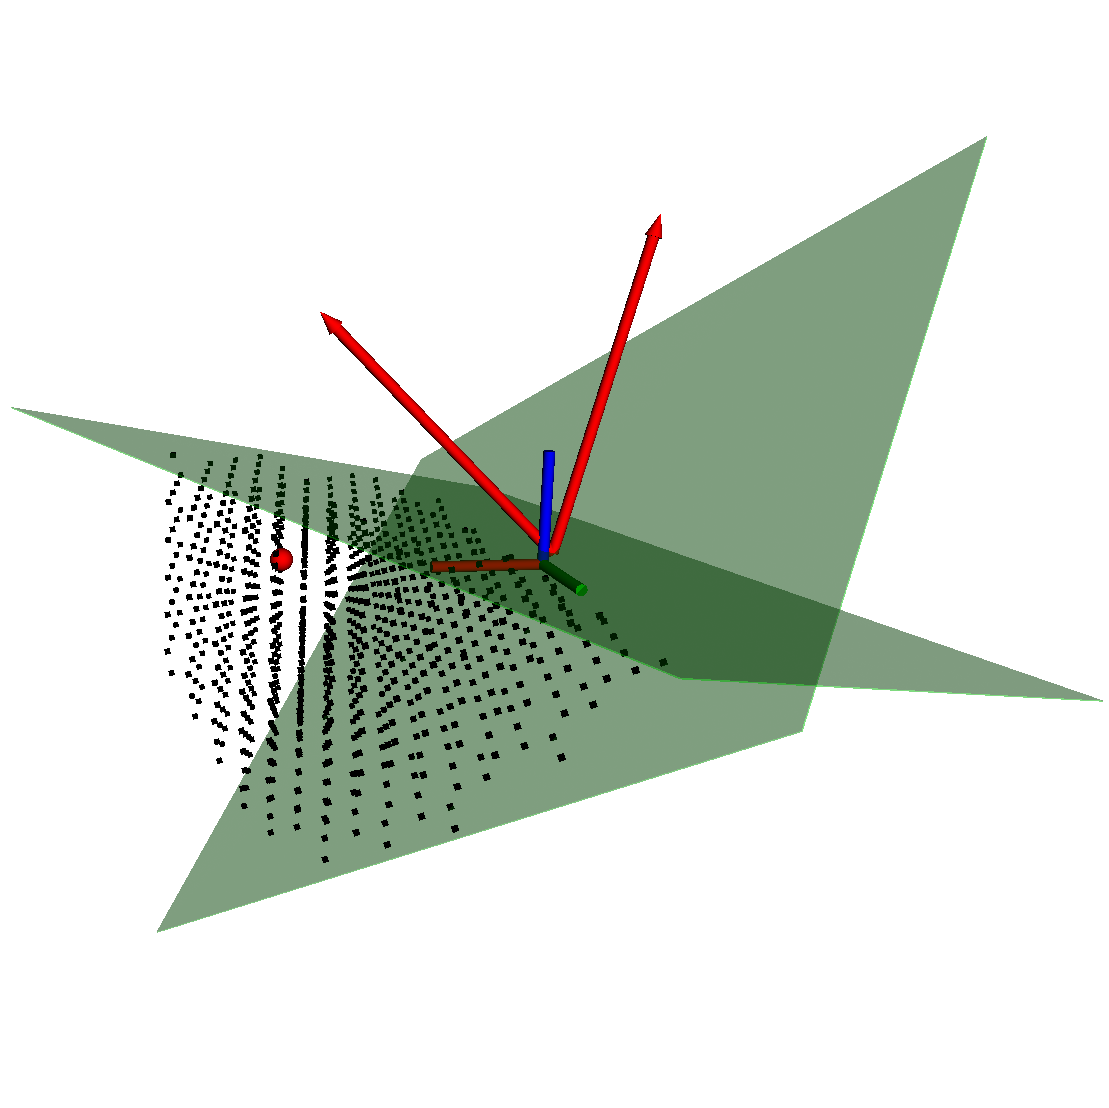
\includegraphics[width=0.48\textwidth]{./fig/rviz/cell_a_sliced_with_planes.png}
                \caption{
                    Rviz visualization of \ac{LiDAR} \ac{FOV} planes. The \ac{UAV} is represented by the XYZ coordinate axes. 
                    The green squares represent the two planes, defined by normal vectors $\mathbf{n}_1$ and $\mathbf{n}_2$, used to slice cell $\mathcal{S}_i$ and determine the modified cell $\mathcal{S}_i'$.
                    The red sphere represents the centroid $\mathbf{c}_{\mathcal{A}_i}$.
                }
                \label{fig:cell_a_sliced}
            \end{figure}
    
    \section{Experimental Results}
    \label{sec:experimental_results}
        This section presents the findings from both simulated and real-world experiments conducted to evaluate the proposed approach.
        \subsection{Simulation Setup}
            In the simulations, a virtual forest environment was created. 
            Initially, a raycasting approach from the \ac{UAV} to the simulated trees was considered for obstacle detection. 
            However, due to its computational cost, a static point cloud representation of the entire forest was generated and published instead. 
            The forest was modeled as a collection of trees, with trunks represented by cylinders and crowns by spheres.
            The forest was generated within a rectangular area defined by the opposing corner points (-20.0 m, -32.0 m) and (20.0 m, 32.0 m) in the x-y plane, with its sides aligned parallel to the x and y axes.
            % The forest was contained within a rectangular area defined by the following boundaries:
            % \begin{itemize}
            %     \item $x_{\min}$ = -20.0 m
            %     \item $x_{\max}$ =  20.0 m
            %     \item $y_{\min}$ = -32.0 m
            %     \item $y_{\max}$ =  32.0 m
            % \end{itemize}
            A total of 100 trees were randomly generated within this area, with a minimum separation distance of 3 meters between them. 
            The trees were generated with the following parameter variances:
            \begin{itemize}
                \item Trunk radius: 0.5 $\pm$ 0.2 m
                \item Tree height: 7.5 $\pm$ 2.0 m
                \item Crown radius: 2.5 $\pm$ 0.5 m
            \end{itemize}
            The \ac{UAV}'s starting position was set at one corner of the rectangular area (-22.0, -33.0, 2.0), and the goal position was set at the opposite corner (22.0, 33.0, 5.0).

            Note that the right-hand rule and z rule, described in the previous chapter, are not required for effective coordination in this static forest environment.
            Also, the \ac{Point-LIO} estimator and Bonxai mapping were not simulated.

            A separate simulation was also run to compare the 2D \ac{RBL} algorithm with its 3D extension, using a circle crossing setup in the forest.

            The specific values of the parameters used in the experiments are summarized in the following table \ref{tab:rbl_forest_simulation_parameters}:

            % \begin{table}[H]
            %     \centering
            %     \caption{Parameters Used in Experiments}
            %     \begin{tabular}{|l|l|l|l|l|l|l|l|}
            %         \hline
            %         % Row 1: Parameter names act as column headers here
            %         Parameter & $r_s$ [m]                  & Update rate [Hz] & $\delta_i$ [m]  & $d_1 = d_3 = d_5$  [m] & $d_2 = d_4 = d_6$ [m] & $\beta_i^D$ [] & $\eta$ []\\
            %         \hline \hline 
            %         Value     & 3.5                        & 10               & 0.5             & 0.5                    & 1.0                   & 0.5            & 0.9  \\
            %         \hline
            %     \end{tabular}
            %     \label{tab:rbl_forest_simulation_parameters_transposed} % Adjusted label
            % \end{table}

            % \begin{table}[H]
            %     \centering
            %     \caption{Parameters Used in Experiments}
            %     \begin{tabular}{|l|c|}
            %         \hline
            %         Parameter & Value \\
            %         \hline
            %         \hline
            %         Sensing radius $r_s$ [m] & 3.5 \\ \hline
            %         Update rate [Hz] & 10  \\ \hline
            %         Encumbrance $\delta_i$ [m] & 0.5  \\ \hline
            %         $d_1 = d_3 = d_5$ [m] & 0.5  \\ \hline
            %         $d_2 = d_4 = d_6$ [m] & 1.0  \\ \hline
            %         $\beta_i^D$ [ ] & 0.5  \\ \hline
            %         $\eta$ [ ] & 0.9  \\ \hline
            %     \end{tabular}
            %     \label{tab:rbl_forest_simulation_parameters}
            % \end{table}

            \begin{table}[H]
                \centering
                \caption{Parameters Used in Experiments}
                
                \begin{tabular}{|c|c|c|c|c|}
                    \hline
                    Parameter & $r_s$ [m]  & $\delta_i$ [m] & $d_1 = d_3 = d_5$ [m] & $d_2 = d_4 = d_6$ [m]   \\ \hline
                    Value & 3.5 & 0.5 & 0.5 & 1.0 \\ \hline
                \end{tabular}
                
                \vspace{0.3cm}
                
                \begin{tabular}{|c|c|c|c|c|}
                    \hline
                    Parameter & Update rate [Hz] & $\gamma$ [°] & $\beta_i^D$ [ ] & $\eta$ [ ] \\ \hline
                    Value & 10.0 & 20.0 & 0.5 & 0.9 \\ \hline
                \end{tabular}
                
                \label{tab:rbl_forest_simulation_parameters}
            \end{table}
            
            The \ac{UAV} dynamics are the same as described in the previous chapter and detailed in Table \ref{tab:uav_constraints}. 
            Each simulation was run 10 times with the same forest. 

        \subsection{Performance in Simulated Environments}
            The first simulation results highlight the proposed solution capability in navigating inside dense forest environments. 
            The \ac{UAV} demonstrated effective obstacle avoidance, reacting appropriately to simulated trees while maintaining an efficient trajectory without unnecessary detours.
            Convergence towards the designated goal was consistently achieved in a stable manner.

            \begin{table}[H]
                \centering
                \renewcommand{\arraystretch}{1.2}
                \begin{tabular}{|c|c|c|c|c|}
                \hline
                                                  & \( SR \ [\%] \) & \( \overline{L} \ [\mathrm{m}] \) & \( \overline{t} \ [\mathrm{s}] \) &  \( \overline{v} \ [\mathrm{m/s}] \)     \\ \hline
                Results                           & 100.00          & 91.99 $\pm$ 0.96                  & 150.89 $\pm$ 0.88                  &  0.85 $\pm$ 0.00                         \\ \hline
                \end{tabular}
            \end{table}

            \begin{figure}[H]
                \centering
                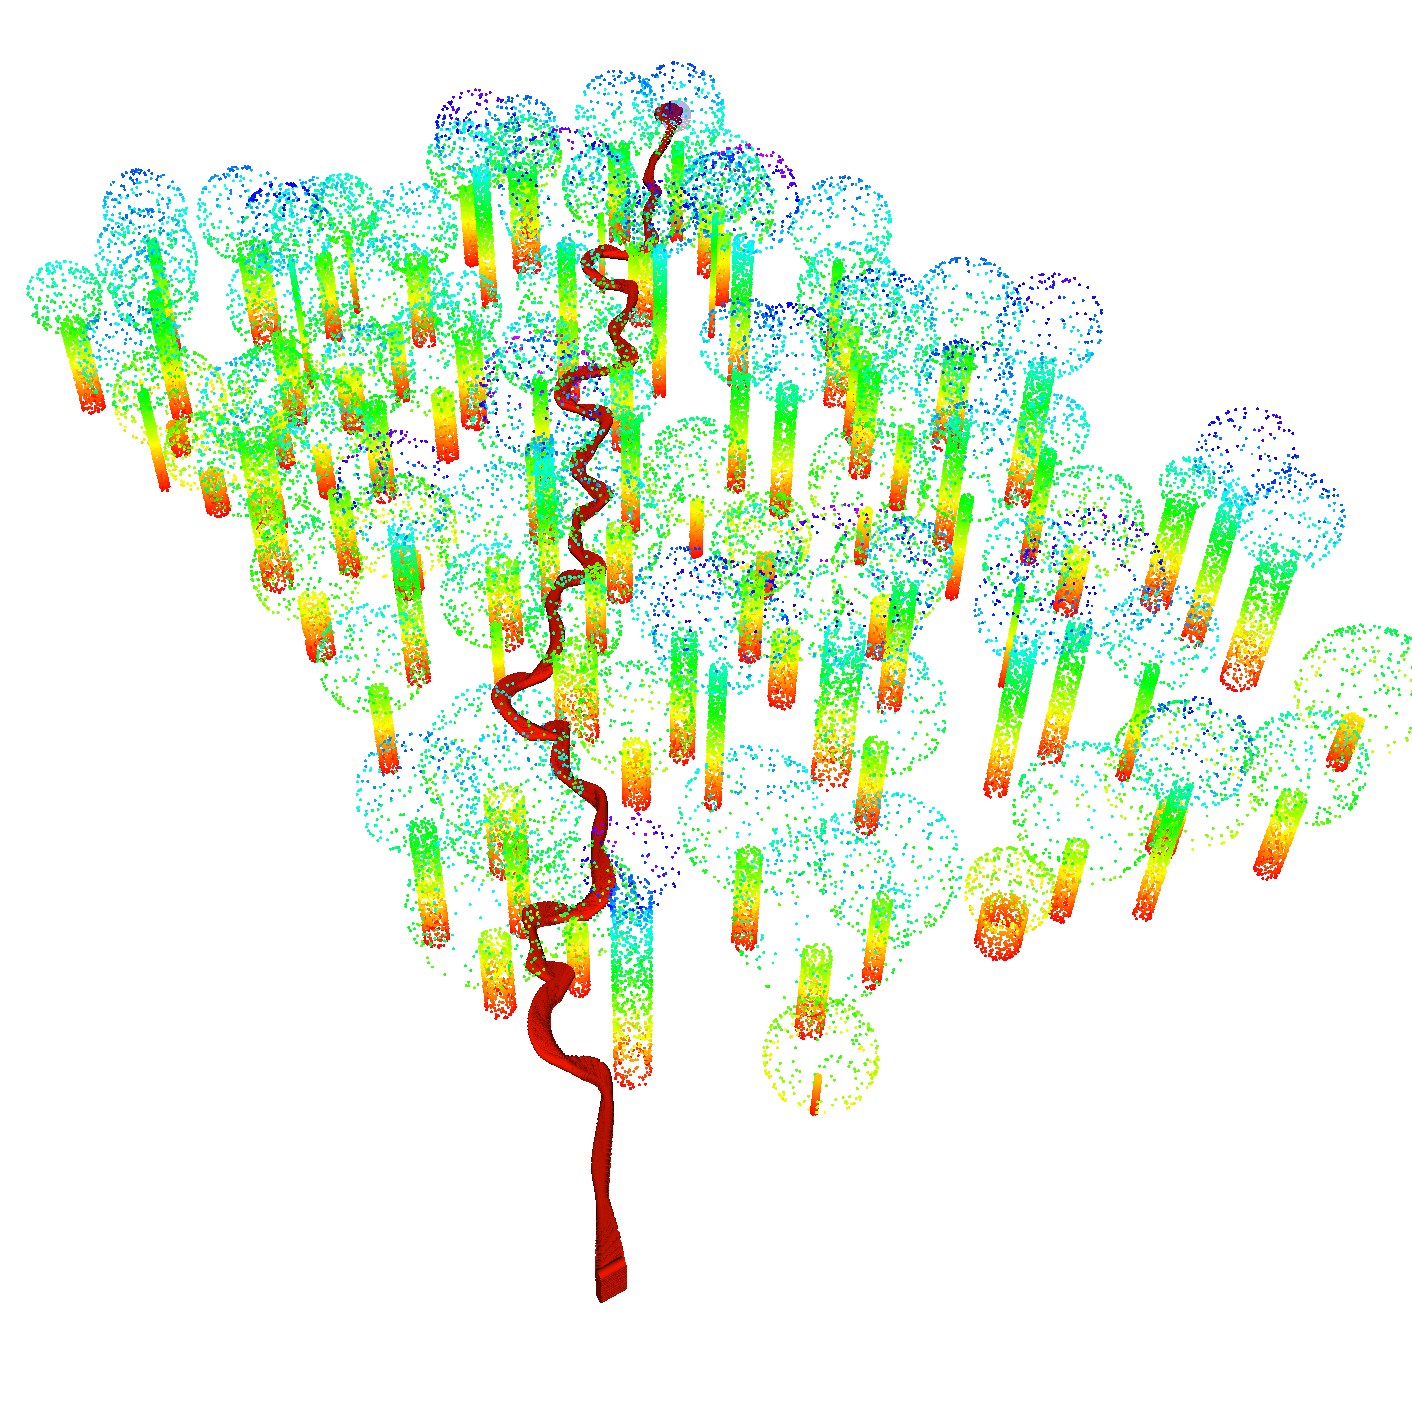
\includegraphics[width=0.48\textwidth]{./fig/rviz/simulation_forest.png}
                \caption{
                    Visualization of simulated forest and the corresponding path of the \ac{UAV}, indicated by a red line.
                }
                \label{fig:simulated_forest_path}
            \end{figure}

            Additional simulations directly compared the 2D and extended 3D \ac{RBL} algorithms in the static forest. 
            These results confirmed that \ac{UAV}s using the 3D \ac{RBL} were capable of consistently reaching the goal by exploring vertical dimensions, navigating above or below tree crowns. 
            The 2D \ac{RBL}, on the other hand, failed by getting stuck between the obstacles.
            \begin{table}[H]
                \centering
                \renewcommand{\arraystretch}{1.2}
                \begin{tabular}{|c|c|c|c|c|c|}
                \hline
                                                    & \( SR \ [\%] \)   & \( \overline{L} \ [\mathrm{m}] \)                & \( \overline{t} \ [\mathrm{s}] \)                & \( \overline{t}_{\text{max}} \ [\mathrm{s}] \)    &   \( \overline{v} \ [\mathrm{m/s}] \)     \\ \hline
                \ac{RBL} 2D                         & 0.00              & 30.27 $\pm$ 0.12                                 & $\infty$                                         &  $\infty$                                         &  0.00 $\pm$ 0.00                         \\ \hline
                \ac{RBL} $\text{3D}_{\text{rule}}$  & $\mathbf{100.00}$ & $\mathbf{28.40} \boldsymbol{\pm} \mathbf{10.68}$ & $\mathbf{50.90} \boldsymbol{\pm} \mathbf{33.51}$ &  $\mathbf{99.86} \boldsymbol{\pm} \mathbf{16.01}$ &  $\mathbf{0.54} \boldsymbol{\pm} \mathbf{0.27}$                         \\ \hline
                \end{tabular}
            \end{table}

            \begin{figure}[htbp]
                \centering
                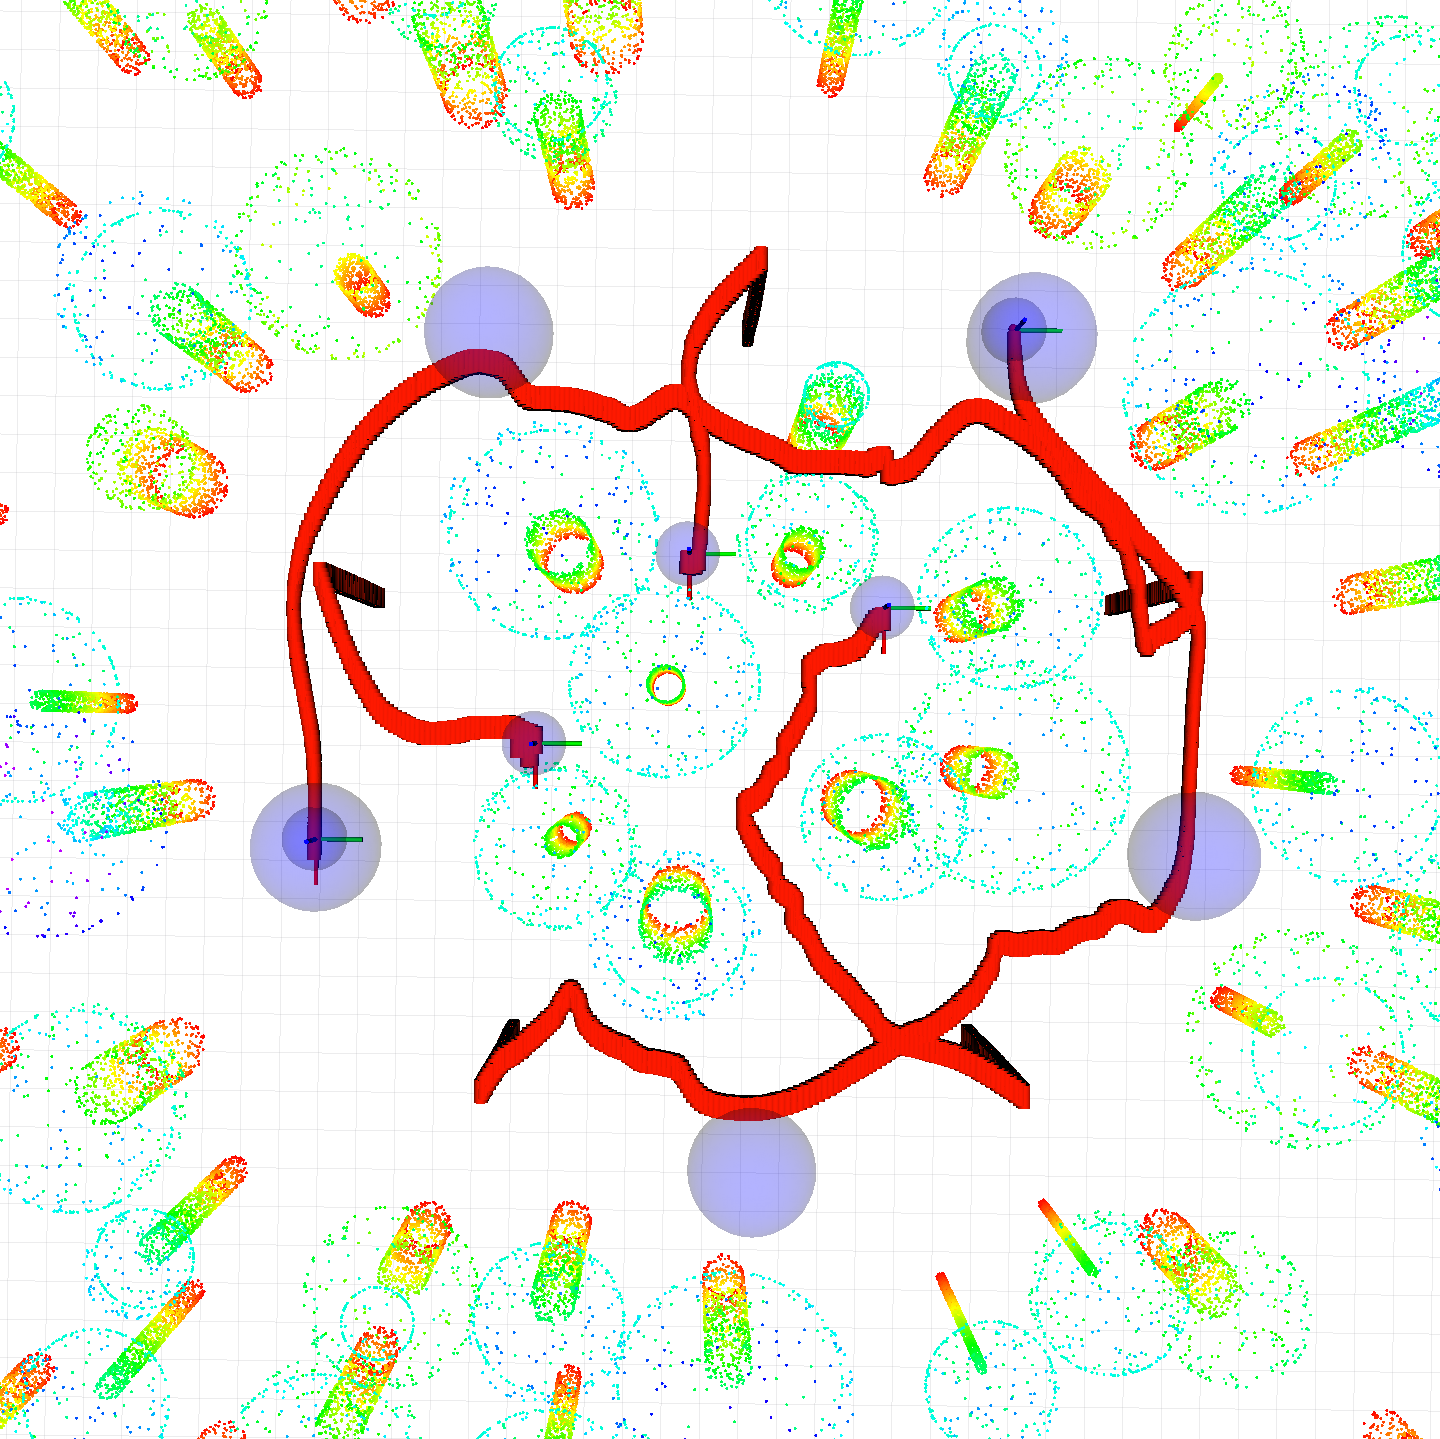
\includegraphics[width=0.48\textwidth]{./fig/rviz/circular_forest_fail.png}
                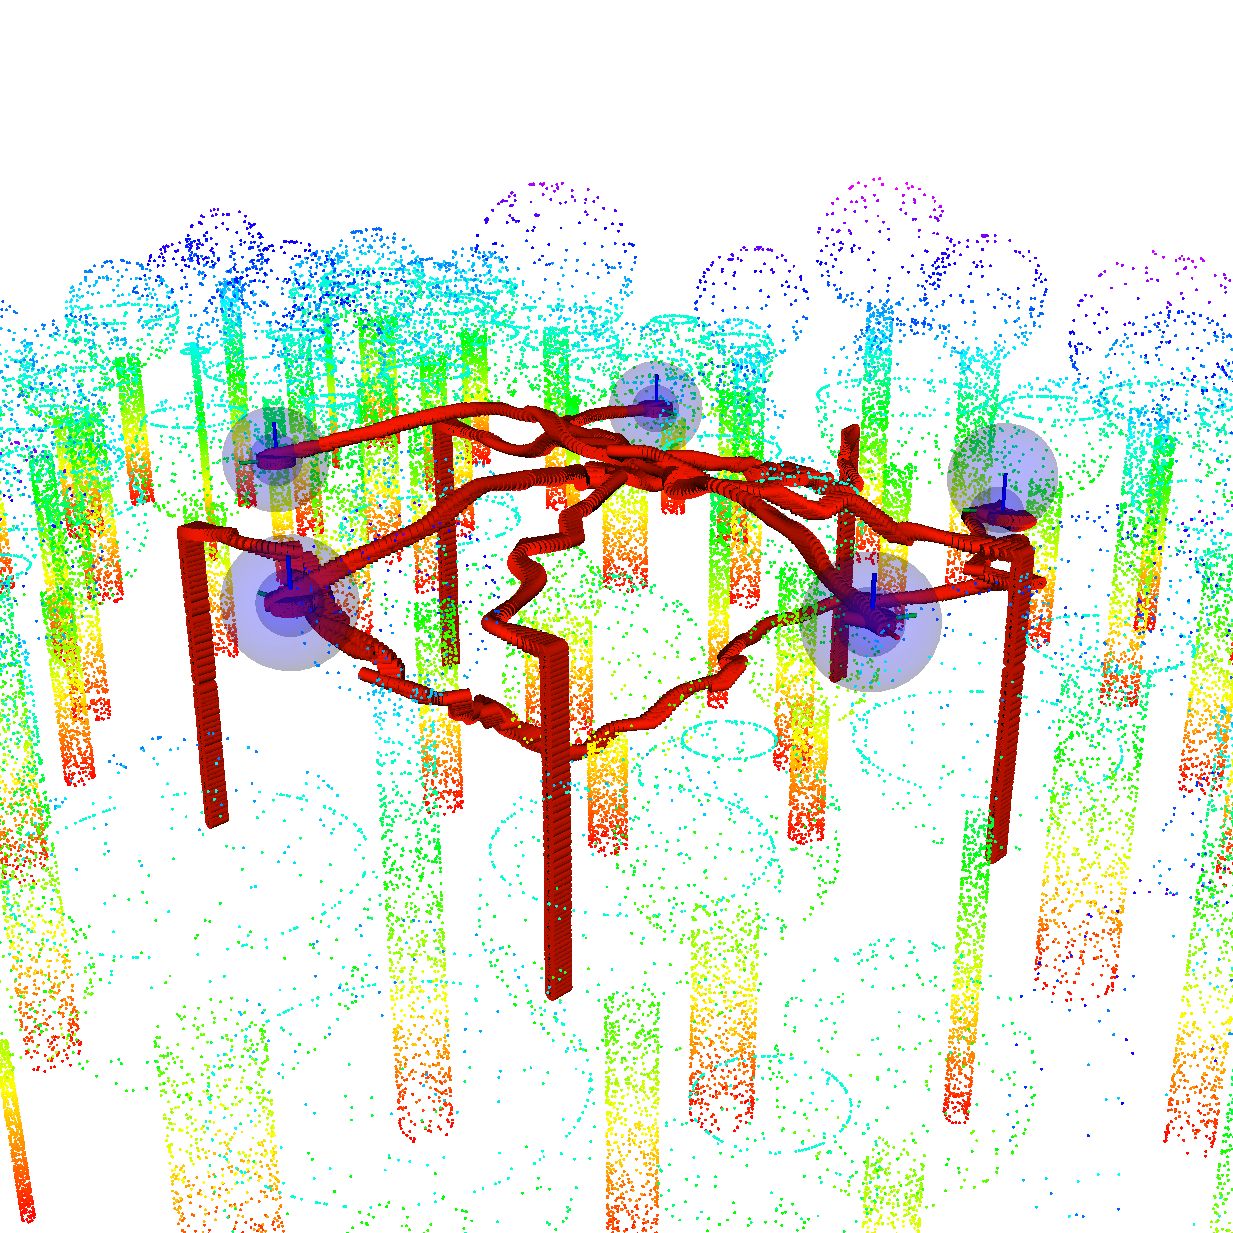
\includegraphics[width=0.48\textwidth]{./fig/rviz/3d_crossing_circle_forest.png}
                \caption{
                    Illustrative comparison of 2D and 3D RBL navigation capabilities in a simulated forest environment. 
                    Left: The 2D algorithm is shown in a deadlock. 
                    Right: The 3D algorithm demonstrates its ability to utilize vertical space.
                }
                \label{fig:forest_crossing_circle}
            \end{figure}

        \subsection{Real-World Experiments in a Forest Environment}
            Following the successful simulation validation, the \ac{RBL} algorithm was tested through real-world experiments conducted in a forest environment.
            \begin{itemize}
                \item \textbf{Location: } \\
                    The forest site for initial real-world experiments was chosen for its relatively open characteristics, allowing for straightforward system validation. 
                    Subsequent flight tests were then conducted in more challenging and densely obstructed environments.
                    To increase the navigational challenge and better test the obstacle avoidance capabilities, additional branches were placed near trees within the flight area after a few successful flights. 
                    % The point cloud filtration parameters were set to discard points closer than 1.0 meter (to avoid detecting the \ac{UAV}'s own propellers) and farther than 40 meters.
                \item \textbf{UAV Platform: } \\
                    % A custom-built multirotor \ac{UAV} from the MRS group was used for this experiment X500. 
                    A custom-built multirotor \ac{UAV} from the \ac{MRS} group, the X500, was used for these experiments.
                    It was equipped with \ac{LiDAR} mounted on top for environmental perception and state estimation.
                    While other sensors like \ac{GPS} (unreliable in the forest), a Garmin altimeter, and barometer were present on the platform, they were not used.
                % \item \textbf{Experimental Procedure: } \\
                %     Each experimental run followed a defined procedure. 
                %     First, the necessary software components were launched within a tmux session on the ground. 
                %     A safety pilot then armed the \ac{UAV} and performed a manual takeoff to a safe altitude. 
                %     Once airborne and stable, the \ac{RBL} algorithm was initiated, commanding the \ac{UAV} towards a predefined goal. 
                %     The flight was continuously monitored via visualization in Rviz and observing the \ac{UAV}. 
                %     If the \ac{UAV} approached an obstacle too closely or exhibited unsafe behavior, the safety pilot immediately terminated the autonomous mode, took manual control, and landed the \ac{UAV}. 
                %     Between runs, key algorithm parameters, such as those controlling navigation 'aggressivity' (e.g., the scale of cells in the RBL and the weighting function used for path planning), were adjusted based on observations from the previous flight, and the experiment was repeated.
                % \item \textbf{Safety Measures: } \\
                %     Safety was paramount throughout the experiments. 
                %     A trained safety pilot maintained visual line-of-sight with the \ac{UAV} at all times and was prepared to immediately take manual control via the remote controller should any unsafe condition arise.
                % \item \textbf{Data Collected: } \\
                %     For safety reasons, data logging was initiated only after the manual takeoff was complete. 
                %     During the autonomous flight part and subsequent landing, all relevant ROS topics (including sensor data, estimated state, \ac{RBL} cells, centroid) were recorded into rosbag files for detailed post-flight analysis.
                % \item \textbf{Challenges Encountered: } \\
                %     Several challenges emerged during real-world deployment. 
                %     A significant set-back involved correctly managing coordinate frame transformations, particularly due to the slight tilt of the top-mounted LiDAR sensor. 
                %     Ensuring accurate alignment between the LiDAR's point cloud data, the \ac{Point-LIO} state estimator, and the navigation algorithm's reference frame required careful configuration. 
                %     Another challenge, which warrants further investigation (discussed in Future Work), related to the Bonxai mapping part. 
                %     Occasionally, the mapper would map dynamic objects, such as leaves disturbed by propellers, into the static map. 
                %     Due to the mapping algorithm's configuration, which was set to be conservative about removing potentially static obstacles to ensure safety, these incorrectly mapped 'ghost' obstacles were sometimes not removed even when subsequent scans showed they were no longer present. 
                %     In some instances, this led to the \ac{UAV} perceiving itself as surrounded by obstacles (effectively 'locking' itself), requiring the safety pilot to intervene and land.
            \end{itemize}

            \begin{figure}[htbp]
                \centering
                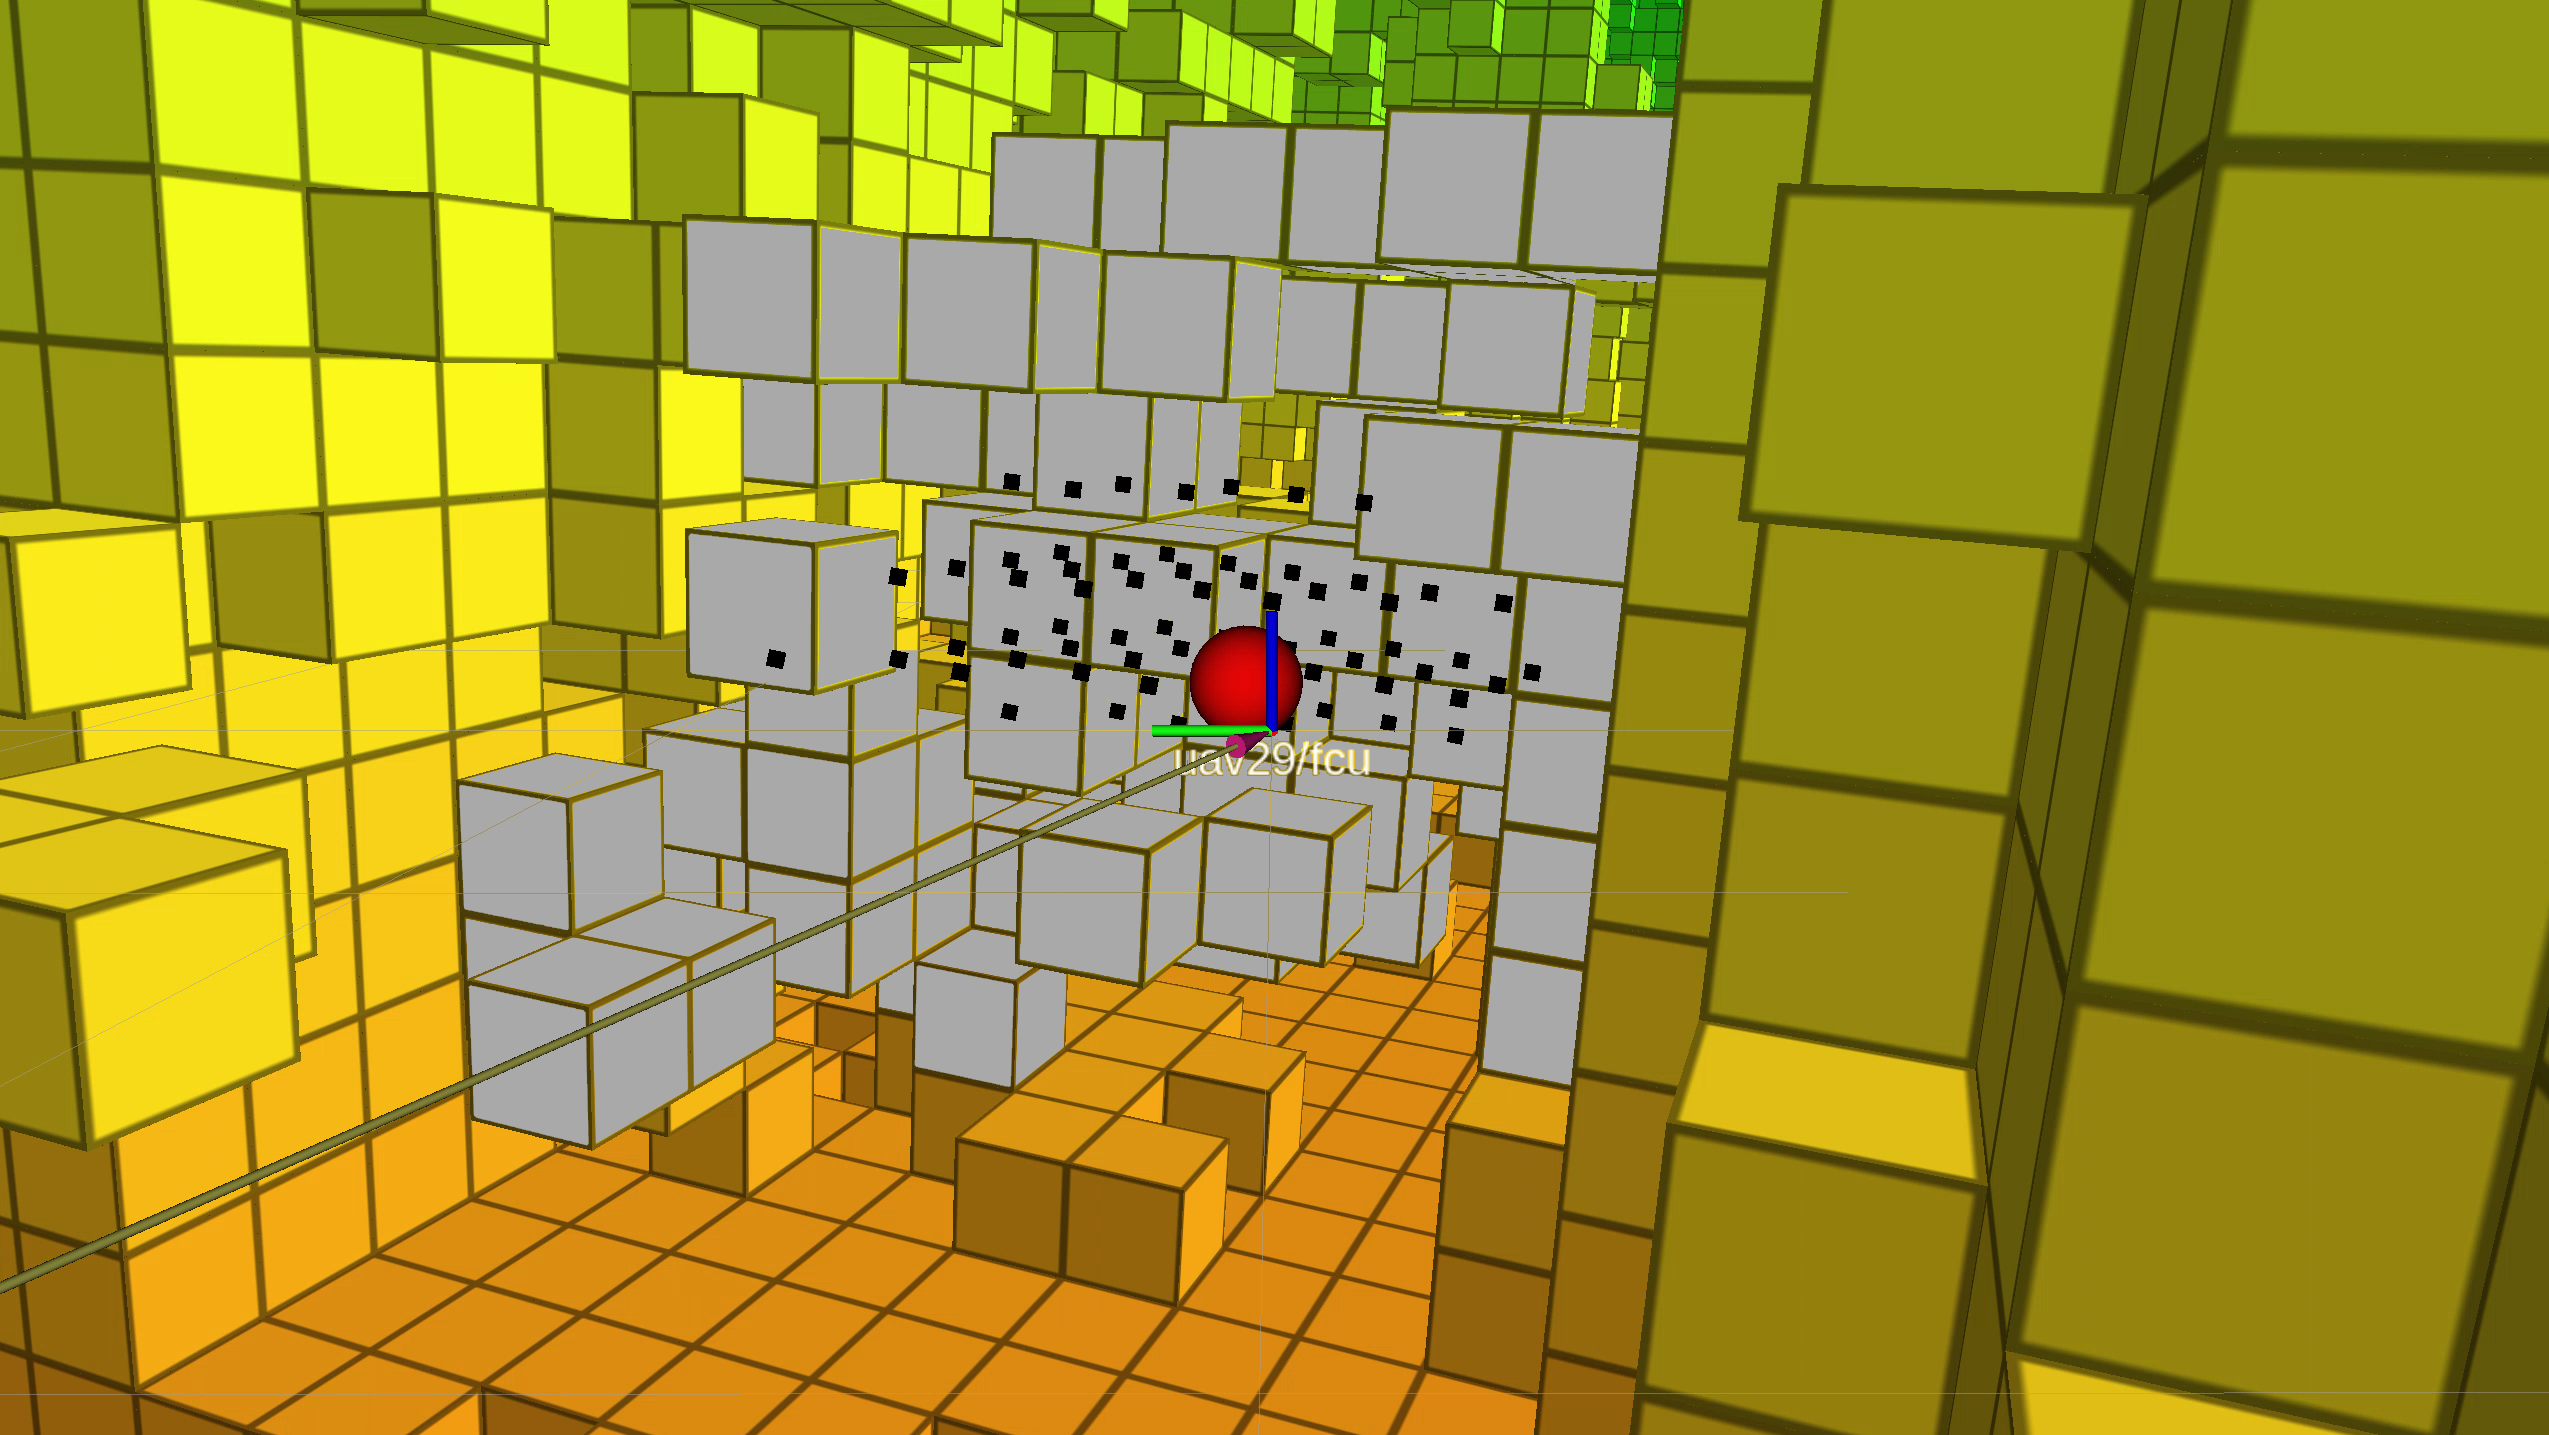
\includegraphics[width=0.96\textwidth]{./fig/rviz/deadlock_moment_mapping_gray.png}
                \caption{
                    Visualization of a moment where the \ac{UAV} incorrectly mapped leaves as obstacles directly in its path. 
                }
                \label{fig:map_fail}
            \end{figure}

        
        \subsection{Performance in Real-World Experiment}
            For the real-world experiment I picked 2 flights to describe and one fail flight. 
            For these flights the point cloud filtration parameters were set to discard points closer than 1.0 meter (to avoid detecting the \ac{UAV}'s own propellers) and farther than 40 meters.
            For both flights a video has been created to show the performance \href{https://www.youtube.com/watch?v=DFt222gnA_w&ab_channel=MichalKamler}{aggressive flight} \cite{aggressive_flight}, \href{https://www.youtube.com/watch?v=AJPk0yVCPUo&ab_channel=MichalKamler}{conservative flight}\cite{conservative_flight}.
            
            \begin{figure}[htbp]
                \centering
                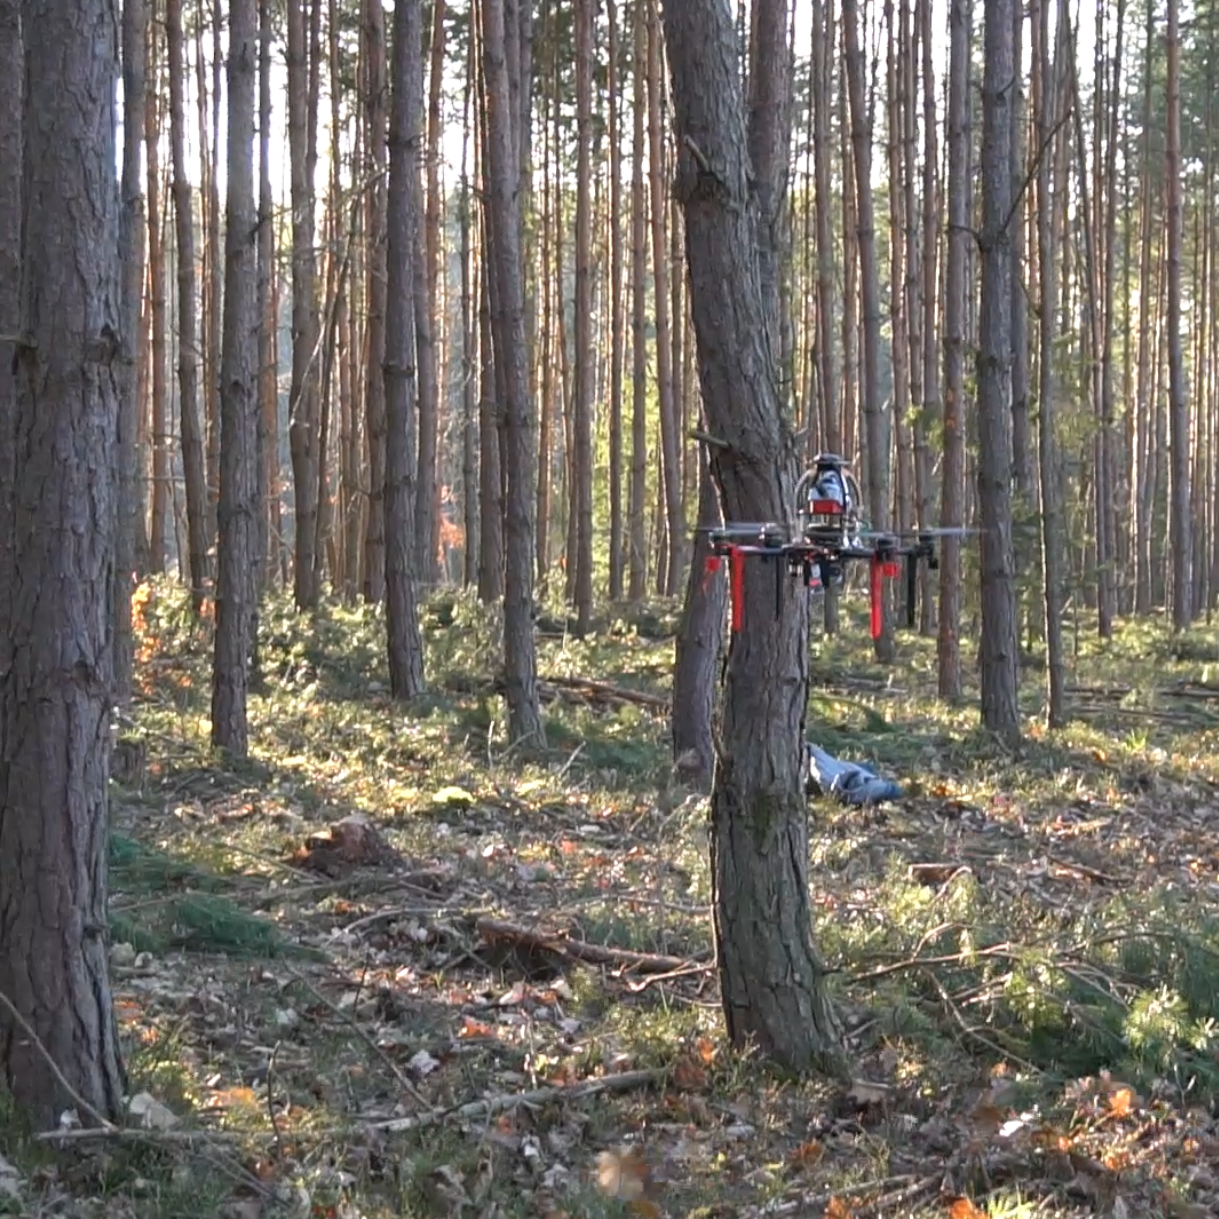
\includegraphics[width=0.48\textwidth]{./fig/photos/pic1.png}
                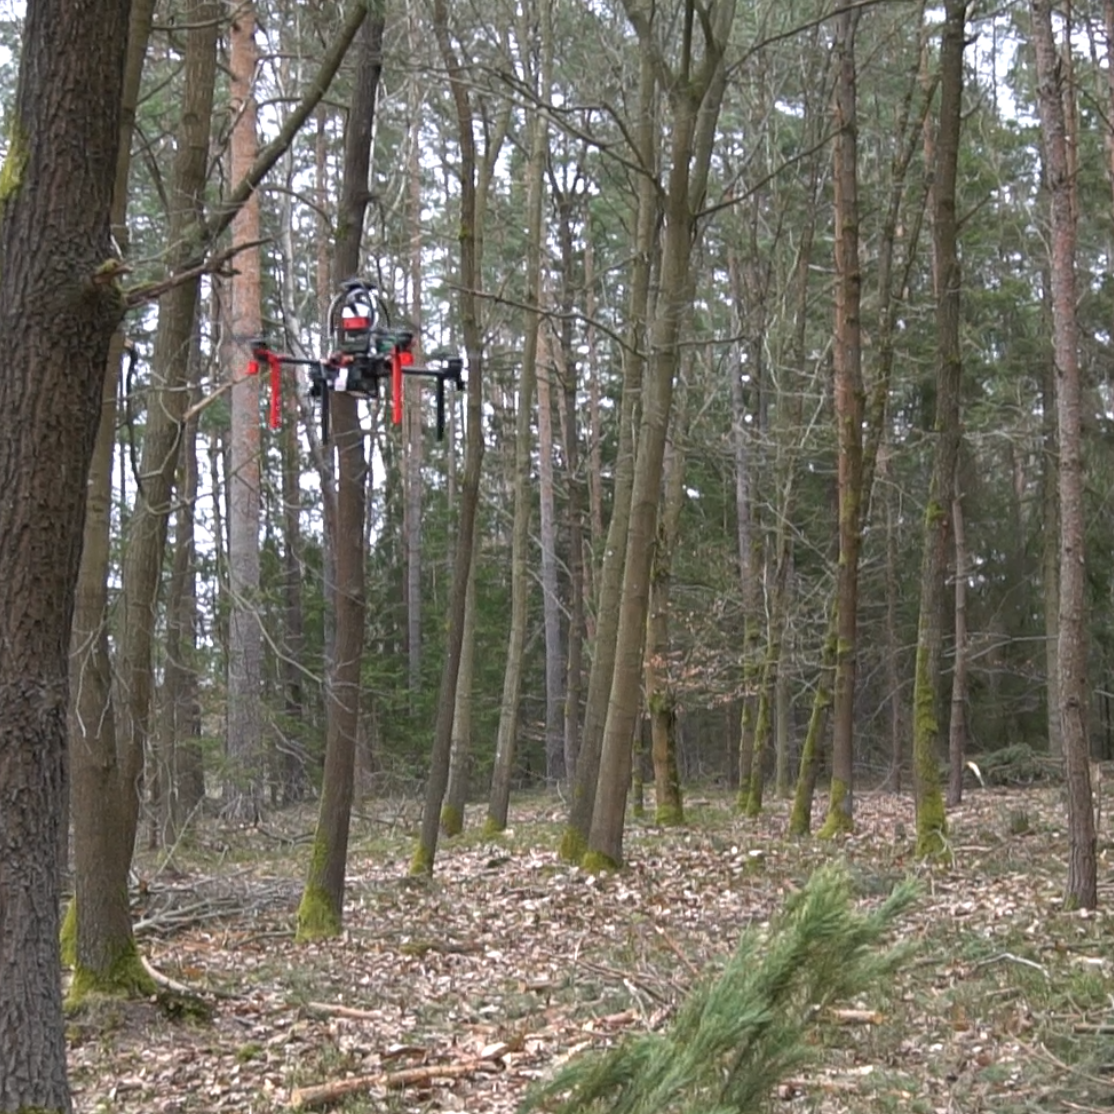
\includegraphics[width=0.48\textwidth]{./fig/photos/pic2.png}
                \caption{
                    The \ac{UAV} navigating in a forest during an experiment. 
                }
                \label{fig:real_wrld_pics}
            \end{figure}

            \begin{table}[H]
                \centering
                \caption{Parameters Used in Experiments}
                \begin{tabular}{|c|c|c|}
                    \hline
                    Parameter & Values Conservative & Values Aggressive \\
                    \hline
                    $r_s$ [m] & 2.0 & 2.0 \\ \hline
                    Update rate [Hz] & 10 & 10 \\ \hline
                    $\delta_i$ [m] & 0.5 & 0.5  \\ \hline
                    $d_1 = d_3 = d_5$ [m] & 0.5 & 0.5  \\ \hline
                    $d_2 = d_4 = d_6$ [m] & 1.0 & 1.0 \\ \hline
                    $\gamma$ [°] & 20.0 & 20.0 \\ \hline
                    $\beta_i^D$ [ ] & 0.5 & 0.1 \\ \hline
                    $\eta$ [ ] & 0.8 & 0.8 \\ \hline
                \end{tabular}
                \label{tab:rbl_forest_conservative_flight}
            \end{table}

            \begin{table}[H]
                \centering
                \renewcommand{\arraystretch}{1.2}
                \begin{tabular}{|c|c|c|c|c|}
                \hline
                                    & \( L \ [\mathrm{m}] \) & \( t \ [\mathrm{s}] \) &  \( v \ [\mathrm{m/s}] \)     \\ \hline
                Conservative Flight & 53.84                   & 116.40                  &  0.46                          \\ \hline
                Aggressive Flight    & 35.56                   &  51.64                  &  0.69                          \\ \hline
                \end{tabular}
            \end{table}

            \begin{figure}[htbp]
                \centering
                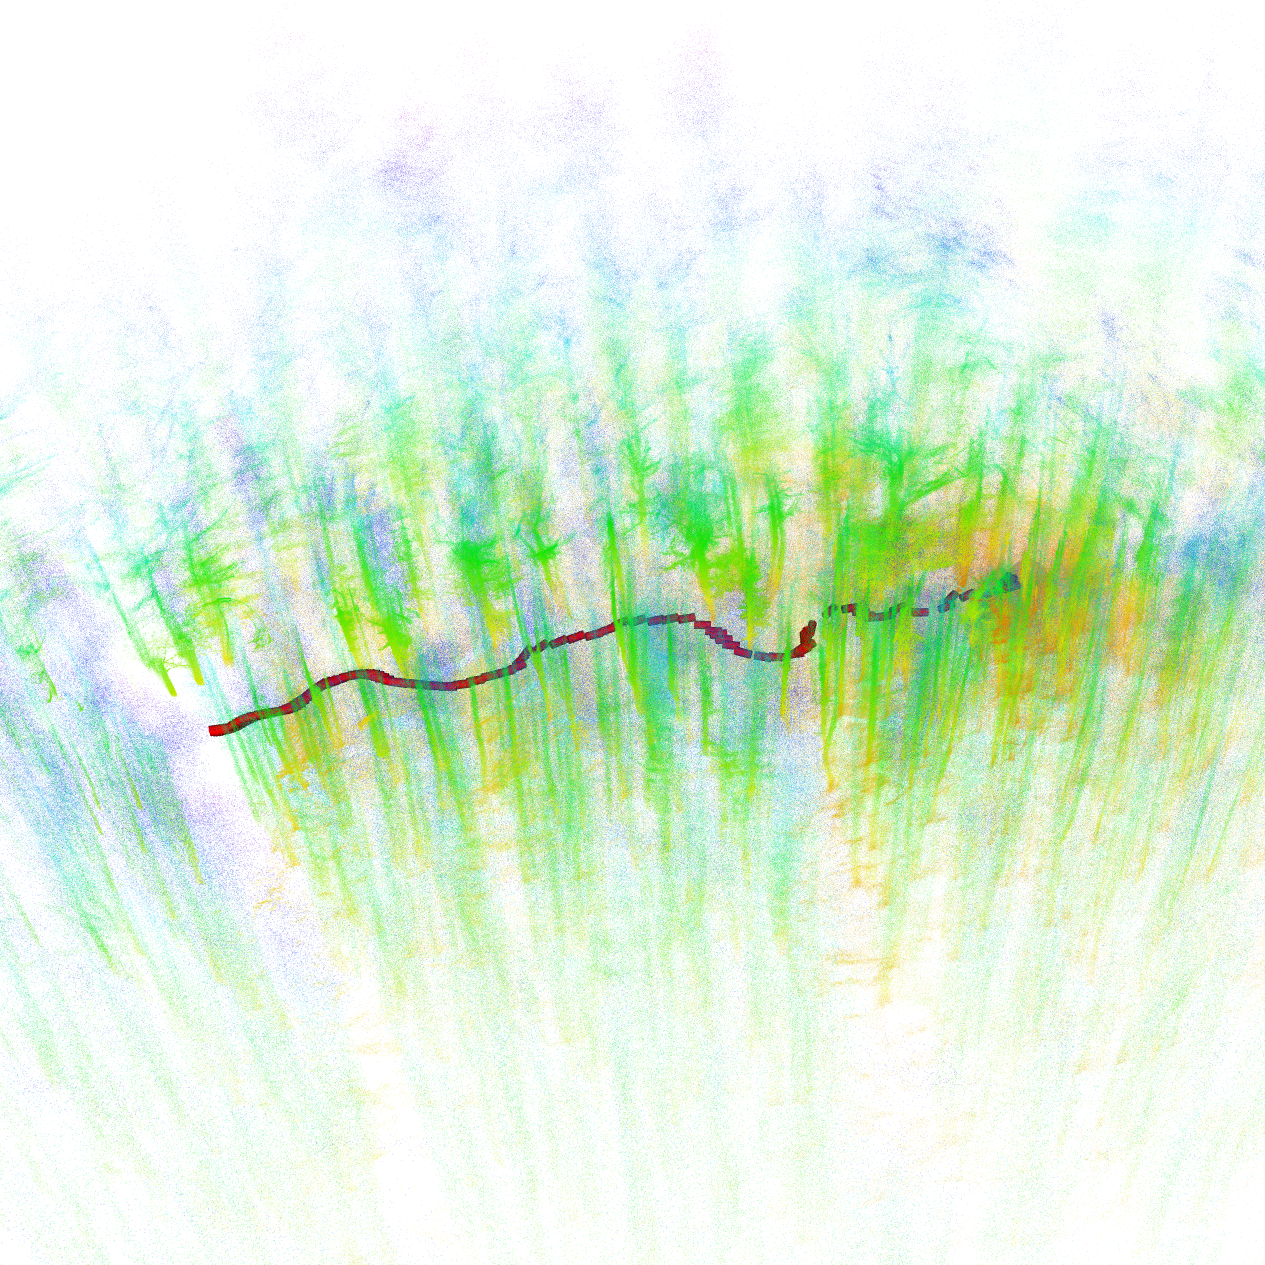
\includegraphics[width=0.48\textwidth]{./fig/rviz/flight_484.png}
                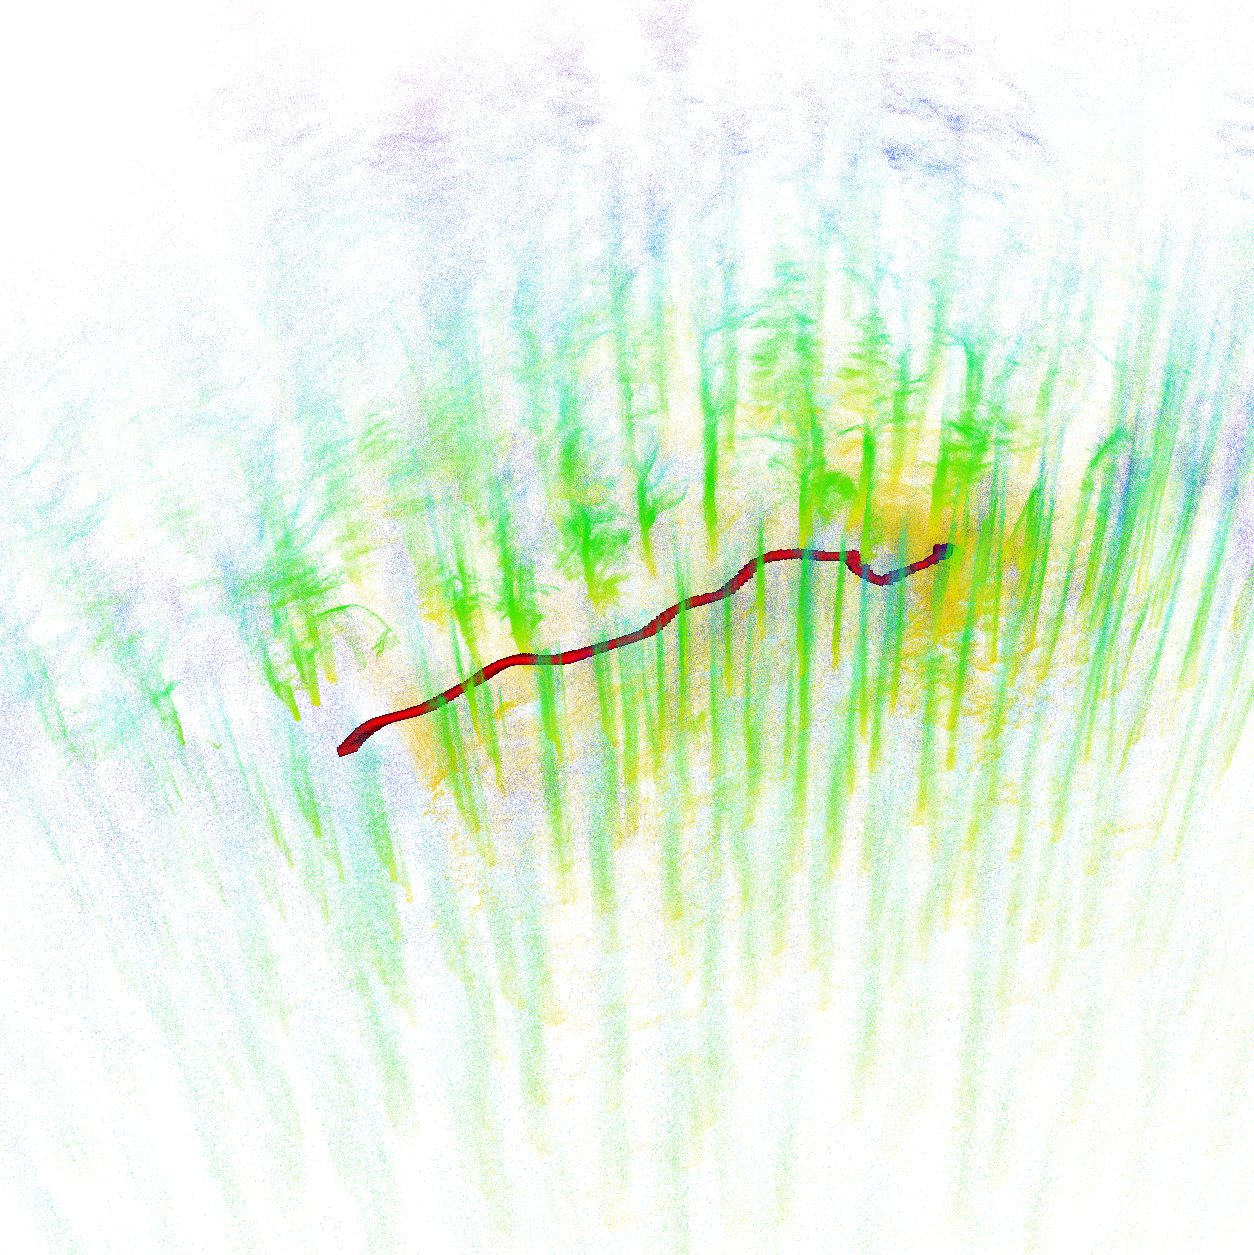
\includegraphics[width=0.48\textwidth]{./fig/rviz/flight_486.png}
                \caption{
                    \ac{UAV} flight trajectories through the forest test environment under different navigation settings. Left: Conservative parameter settings. Right: Aggressive parameter settings.
                }
                \label{fig:rbl_forest_conservative_flight_path}
            \end{figure}

        \subsection{Comparative Analysis}
            The real-world flight experiments conducted in the forest environment successfully validated the navigation capabilities of the proposed setup.
            The \ac{UAV} generally performed as expected based on simulation results, demonstrating its ability to navigate autonomously between points A and B while avoiding static obstacles.

            \subsection{Performance and Limitations}
                A primary limitation observed during real-world testing originated from the environmental mapping component, specifically the Bonxai mapping package used.
                While effective for static elements, the system occasionally struggled with dynamic obstacles, such as moving leaves.
                These obstacles were sometimes included in the voxel grid map and, due to the map's update policy (configured conservatively for safety), were not always removed immediately even when no longer present. 
                This could lead to situations where the \ac{UAV} perceived itself as blocked (as shown in the failure case video \cite{flight_fail}), requiring the safety pilot to land. 
                Addressing this mapping behavior is crucial for future testing.

            \subsection{Comparison with 2D Baseline}
                % Direct comparison with other state-of-the-art 3D navigation methods is challenging due to the specific nature of the RBL-based approach. 
                A meaningful comparison can be made with the original 2D RBL implementation \cite{rbl_paper}. 
                The key differences lie in the sensing and dimensionality:
                \begin{itemize}
                    \item The 2D version relied on a 2D \ac{LiDAR} for planar obstacle detection and a separate optical distance measurement sensor to maintain a constant flight altitude. 
                    Remapping obstacles in 2D is often simpler.
                    \item The 3D implementation utilizes a 3D \ac{LiDAR} for perception in three dimensions and must actively manage altitude based on the perceived environment, treating the ground itself as an obstacle.
                \end{itemize}
                A notable behavior observed in the 3D tests was the \ac{UAV}'s tendency to initially increase altitude after takeoff, effectively moving away from the ground obstacle, before potentially descending again as it got closer to the goal. 
                This behavior highlights the algorithm's capability to manage its vertical position based on the 3D environment.
                Regarding computational efficiency, while the 3D \ac{RBL} algorithm inherently involves greater complexity than its 2D counterpart (needing more points for 3D cell representation and more computational power for their partitioning), it nonetheless demonstrated manageable efficiency throughout the simulations and real-world flights.
                Illustrative examples of successful flights showcasing different parameter settings (\href{https://www.youtube.com/watch?v=DFt222gnA_w&ab_channel=MichalKamler}{aggressive} vs. \href{https://www.youtube.com/watch?v=AJPk0yVCPUo&ab_channel=MichalKamler}{conservative}) are provided in \cite{aggressive_flight} and \cite{conservative_flight}.

            \subsection{Future Work}
                The mapping limitations highlight key areas for future work. Potential solutions include:
                \begin{itemize}
                    \item \textbf{Dynamic Obstacle Handling: }\\
                    Implementing techniques to segment and filter out dynamic objects from the map representation such as \cite{TRLO_good_mapping}.
                    \item \textbf{Reactive Navigation: }\\
                    Exploring strategies that rely more on direct sensor input for immediate obstacle avoidance, removing dependence on the map, though this introduces challenges in perceiving areas outside the current sensor view (e.g. behind the UAV).
                    \item \textbf{Map-Based Strategic Replanning:} \\
                    Future work could include developing a higher-level path replanner that leverages the collected map to navigate agents around crowded areas, thereby supplementing the \ac{RBL} algorithm's local collision avoidance and enhancing overall efficiency.
                    \item \textbf{Map Update Logic: }\\
                    Investigating alternative mapping packages or implementing mechanisms like voxel decay instead of mapping (where unoccupied voxels gradually fade if not persistently observed) into the existing framework. 
                    While probabilistic mapping should ideally handle this, the developmental stage of the Bonxai package currently limits this capability.
                \end{itemize}
                Resolving these mapping challenges, particularly the robust handling of dynamic elements, is a prerequisite for advancing to more complex multi-agent experiments utilizing only onboard lidar sensing.
    
    \section{Conclusion}
    \label{sec:conclusion_lidar}
        This chapter detailed the implementation and real-world validation of the \ac{RBL} algorithm, adapted for autonomous \ac{UAV} navigation within a cluttered, \ac{GNSS}-denied forest environment using onboard 3D \ac{LiDAR} sensing. 
        The primary objective was to implement \ac{RBL} principles with real-time perception, state estimation (\ac{Point-LIO}), and mapping (Bonxai) to achieve reliable point-to-point navigation.

        Key technical contributions included adapting the \ac{RBL} algorithm's cell partitioning to directly utilize voxelized map data created from processed \ac{LiDAR} point clouds. 
        Modifications were also introduced to effectively handle the practical limitations of a single \ac{LiDAR} sensor with a restricted vertical field of view, ensuring safe convergence by constraining movement based on the actively sensed area while still leveraging map information. 
        An alternative approach using surface reconstruction via mesh generation was investigated but considered unsuitable due to computational complexity on the \ac{UAV} onboard computer.

        The proposed solution's effectiveness was demonstrated through both simulation and real-world experiments conducted in a forest. 
        The \ac{UAV} successfully navigated between designated start and goal points, avoiding static obstacles like trees and adapting its altitude based on the \ac{LiDAR}'s perception. 

        Despite the overall success, the experiments identified a key limitation related to the Bonxai mapping package's handling of dynamic environmental elements, such as moving leaves, which occasionally led to navigation deadlocks. 
        This emphasizes the importance of robust mapping with dynamic obstacles.

        In conclusion, this chapter successfully demonstrated the practical application and feasibility of using a 3D \ac{RBL} algorithm integrated with \ac{LiDAR} sensing for autonomous \ac{UAV} navigation in a challenging forest setting. 
        This capability can be observed in these videos \cite{aggressive_flight}, \cite{conservative_flight}.





% \chapter{Researching on possible enhancements of the algorithm for example using neural networks or learning-based techniques.\label{chap:enhancements}}

tune the paramaters of RBL to suit 3D

I will have to read something first, but what I found is that I could try object detection and classification using models like \href{https://arxiv.org/abs/1612.00593}{PointNet}, \href{https://arxiv.org/abs/1706.02413}{PointNet++} or \href{https://arxiv.org/abs/1711.06396}{VoxelNet}

Pointcloud denoising

Segmentation of LiDAR data.
\href{https://www.ipb.uni-bonn.de/wp-content/papercite-data/pdf/milioto2019iros.pdf}{RangeNet++}, \href{https://arxiv.org/abs/2003.03653}{SalsaNext} to differentiate between terrain trees and free space

NN approaches for approximating point clouds with simple convex shapes:

\href{https://openaccess.thecvf.com/content_CVPR_2020/papers/Deng_CvxNet_Learnable_Convex_Decomposition_CVPR_2020_paper.pdf}{CvxNet: Learnable Convex Decomposition by Deng et al. (CVPR 2020)}

\href{https://arxiv.org/abs/2003.13834}{Label-Efficient Learning on Point Clouds using Approximate Convex Decompositions by Gadelha et al. (Arxiv 2020)}

\href{https://arxiv.org/abs/1911.12870}{Region Segmentation via Deep Learning and Convex Optimization by Sonntag and Morgenshtern (Arxiv 2019)}

\href{https://arxiv.org/abs/2203.05662}{Point Density-Aware Voxels for LiDAR 3D Object Detection}

%% --------------------------------------------------------------
%% |                         Conclusion                         |
%% --------------------------------------------------------------

%!TEX root = ../main.tex

\chapter{Conclusion\label{chap:conclusion}}

This thesis set out to address key challenges in autonomous \ac{UAV} operations. 
The work focused on two primary objectives: first, to extend the established two-dimensional \ac{RBL} algorithm for effective multi-agent coordination in three-dimensional space, introducing new rules to enhance its performance. 
Secondly validating the practical application of this extended framework for single  \ac{UAV} navigation in a complex, GNSS-denied forest environment using onboard \ac{LiDAR} sensing.

The core contributions of this work began with the successful extension of the \ac{RBL} algorithm to 3D. 
This involved key modifications such as adapting Voronoi cell partitioning for three dimensions, modifying existing rules, and introducing a new elevation rotation angle designed to adjust the agent's vertical destination and improve spatial distribution. 
Simulations of multi-agent scenarios, including crossing circle and sphere formations, demonstrated that these extensions successfully enabled coordination in three dimensions. 
Notably, analysis revealed a trend where the performance advantage of the 3D \ac{RBL} approach with these rules, compared to the basic 2D version, increased with the number of agents.

Building upon this, the second major contribution was the practical implementation and real-world validation of the 3D \ac{RBL} algorithm for single  \ac{UAV} navigation. 
This involved integrating the algorithm with \ac{LiDAR}-based perception, Point-LIO for state estimation, and the Bonxai voxel-based mapping. 
Key technical advancements included adapting the \ac{RBL} cell partitioning to directly utilize voxelized map data and implementing software modifications to effectively handle the practical limitations of a single \ac{LiDAR} sensor with a restricted vertical field of view, ensuring safe movement based on actively sensed areas while still leveraging map information. 
Real-world experiments in a forest environment successfully demonstrated the  \ac{UAV}'s ability to navigate autonomously between designated start and goal points, avoiding static obstacles like trees and adapting its altitude based on \ac{LiDAR} perception, as shown in the provided flight videos \cite{aggressive_flight}, \cite{conservative_flight}.

The significance of these findings lies in advancing decentralized, rule-based control strategies for \ac{UAV}s operating in three dimensions. 
The successful 3D extension of \ac{RBL} offers a scalable approach for multi-agent systems, while the demonstration of \ac{LiDAR}-based navigation in a real forest highlights the potential for autonomous operations in GPS-denied settings. 

However, the research also identified limitations. 
For the multi-agent 3D \ac{RBL}, while simulations indicated advantages, the degree of improvement was occasionally less noticeable, possibly a result of conservative motion constraints and parameter settings that could be refined through further tuning.
The algorithm also requires an initial shared frame of reference for certain directional rules to function optimally. 
In the single-agent forest navigation, the primary challenge encountered was Bonxai mapping package, particularly its handling of dynamic environmental elements like moving leaves, which occasionally led to navigation deadlocks \cite{flight_fail}. 
This highlights the dependence of the current navigation approach on an accurate map representation.

Future work should therefore focus on improving the system's ability to handle dynamic obstacles. 
This could involve implementing another mapping algorithm or more sophisticated map update and filtering techniques, or by developing strategies that allow the UAV to react more directly to sensor perceptions of the environment, reducing dependence on map.

In conclusion, this thesis has successfully demonstrated the extension of the \ac{RBL} algorithm to 3D for multi-agent coordination in simulation and its practical application for single \ac{UAV} navigation in a real-world environment using \ac{LiDAR}. 
While challenges, particularly in perception and mapping in dynamic settings, remain, the presented work provides a valuable contribution and a solid foundation for future advancements in autonomous, rule-based \ac{UAV} navigation and coordination.


%% --------------------------------------------------------------
%% |                         References                         |
%% --------------------------------------------------------------

\chapter{References}

\printbibliography[heading=none,title={}]

%% --------------------------------------------------------------
%% |                         Appendices                         |
%% --------------------------------------------------------------

\appendix
\renewcommand\chaptername{Appendix}

\renewcommand{\thechapter}{A}
\renewcommand\chaptername{Appendix A}
\chapter{Experimental Results}
    \label{chap:exp_sim_res}
    \begin{itemize}
        \item \textbf{$N = 5$ Circular Formation:}
            \begin{table}[H]
                \centering
                \renewcommand{\arraystretch}{1.2}
                \begin{tabular}{|l|c|c|c|c|c|}
                \hline
                                            & \( SR \ [\%] \) & \( \overline{L} \ [\mathrm{m}] \) & \( \overline{t} \ [\mathrm{s}] \) & \( \overline{t}_{\text{max}} \ [\mathrm{s}] \) & \( \overline{v} \ [\mathrm{m/s}] \)     \\ \hline
                RBL \ac{2D}                      & 100.00          & 21.06 $\pm$ 0.10                  & 25.15 $\pm$ 0.21                  & 25.15 $\pm$ 0.19                               & 0.83 $\pm$ 0.01                         \\ \hline
                RBL \ac{3D}                      & 100.00          & 20.77 $\pm$ 0.29                  & 26.04 $\pm$ 0.51                  & 26.79 $\pm$ 0.27                               & 0.79 $\pm$ 0.02                         \\ \hline
                RBL \ac{3D}\(_{\text{clipped}}\) & 100.00          & 20.60 $\pm$ 0.24                  & 26.73 $\pm$ 0.47                  & 27.39 $\pm$ 0.28                               & 0.77 $\pm$ 0.02                         \\ \hline
                RBL \ac{3D}\(_z\)                & 100.00          & 20.97 $\pm$ 0.52                  & 25.54 $\pm$ 0.97                  & 26.72 $\pm$ 0.60                               & 0.81 $\pm$ 0.03                         \\ \hline
                \end{tabular}
            \end{table}
        \item \textbf{$N = 10$ Circular Formation:}
            \begin{table}[H]
                \centering
                \renewcommand{\arraystretch}{1.2}
                \begin{tabular}{|l|c|c|c|c|c|}
                \hline
                                            & \( SR \ [\%] \) & \( \overline{L} \ [\mathrm{m}] \) & \( \overline{t} \ [\mathrm{s}] \) & \( \overline{t}_{\text{max}} \ [\mathrm{s}] \) & \( \overline{v} \ [\mathrm{m/s}] \)     \\ \hline
                RBL \ac{2D}                      & 100.00          & 22.95 $\pm$ 1.64                  & 30.79 $\pm$ 2.28                  & 34.73 $\pm$ 0.77                               & 0.74 $\pm$ 0.07                         \\ \hline
                RBL \ac{3D}                      & 100.00          & 22.22 $\pm$ 0.89                  & 30.05 $\pm$ 2.61                  & 34.39 $\pm$ 4.19                               & 0.73 $\pm$ 0.05                         \\ \hline
                RBL \ac{3D}\(_{\text{clipped}}\) & 100.00          & 22.31 $\pm$ 0.69                  & 30.22 $\pm$ 1.83                  & 33.22 $\pm$ 0.93                               & 0.73 $\pm$ 0.04                         \\ \hline
                RBL \ac{3D}\(_z\)                & 100.00          & 22.38 $\pm$ 0.88                  & 28.80 $\pm$ 2.30                  & 32.35 $\pm$ 1.25                               & 0.77 $\pm$ 0.05                         \\ \hline
                \end{tabular}
            \end{table}
        \item \textbf{$N = 15$ Circular Formation:}
            \begin{table}[H]
                \centering
                \renewcommand{\arraystretch}{1.2}
                \begin{tabular}{|l|c|c|c|c|c|}
                \hline
                                            & \( SR \ [\%] \) & \( \overline{L} \ [\mathrm{m}] \) & \( \overline{t} \ [\mathrm{s}] \) & \( \overline{t}_{\text{max}} \ [\mathrm{s}] \) & \( \overline{v} \ [\mathrm{m/s}] \)     \\ \hline
                RBL \ac{2D}                      & 100.00          & 23.56 $\pm$ 1.75                  & 33.89 $\pm$ 2.48                  & 38.75 $\pm$ 1.45                               & 0.69 $\pm$ 0.06                         \\ \hline
                RBL \ac{3D}                      & 100.00          & 22.36 $\pm$ 0.97                  & 30.65 $\pm$ 3.07                  & 35.77 $\pm$ 3.72                               & 0.72 $\pm$ 0.07                         \\ \hline
                RBL \ac{3D}\(_{\text{clipped}}\) & 100.00          & 22.32 $\pm$ 0.81                  & 30.69 $\pm$ 2.61                  & 34.50 $\pm$ 0.47                               & 0.72 $\pm$ 0.06                         \\ \hline
                RBL \ac{3D}\(_z\)                & 100.00          & 22.64 $\pm$ 0.95                  & 29.67 $\pm$ 2.54                  & 34.27 $\pm$ 0.88                               & 0.76 $\pm$ 0.06                         \\ \hline
                \end{tabular}
            \end{table}
        \item \textbf{$N = 10$ Spherical Formation:}
            \begin{table}[H]
                \centering
                \renewcommand{\arraystretch}{1.2}
                \begin{tabular}{|l|c|c|c|c|c|}
                \hline
                                            & \( SR \ [\%] \) & \( \overline{L} \ [\mathrm{m}] \) & \( \overline{t} \ [\mathrm{s}] \) & \( \overline{t}_{\text{max}} \ [\mathrm{s}] \) & \( \overline{v} \ [\mathrm{m/s}] \)     \\ \hline
                RBL \ac{3D}                      & 100.00          & 14.32 $\pm$ 1.52                  & 27.76 $\pm$ 3.06                  & 32.48 $\pm$ 2.26                               & 0.51 $\pm$ 0.05                         \\ \hline
                RBL \ac{3D}\(_z\)                & 100.00          & 14.06 $\pm$ 0.97                  & 27.17 $\pm$ 2.66                  & 31.86 $\pm$ 1.24                               & 0.55 $\pm$ 0.06                         \\ \hline
                \end{tabular}
            \end{table}
    \end{itemize}

    \begin{figure}[H]
        \centering
        \subfloat[Top-Down View (X-Y)] {
        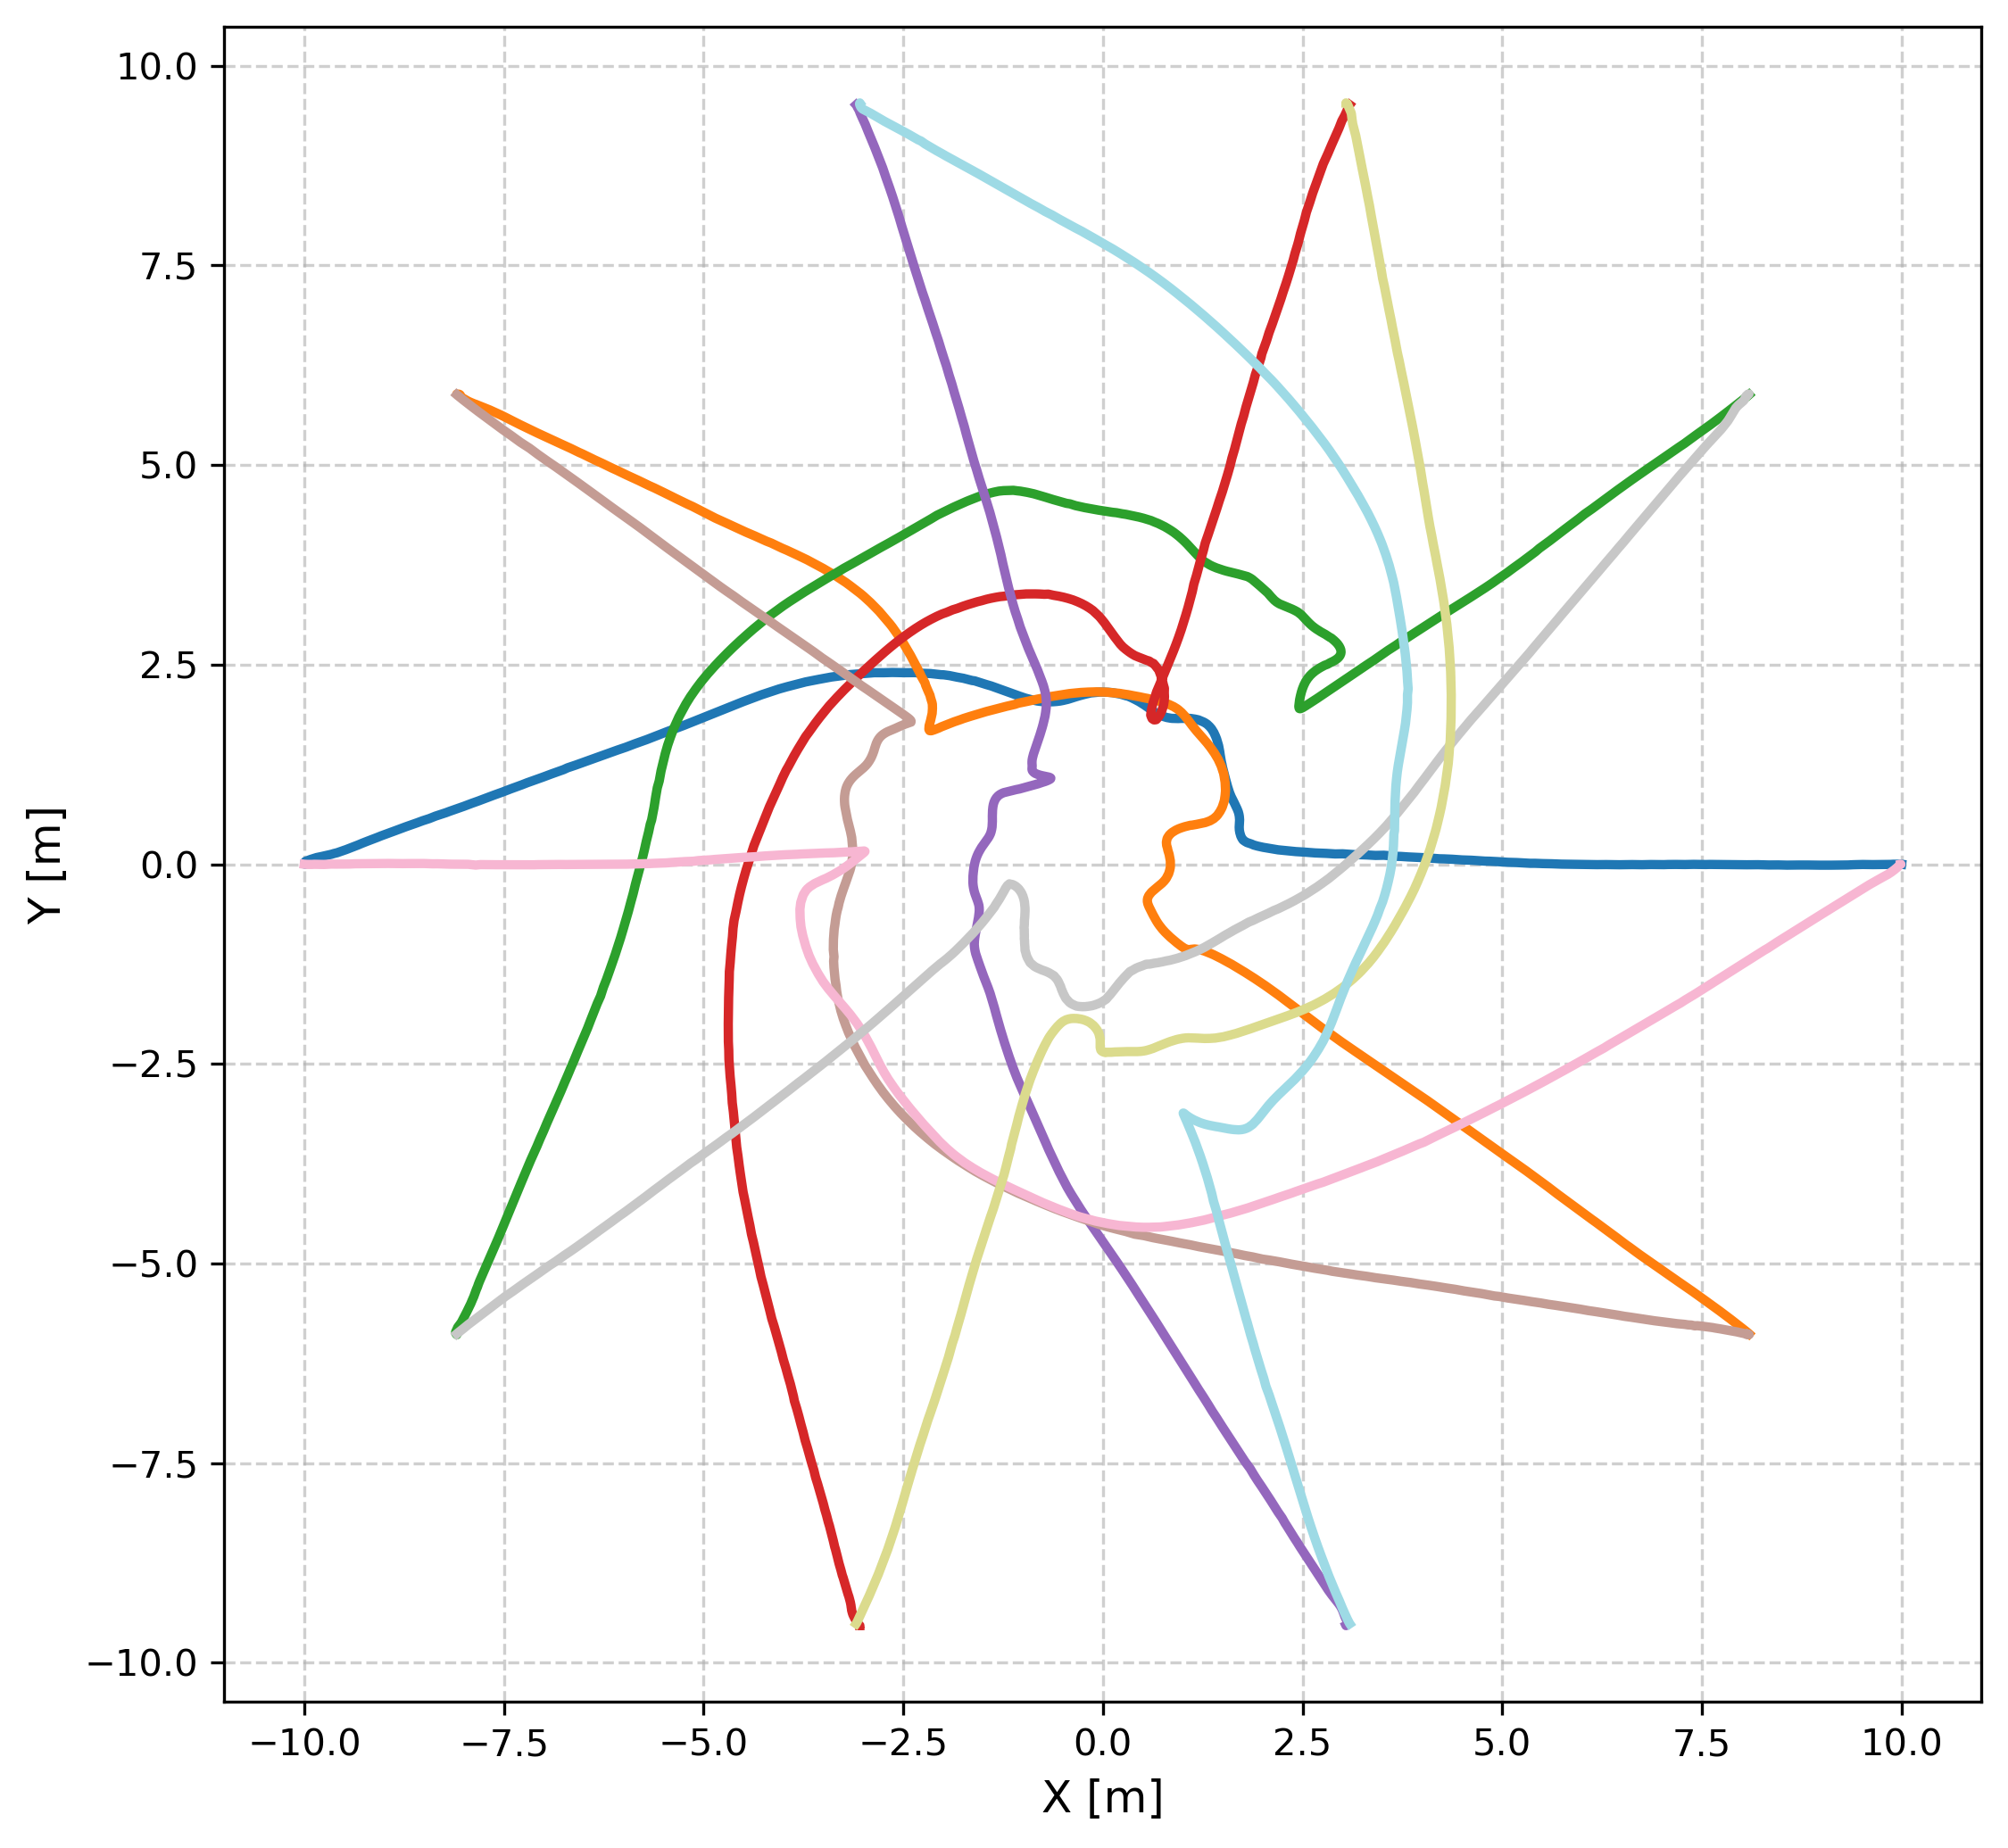
\includegraphics[width=0.48\textwidth, height=0.48\textwidth]{./fig/plots/circle_2d_top_down.png}
        }
        \subfloat[Side View (X-Z)] {
            \raisebox{0.12\textwidth}{
                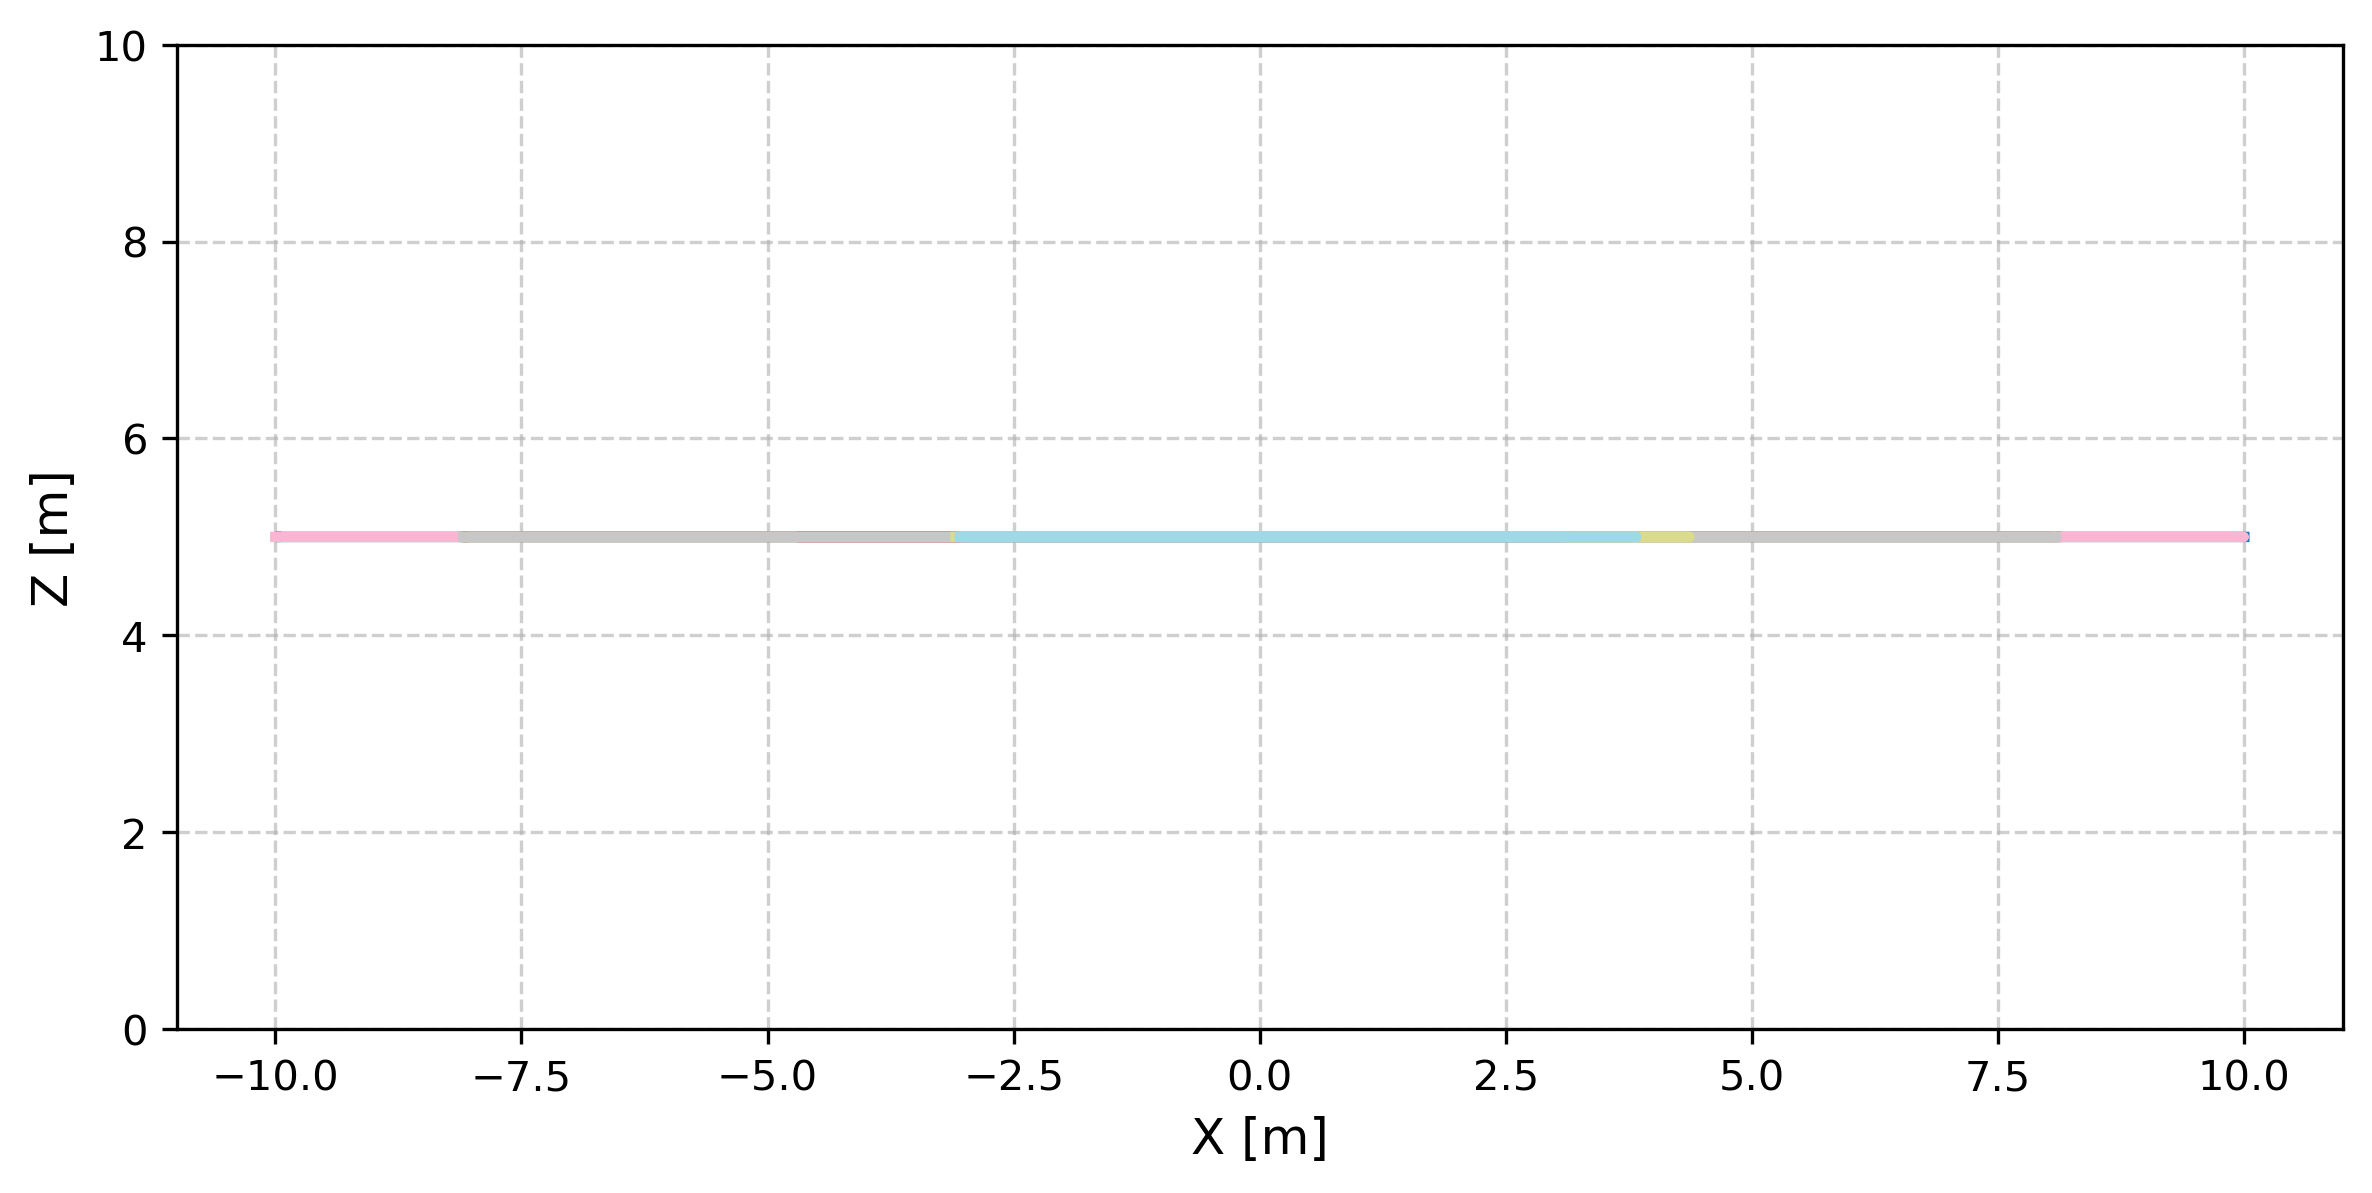
\includegraphics[width=0.48\textwidth, height=0.24\textwidth]{./fig/plots/circle_2d_side.png}
            }
        }
        \caption{
            Trajectories in a \ac{2D} circular crossing.
        }
        \label{}
    \end{figure}

    \begin{figure}[H]
        \centering
        \subfloat[Top-Down View (X-Y)] {
        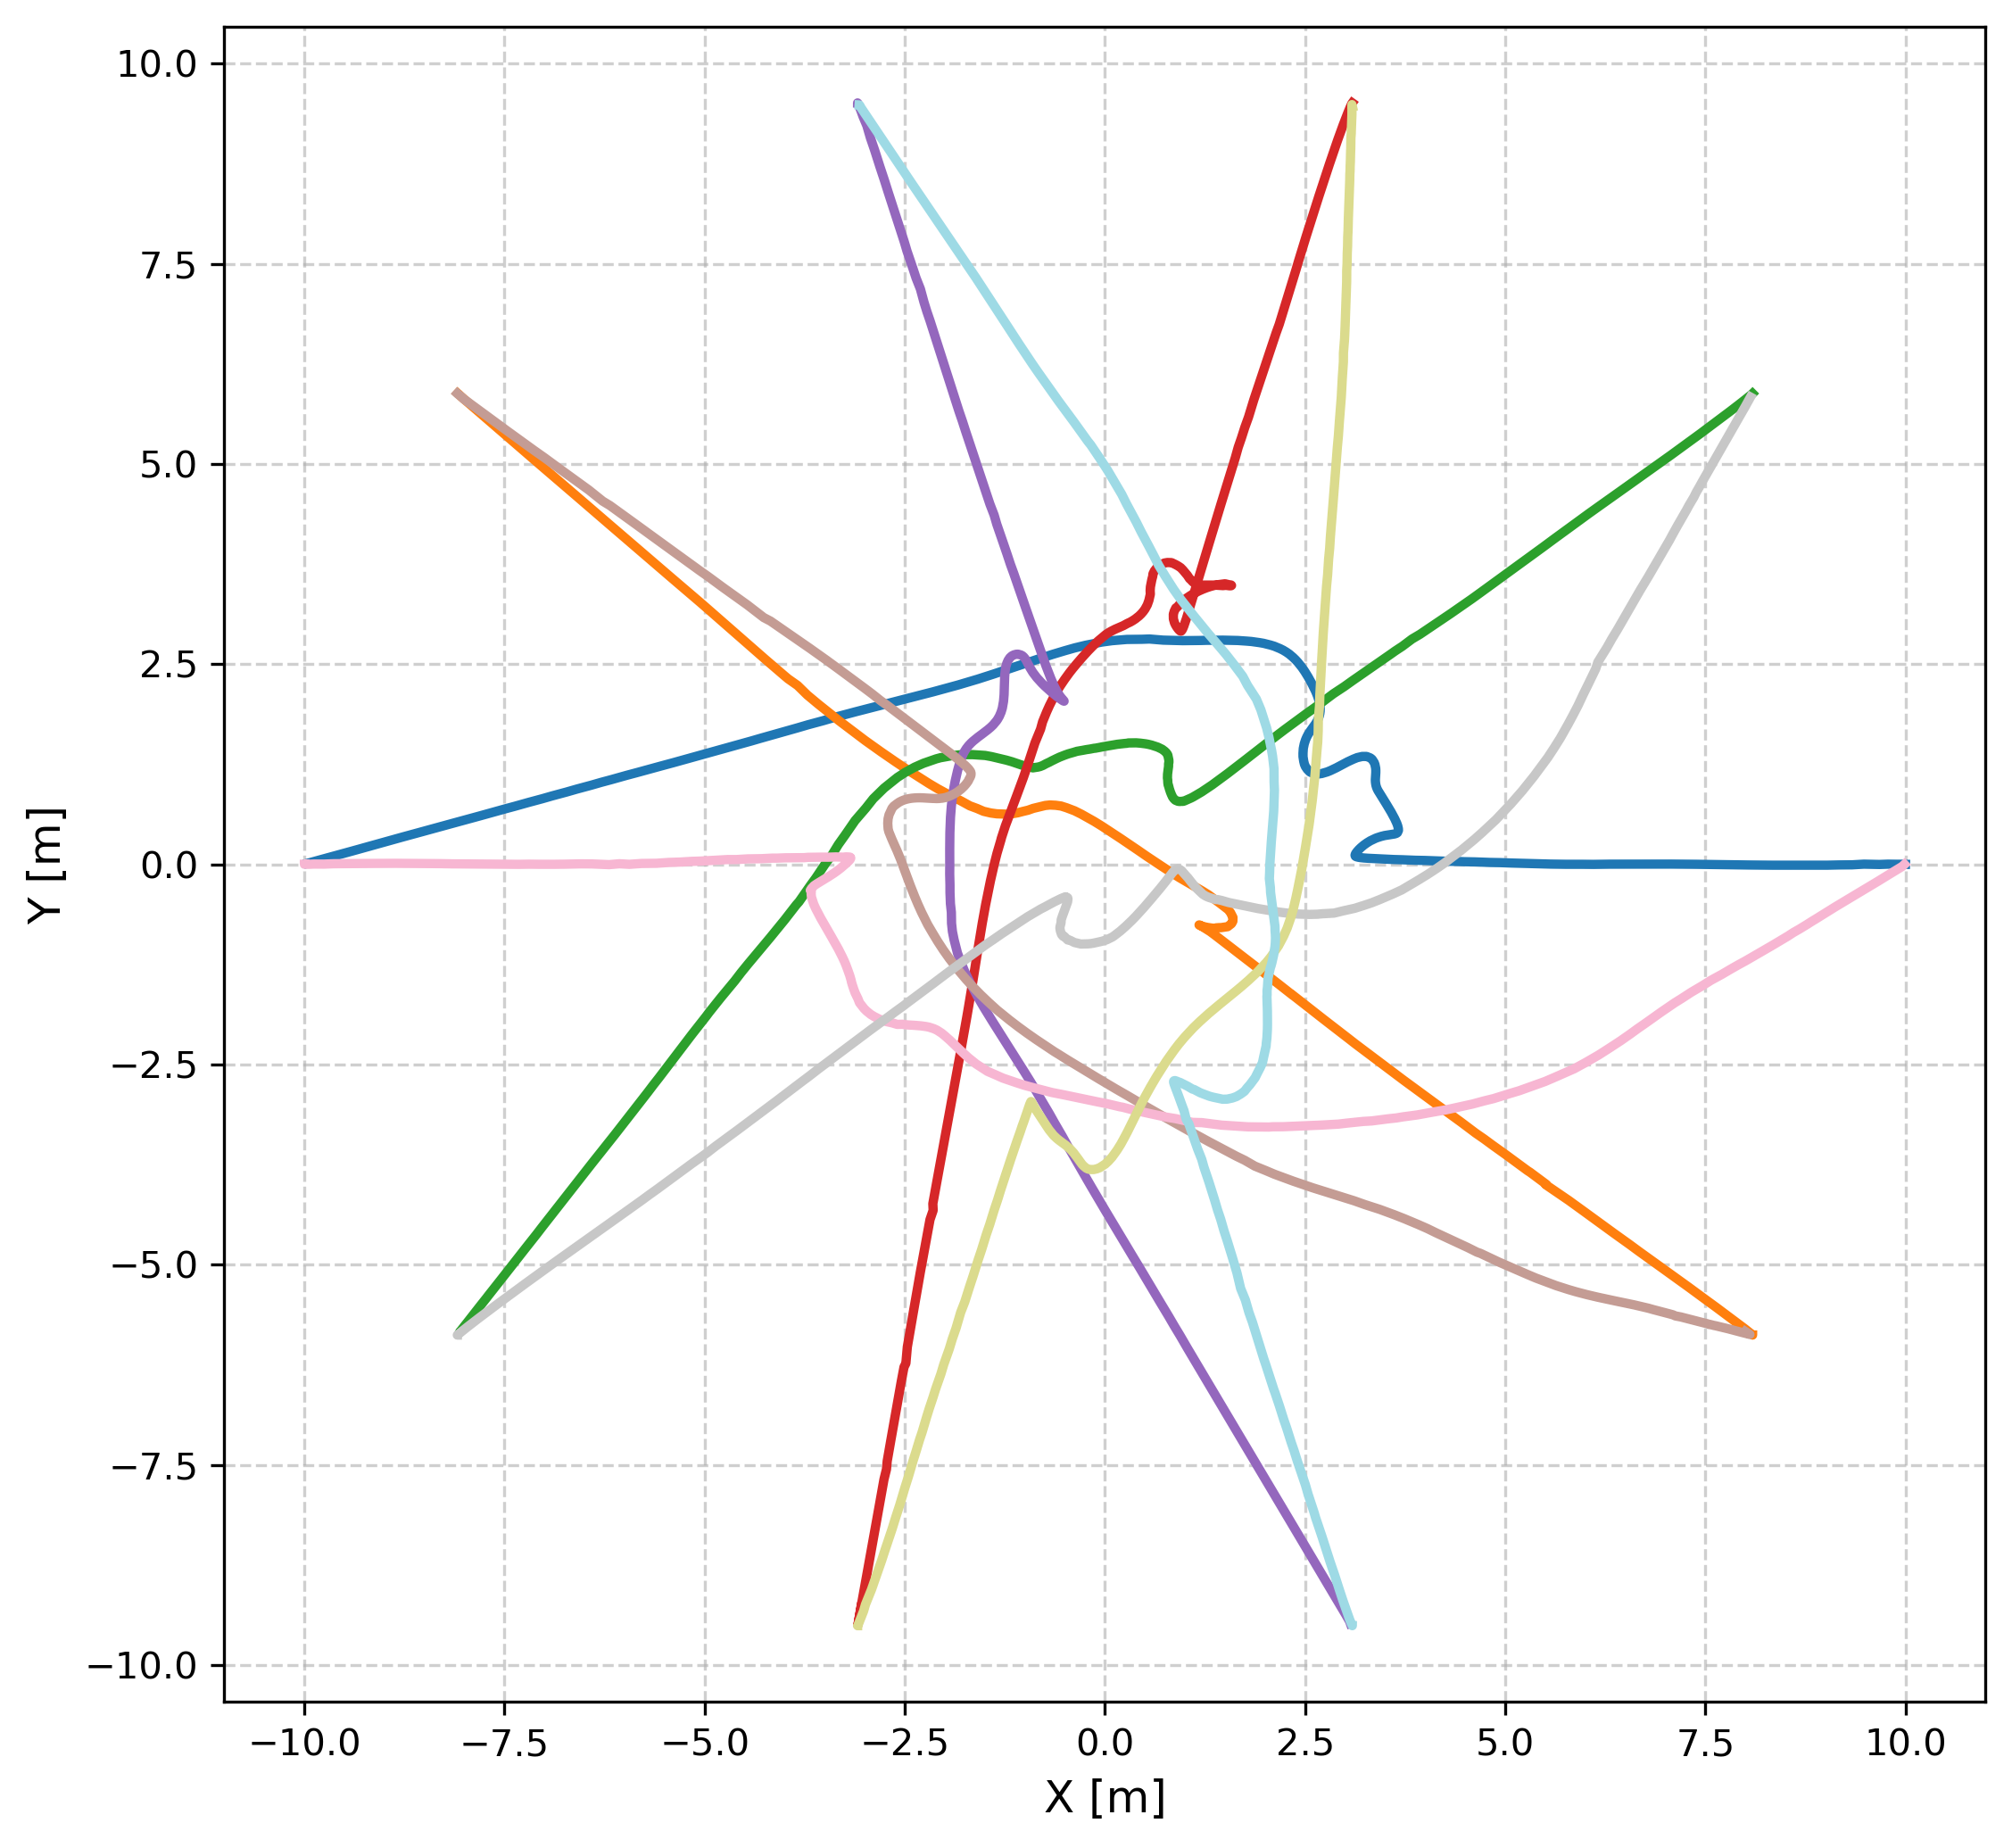
\includegraphics[width=0.48\textwidth, height=0.48\textwidth]{./fig/plots/circle_3d_top_down.png}
        }
        \subfloat[Side View (X-Z)] {
            \raisebox{0.12\textwidth}{
                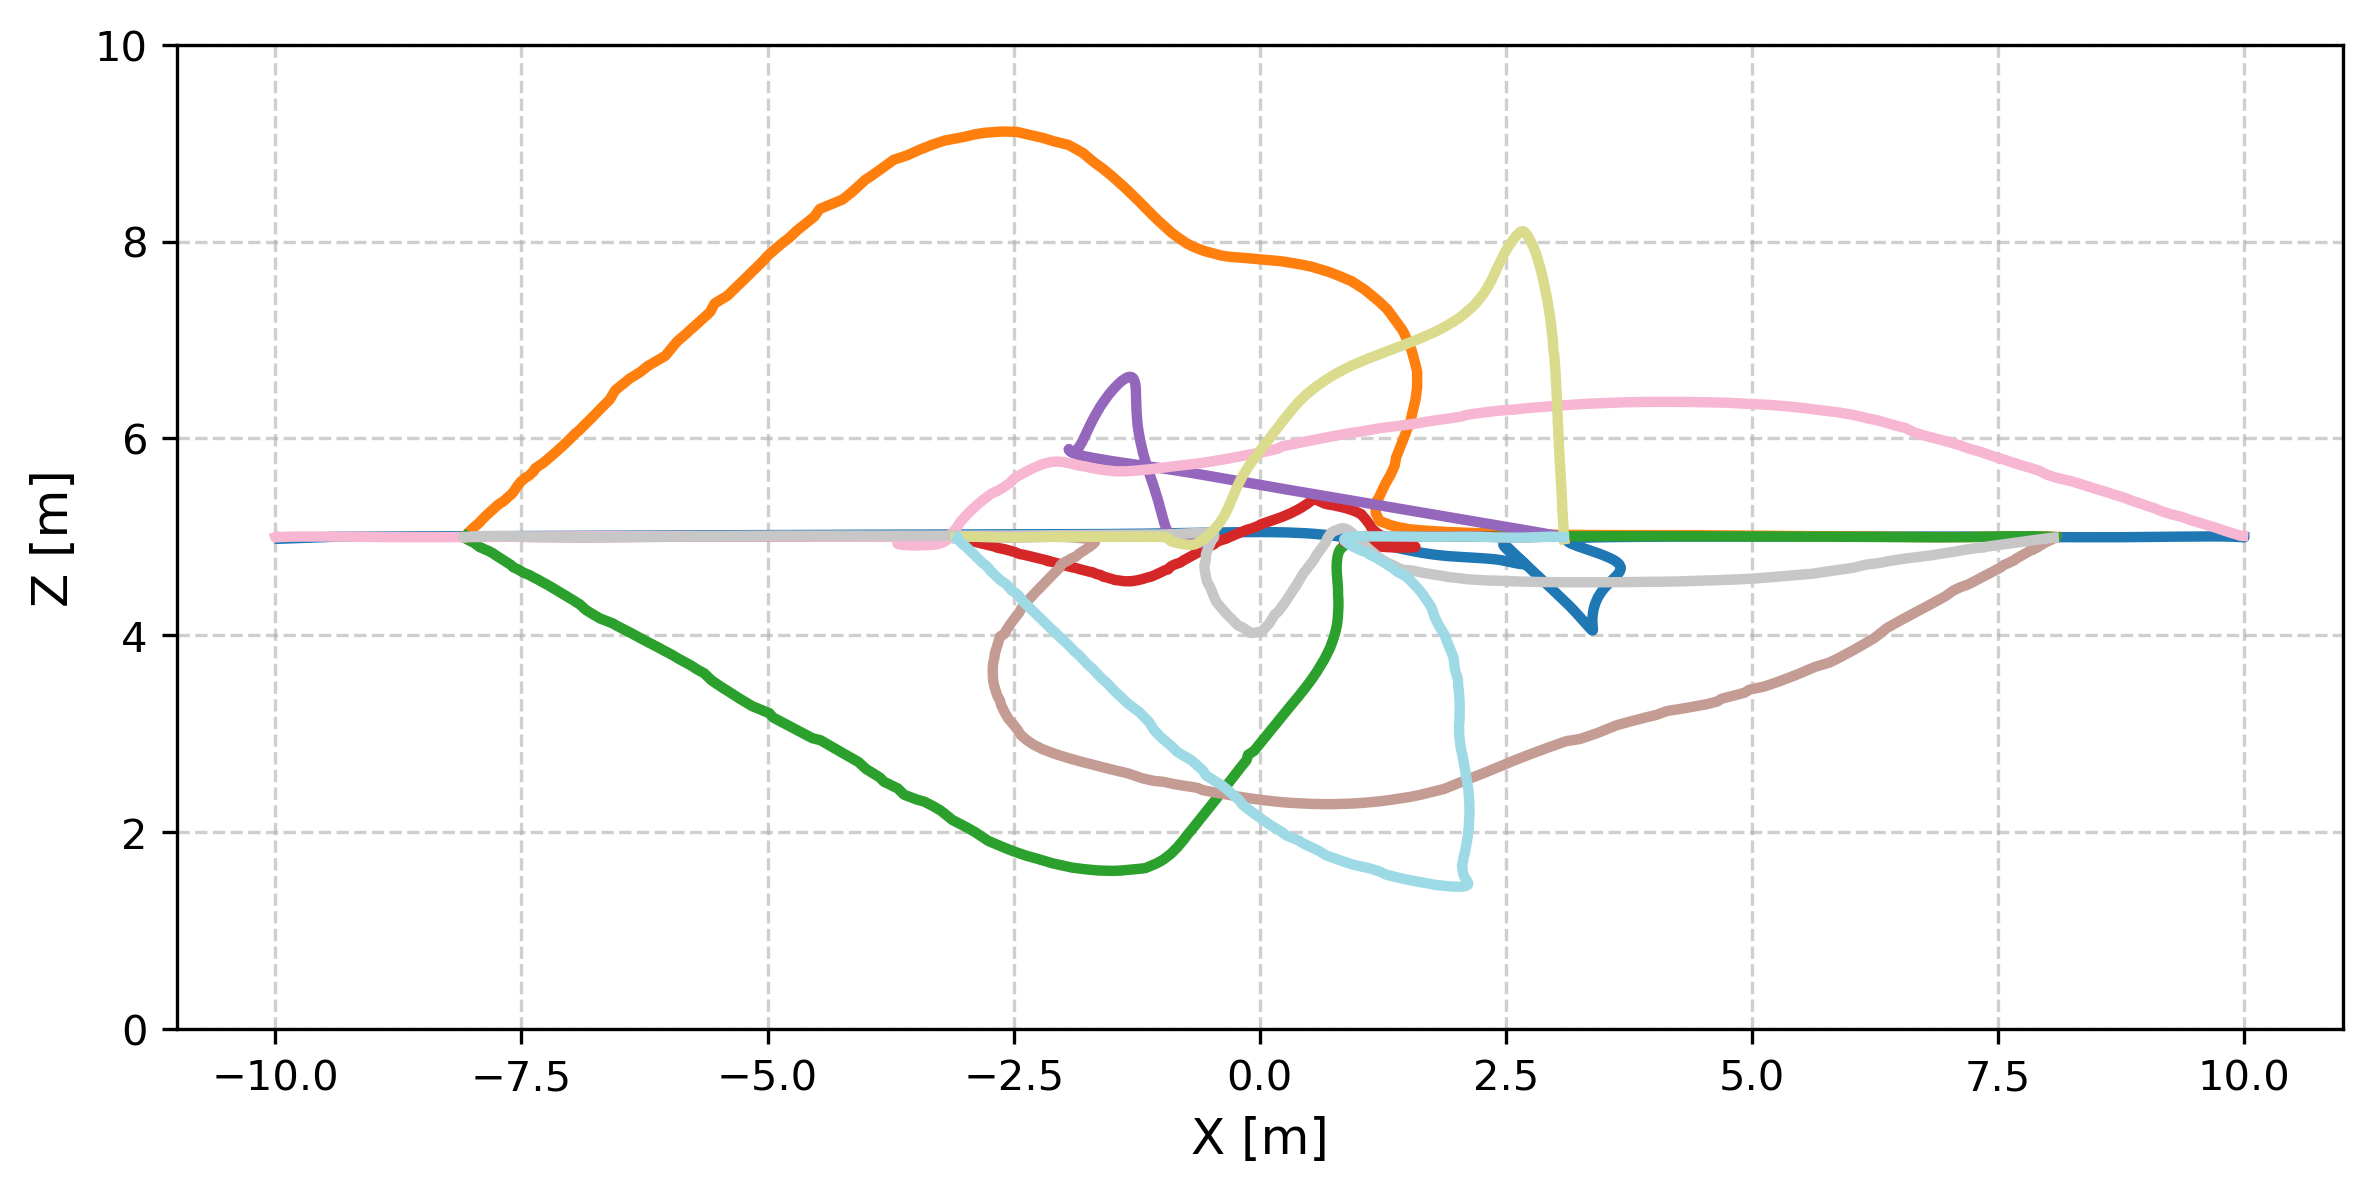
\includegraphics[width=0.48\textwidth, height=0.24\textwidth]{./fig/plots/circle_3d_side.png}
            }
        }
        \caption{
            Trajectories in a \ac{3D} circular crossing.
        }
        \label{}
    \end{figure}

    \begin{figure}[H]
        \centering
        \subfloat[Top-Down View (X-Y)] {
        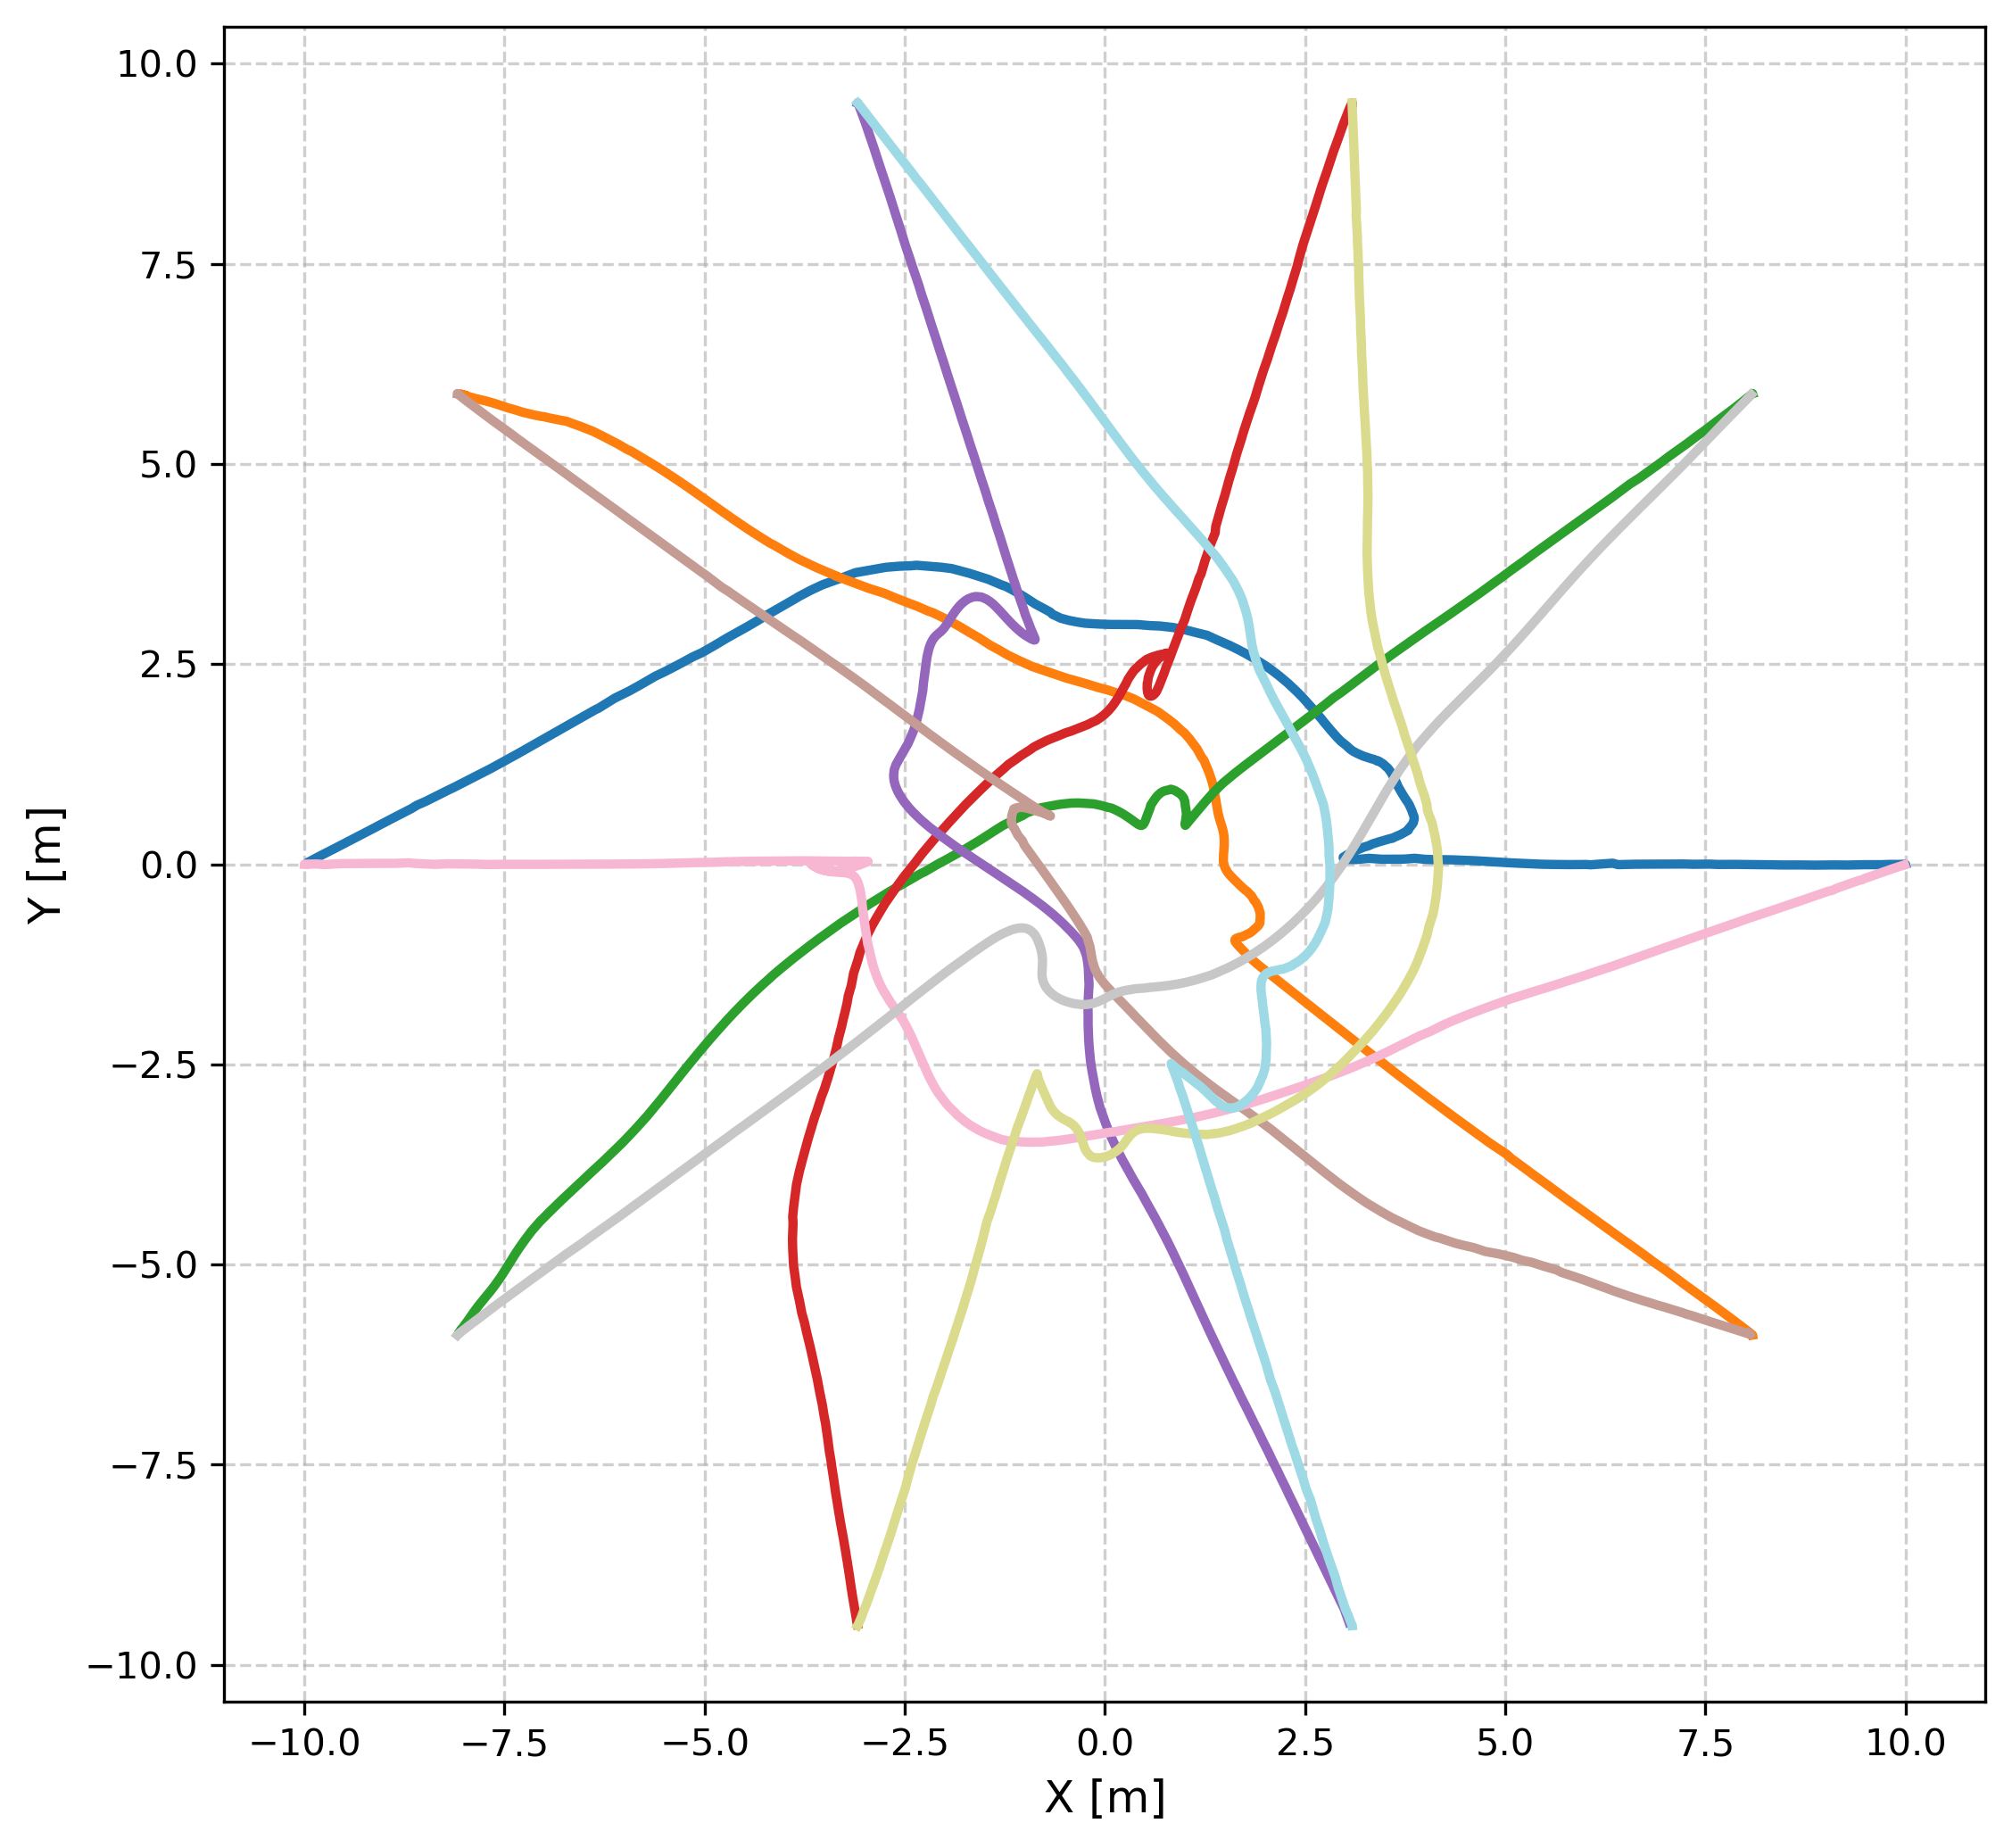
\includegraphics[width=0.48\textwidth, height=0.48\textwidth]{./fig/plots/circle_3d_z_clip_top_down.png}
        }
        \subfloat[Side View (X-Z)] {
            \raisebox{0.12\textwidth}{
                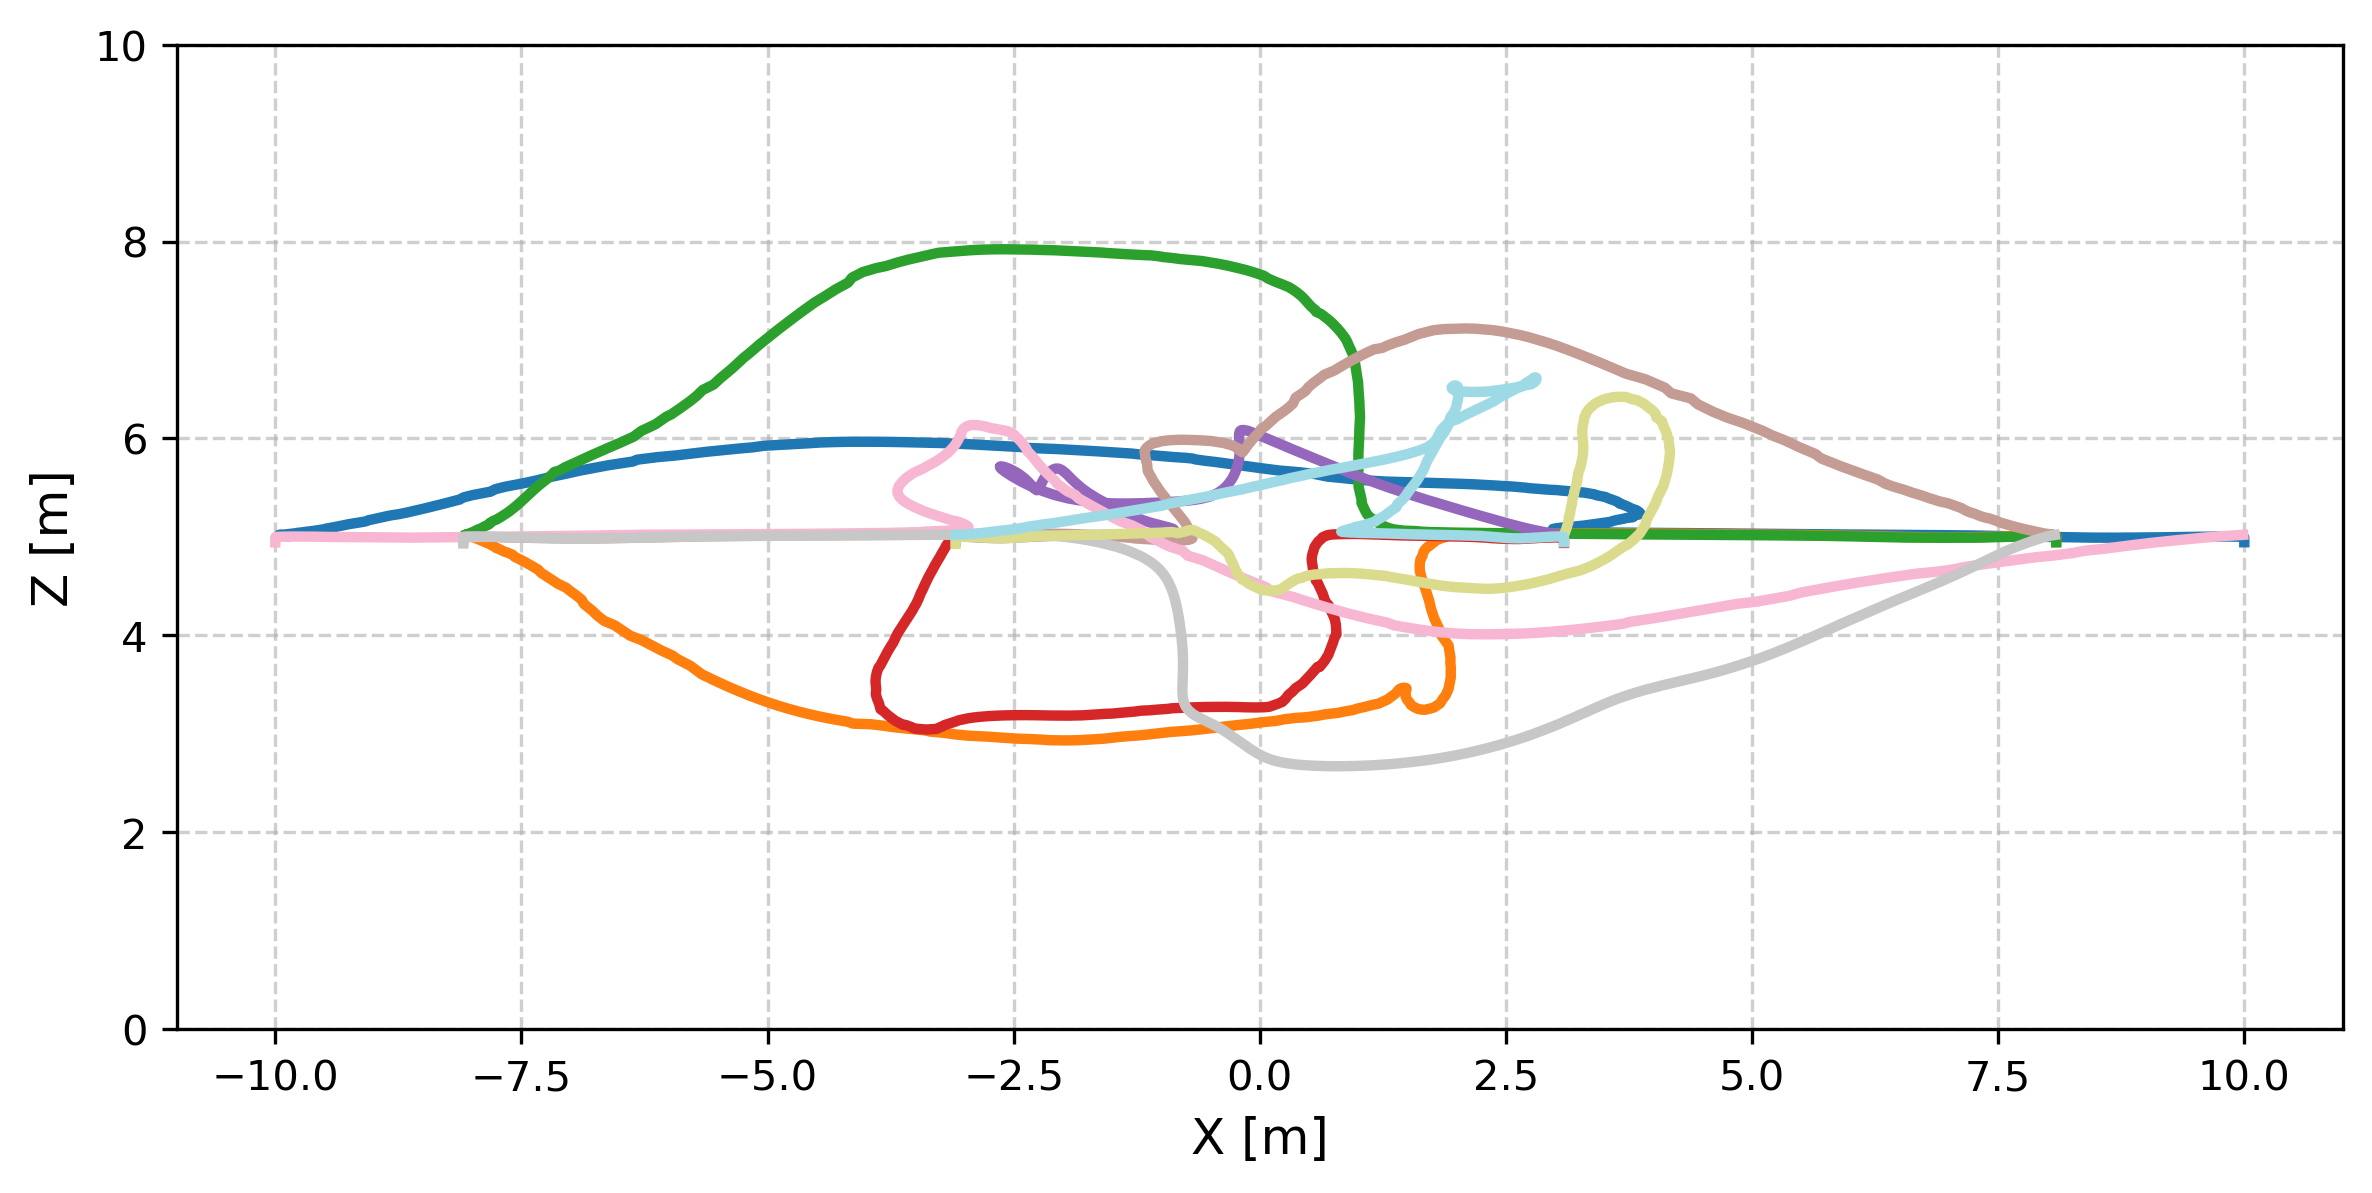
\includegraphics[width=0.48\textwidth, height=0.24\textwidth]{./fig/plots/circle_3d_z_clip_side.png}
            }
        }
        \caption{
            Effect of Z-axis clipping on the circular crossing.   
        }
        \label{}
    \end{figure}

    \begin{figure}[H]
        \centering
        \subfloat[Top-Down View (X-Y)] {
        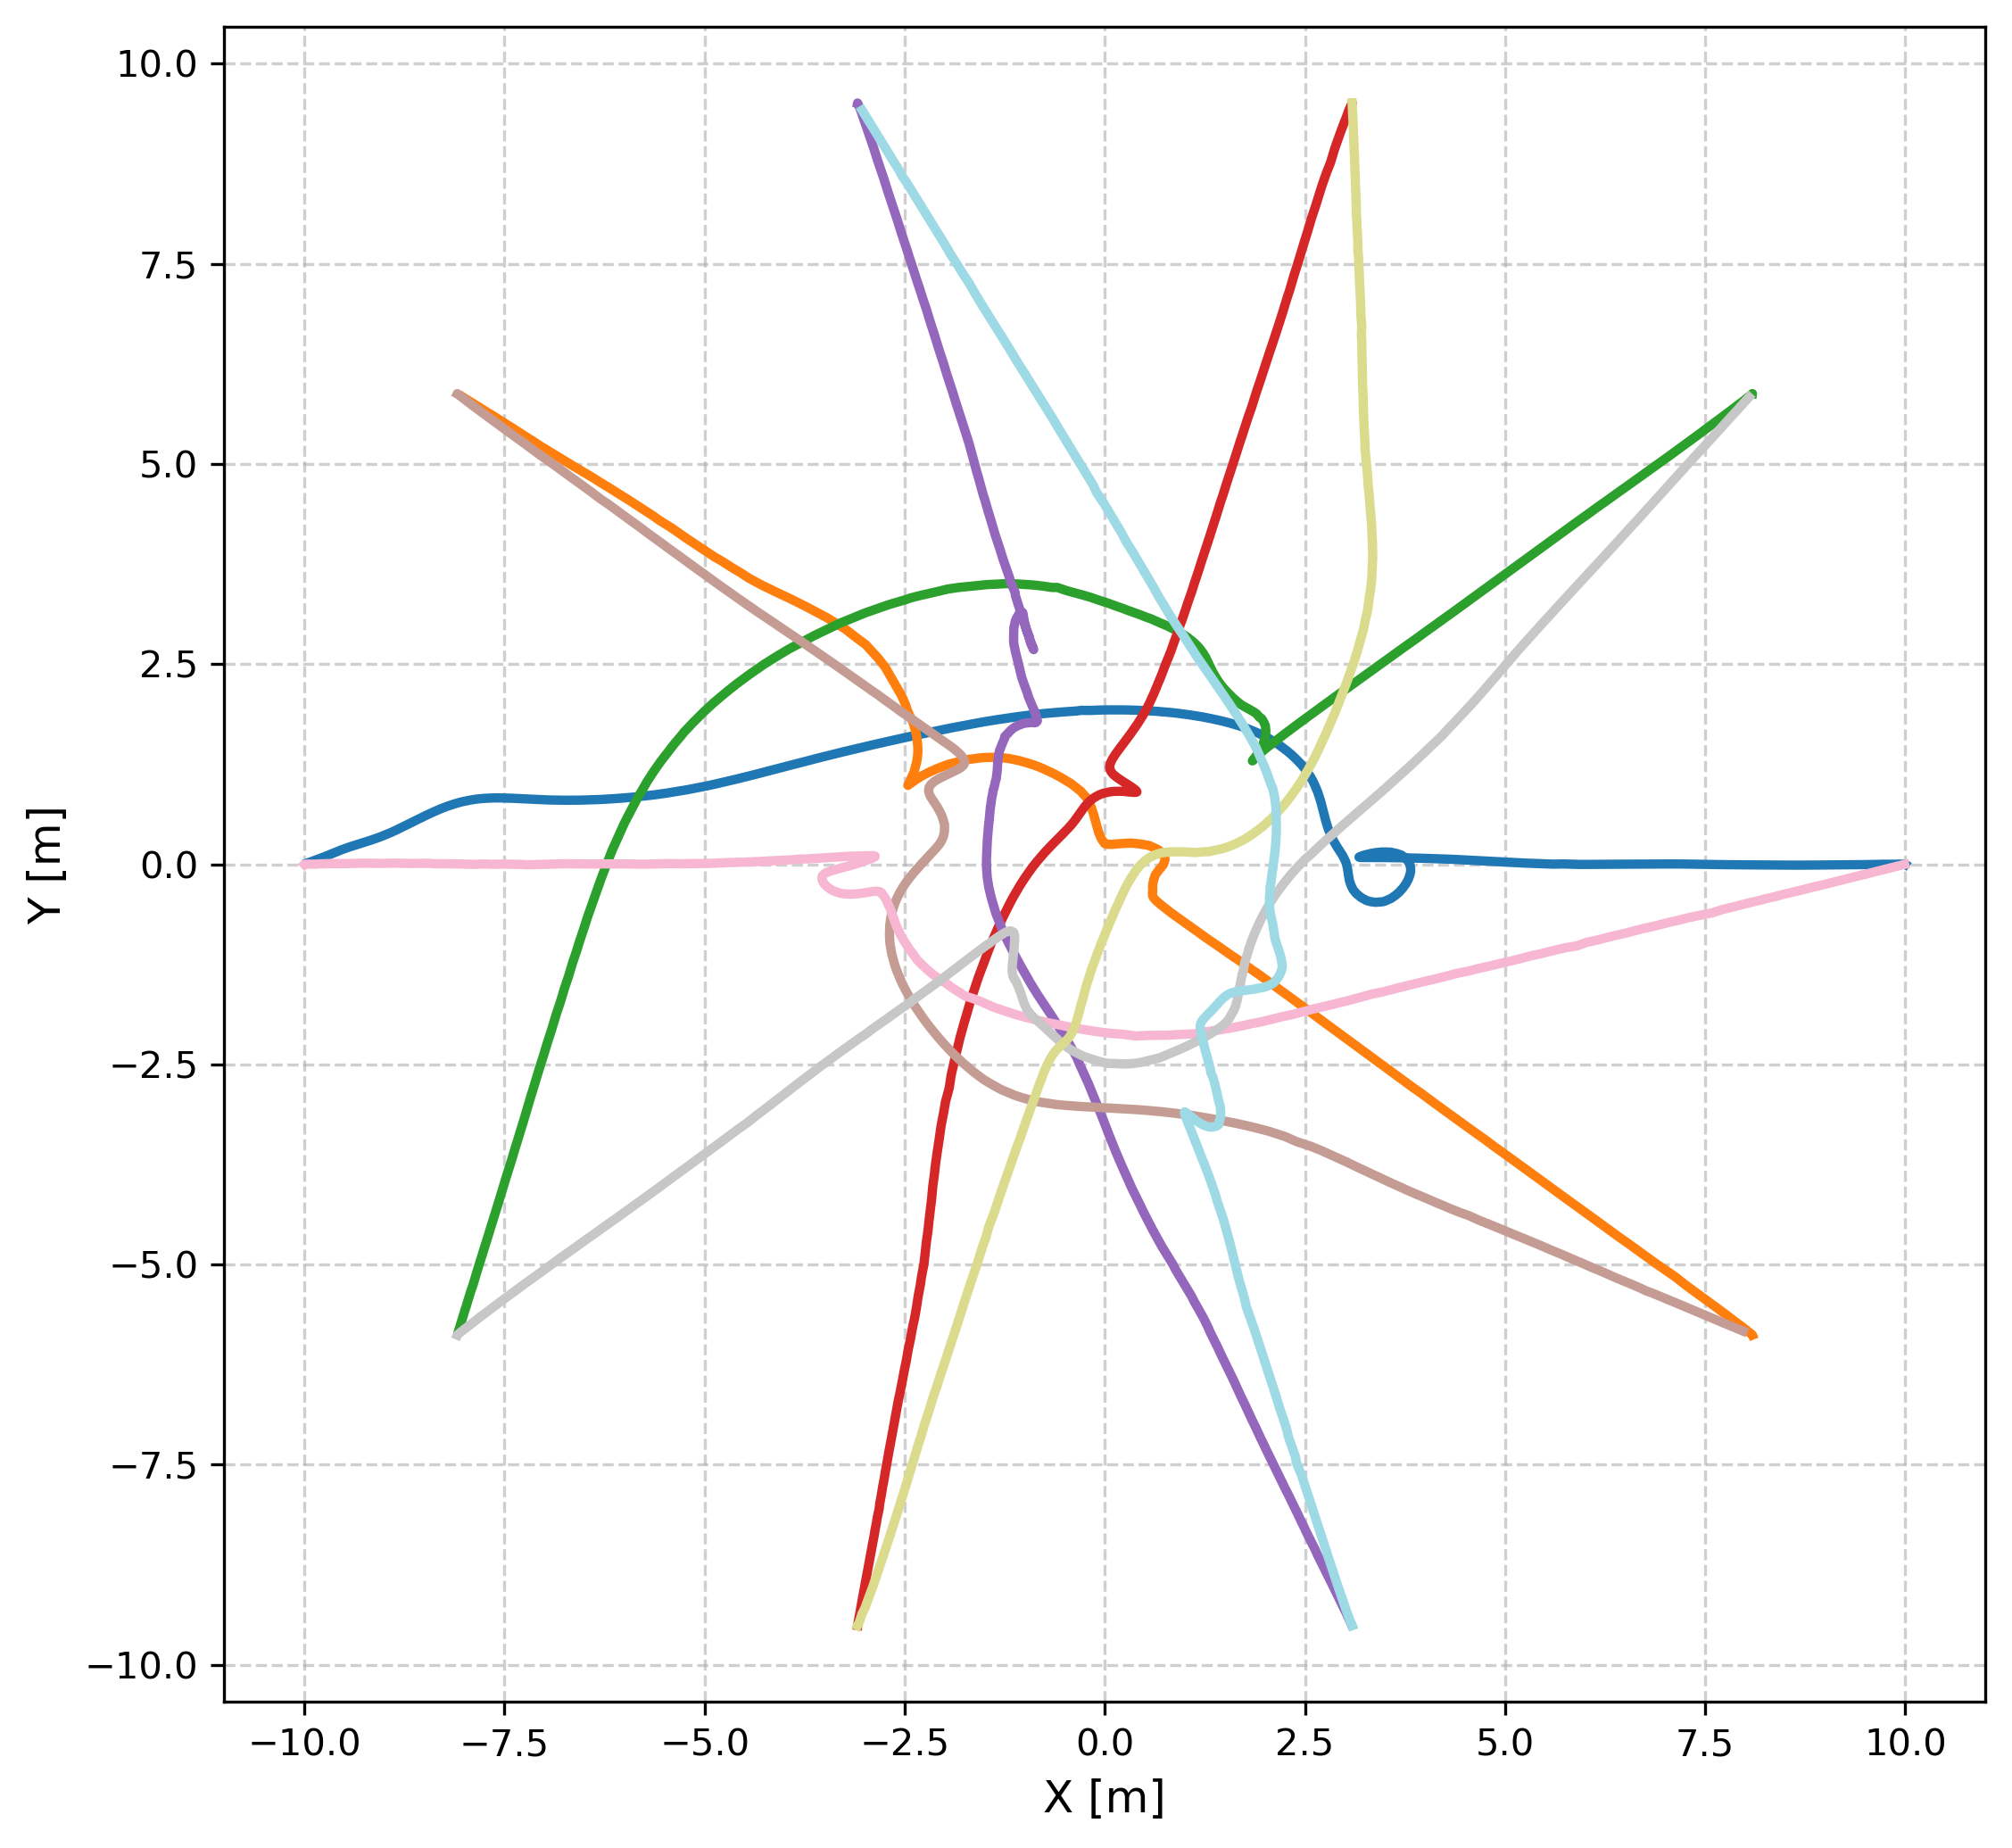
\includegraphics[width=0.48\textwidth, height=0.48\textwidth]{./fig/plots/circle_3d_z_rule_top_down.png}
        }
        \subfloat[Side View (X-Z)] {
            \raisebox{0.12\textwidth}{
                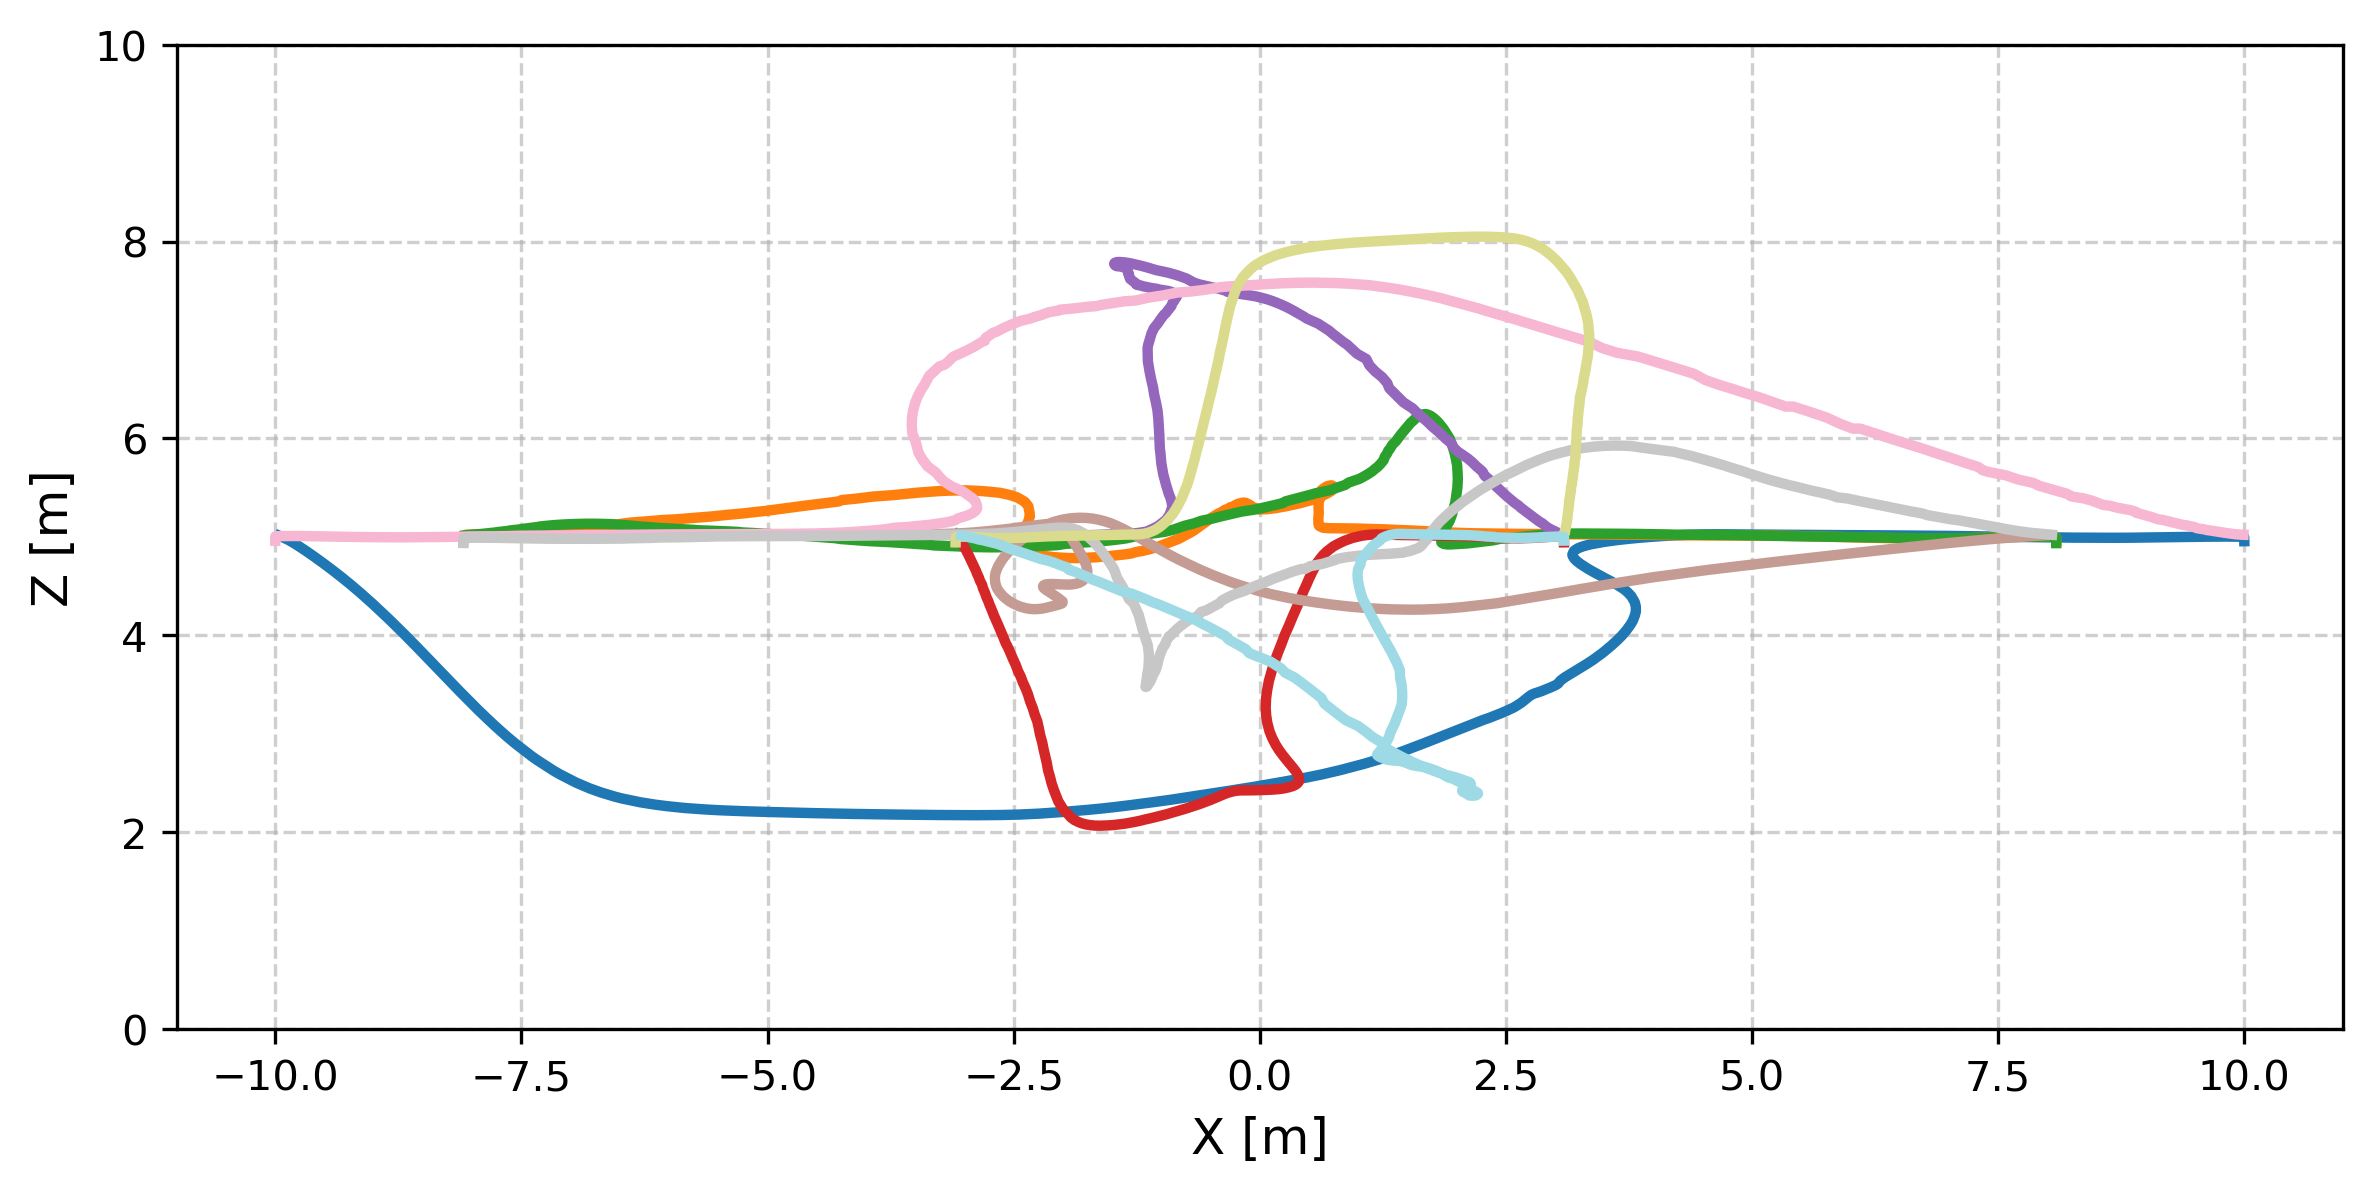
\includegraphics[width=0.48\textwidth, height=0.24\textwidth]{./fig/plots/circle_3d_z_rule_side.png}
            }
        }
        \caption{
            Effect of the Z-axis rule on the circular crossing. 
        }
        \label{}
    \end{figure}

    \begin{figure}[H]
        \centering
        \subfloat[Top-Down View (X-Y)] {
        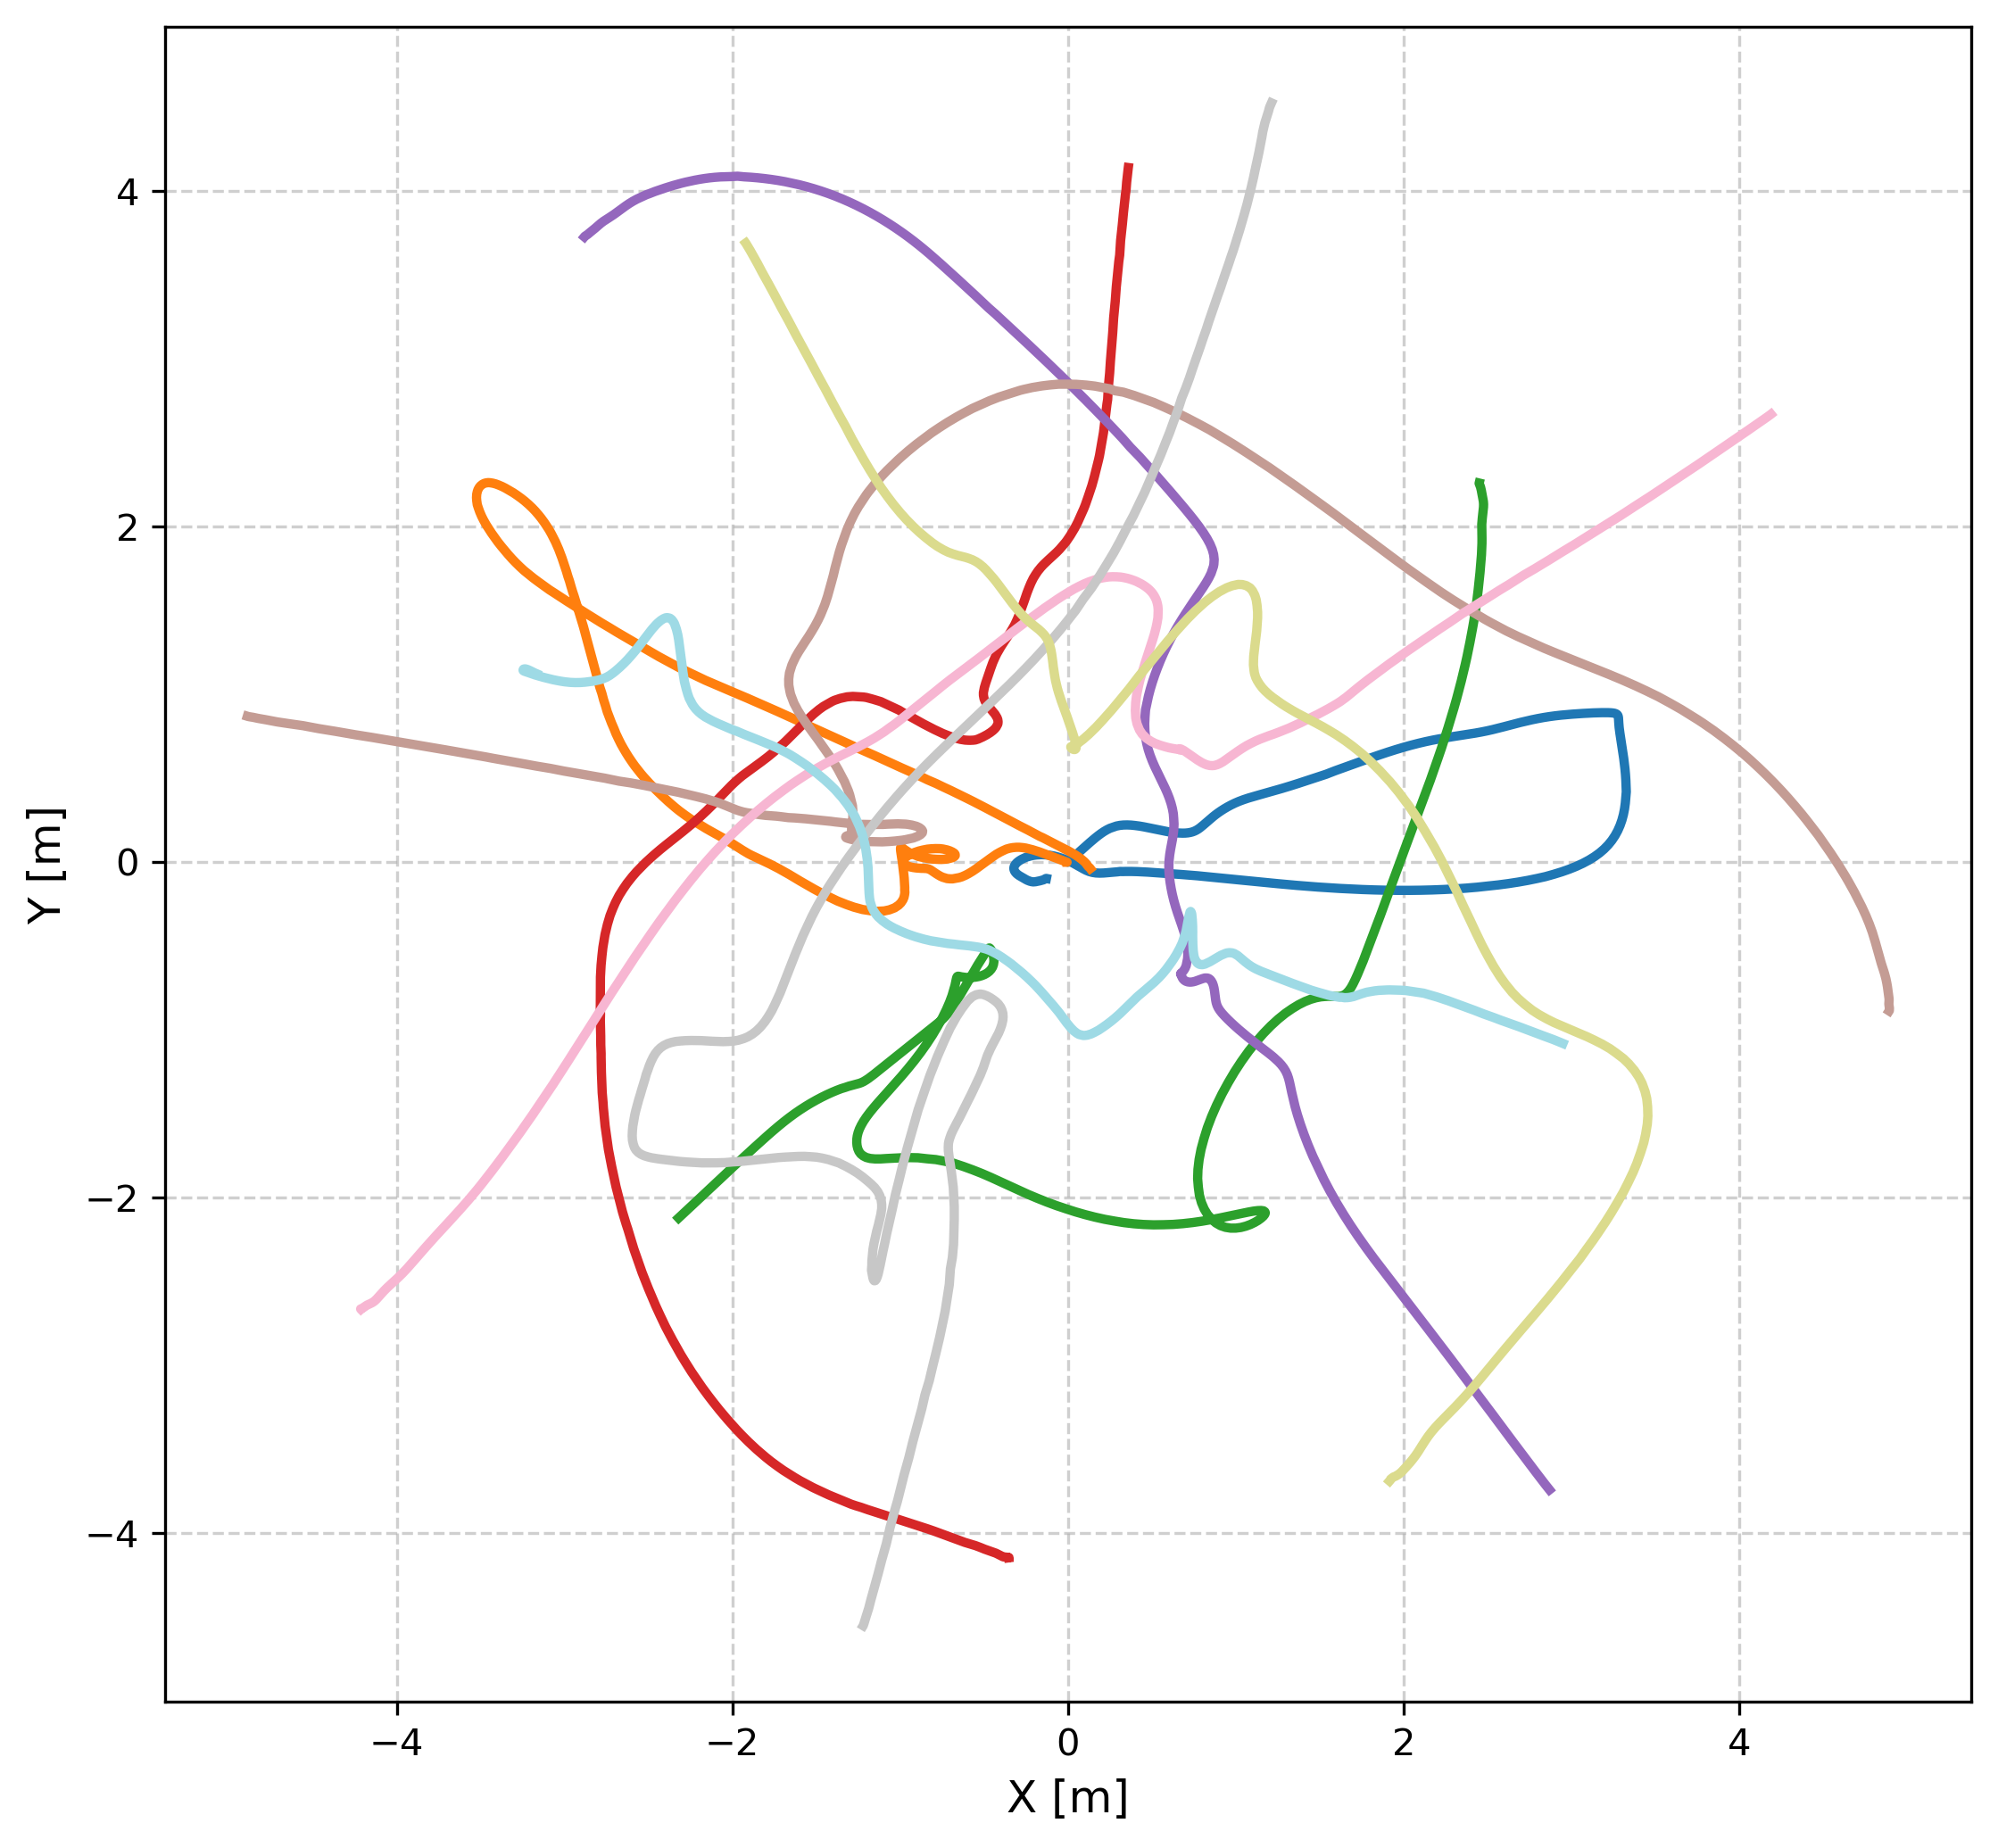
\includegraphics[width=0.48\textwidth, height=0.48\textwidth]{./fig/plots/sphere_3d_top_down.png}
        }
        \subfloat[Side View (X-Z)] {
        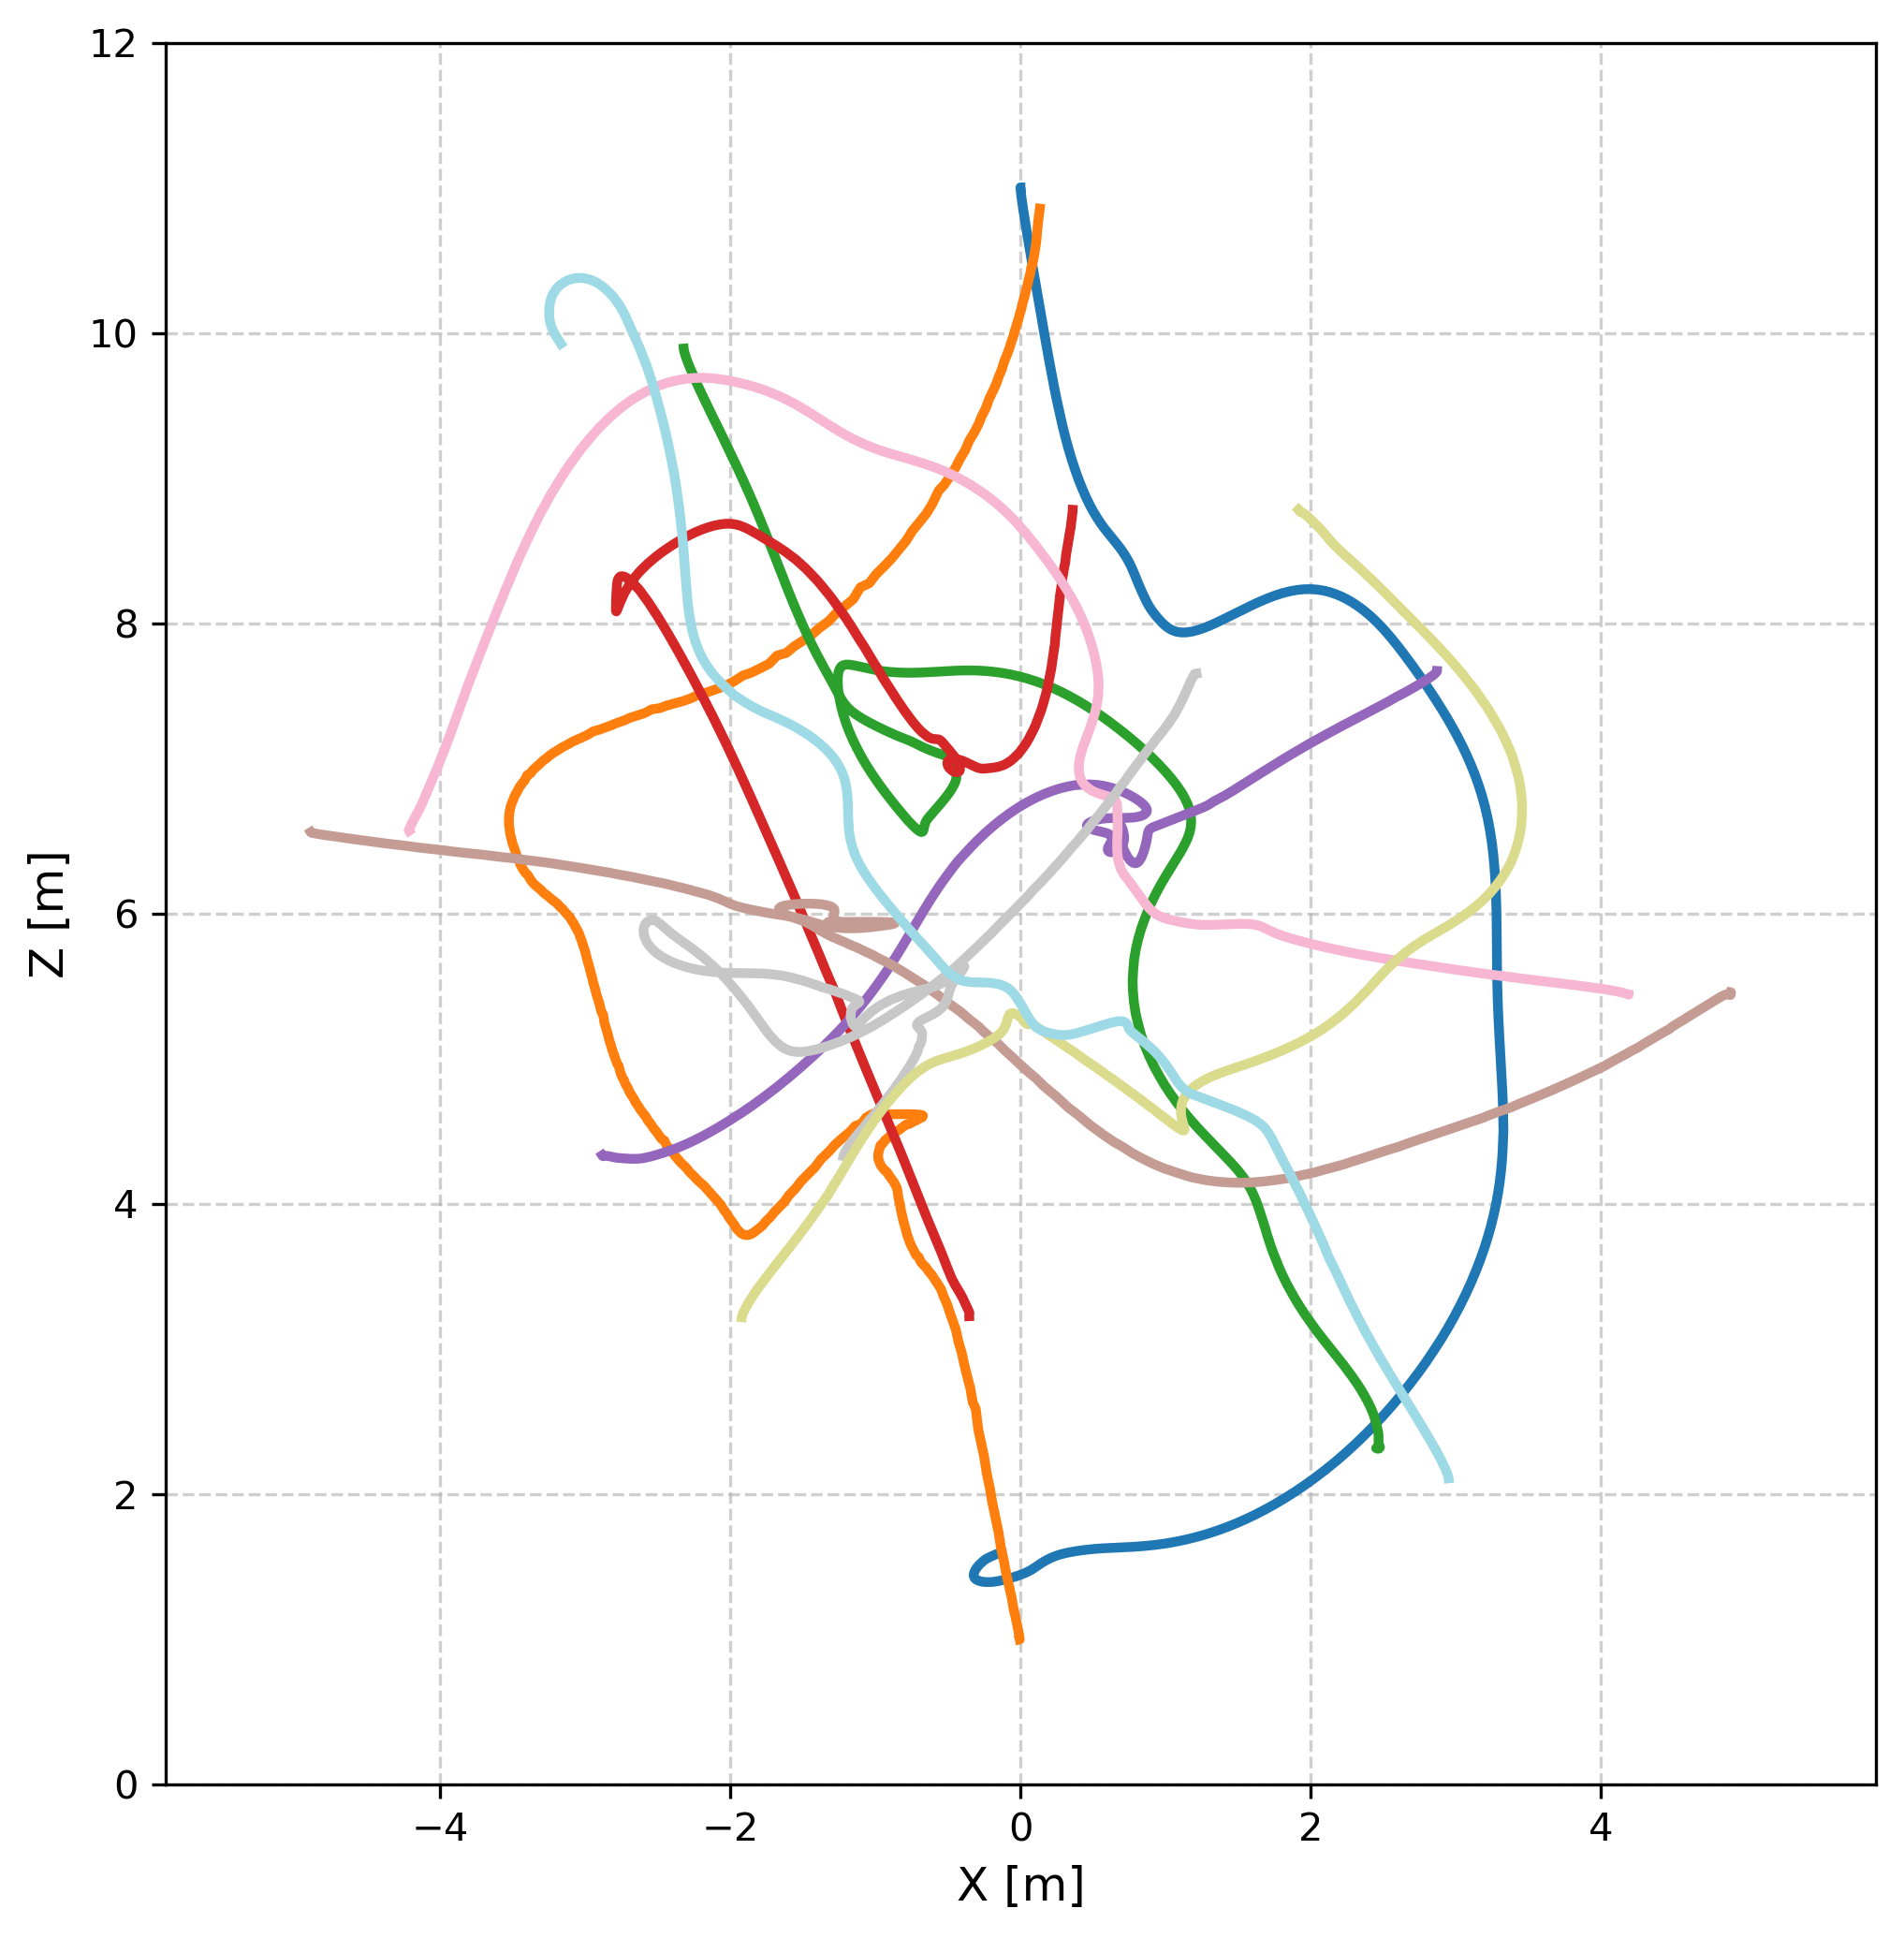
\includegraphics[width=0.48\textwidth, height=0.48\textwidth]{./fig/plots/sphere_3d_side.png}
        }
        \caption{
            Trajectories in a \ac{3D} spherical crossing.
        }
        \label{}
    \end{figure}
% \chapter{Appendix A}

\end{document}
